%
% FH Technikum Wien
% !TEX encoding = UTF-8 Unicode
%
% Erstellung von Master- und Bachelorarbeiten an der FH Technikum Wien mit Hilfe von LaTeX und der Klasse TWBOOK
%
% Um ein eigenes Dokument zu erstellen, müssen Sie folgendes ergänzen:
% 1) Mit \documentclass[..] einstellen: Master- oder Bachelorarbeit, Studiengang und Sprache
% 2) Mit \newcommand{\FHTWCitationType}.. Zitierstandard festlegen (wird in der Regel vom Studiengang vorgegeben - bitte erfragen)
% 3) Deckblatt, Kurzfassung, etc. ausfüllen
% 4) und die Arbeit schreiben (die verwendeten Literaturquellen in Literature.bib eintragen)
%
% Getestet mit TeXstudio mit Zeichenkodierung ISO-8859-1 (=ansinew/latin1) und MikTex unter Windows
% Zu beachten ist, dass die Kodierung der Datei mit der Kodierung des paketes inputenc zusammen passt!
% Die Kodierung der Datei twbook.cls MUSS ANSI betragen!
% Bei der Verwendung von UTF8 muss dnicht nur die Kodierung des Dokuments auf UTF8 gestellt sein, sondern auch die des BibTex-Files!
%
% Bugreports und Feedback bitte per E-Mail an latex@technikum-wien.at
%
% Versionen
% *) V0.7: 9.1.2015, RO: Modeline angepasst und verschoben
% *) V0.6: 10.10.2014, RO: Weitere Anpassung an die UK
% *) V0.5: 8.8.2014, WK: Literaturquellen überarbeitet und angepasst
% *) V0.4: 4.8.2014, WK: Initalversion in SVN eingespielt
%
\documentclass[MMR,Master,english]{twbook}
\usepackage[utf8]{inputenc}
\usepackage[T1]{fontenc}
%
% Hier biblatex & Biber konfigurieren; Vergessen Sie nicht, dass Sie biber verwenden müssen um eine Bibliothek zu erzeugen
%
\usepackage[backend=biber, style=numeric, sorting=none]{biblatex}
\addbibresource{Literature.bib}
%
% Bei Bedarf bitte hier die Syntax-Highlightings anpassen
%
% own 
\usepackage{hyperref}
\usepackage{float}
\usepackage{comment}
\usepackage{csquotes}
\usepackage{pgfplots}
\usepackage{soul}
\usepackage{color}
\usepackage{xcolor}  % Required for custom colors
\sethlcolor{blue}
\setcounter{secnumdepth}{3} % in text 
\setcounter{tocdepth}{3} % contents
\usepackage{longtable}
\usepackage{pdflscape}
\usepackage{rotating}
\usepackage{tikz}
\usepackage{setspace}
\usetikzlibrary{shapes,arrows}
\usetikzlibrary{positioning}

\hypersetup{
    colorlinks=true, % Aktiviert farbige Links
    linkcolor={rgb,255:red,0;green,0;blue,255}, % Interne Links (z.B. Sections)
    citecolor=orange, % Zitate
    urlcolor={rgb,255:red,128;green,0;blue,128} % URLs
}

%
% Platzierungsoptionen 
%
\usepackage[final]{listings}
\lstset{captionpos=b, numberbychapter=false,caption=\lstname,frame=single, numbers=left, stepnumber=1, numbersep=2pt, xleftmargin=15pt, framexleftmargin=15pt, numberstyle=\tiny, tabsize=3, columns=fixed, basicstyle={\fontfamily{pcr}\selectfont\footnotesize}, keywordstyle=\bfseries, commentstyle={\color[gray]{0.33}\itshape}, stringstyle=\color[gray]{0.25}, breaklines, breakatwhitespace, breakautoindent}
\lstloadlanguages{[ANSI]C, C++, python, [gnu]make, gnuplot, Matlab}

%Formatieren des Quellcodeverzeichnisses
\makeatletter
% Setzen der Bezeichnungen für das Quellcodeverzeichnis/Abkürzungsverzeichnis in Abhängigkeit von der eingestellten Sprache
\providecommand\listacroname{}
\@ifclasswith{twbook}{english}
{%
    \renewcommand\lstlistingname{Code}
    \renewcommand\lstlistlistingname{List of Code}
    \renewcommand\listacroname{List of Abbreviations}
}{%
    \renewcommand\lstlistingname{Quellcode}
    \renewcommand\lstlistlistingname{Quellcodeverzeichnis}
    \renewcommand\listacroname{Abkürzungsverzeichnis}
}
% Wenn die Option listof=entryprefix gewählt wurde, Definition des Entyprefixes für das Quellcodeverzeichnis. Definition des Macros listoflolentryname analog zu listoflofentryname und listoflotentryname der KOMA-Klasse
\@ifclasswith{scrbook}{listof=entryprefix}
{%
    \newcommand\listoflolentryname\lstlistingname
}{%
}
\makeatother
\newcommand{\listofcode}{\phantomsection\lstlistoflistings}

% Die nachfolgenden Pakete stellen sonst nicht benötigte Features zur Verfügung
\usepackage{blindtext}
%
% Einträge für Deckblatt, Kurzfassung, etc.
%
\title{Virtualisierung eines Echtzeit-Betriebssystems zur Steuerung eines Roboters mit Schwerpunkt auf die
Einhaltung der Echtzeit}
\author{Halil Pamuk, BSc}
\studentnumber{51842568}
%\author{Titel Vorname Name, Titel\and{}Titel Vorname Name, Titel}
%\studentnumber{XXXXXXXXXXXXXXX\and{}XXXXXXXXXXXXXXX}
\supervisor{Sebastian Rauh, MSc. BEng}
%\supervisor[Begutachter]{Titel Vorname Name, Titel}
%\supervisor[Begutachterin]{Titel Vorname Name, Titel}
%\secondsupervisor{Titel Vorname Name, Titel}
%\secondsupervisor[Begutachter]{Titel Vorname Name, Titel}
%\secondsupervisor[Begutachterinnen]{Titel Vorname Name, Titel}
\place{Wien}
\kurzfassung{Virtualisierung von Echtzeitbetriebssystemen für die Robotersteuerung bietet viele Vorteile im Vergleich zu herkömmlichen hardwarebasierten Ansätzen. Lösungen, die auf reiner Hardware basieren, sind oft für einen bestimmten Zweck gebaut und daher in ihrer Flexibilität eingeschränkt. Es ist schwierig, die Hardware-Topologie an neue Anforderungen anzupassen, und es kann kostspielig sein, insbesondere bei der Skalierung von Operationen. Der physische Zugang für Updates und Wartung ist herausfordernd, was zu Ausfallzeiten und Produktivitätsverlusten führt. Während die Virtualisierung diese Probleme adressiert, führt sie zu erhöhtem Overhead und Latenz.

\bigskip \noindent Diese Arbeit untersucht die Virtualisierung des proprietären Salamander 4-Betriebssystems unter Verwendung von QEMU/KVM. Salamander 4 wird mit Yocto gebaut und verwendet harte Echtzeit mit Xenomai 3. Das Hauptziel besteht darin, die Latenzlücke zwischen den virtualisierten und den Bare-Metal-Versionen zu überbrücken, um ein deterministisches und zuverlässiges Verhalten zu gewährleisten, das für Echtzeit-Roboteranwendungen entscheidend ist.
	
\bigskip \noindent Erste Latenzmessungen zeigten eine signifikante Leistungslücke zwischen dem Bare-Metal- und dem virtualisierten Setup. Daher wird ein umfangreicher Tuning-Prozess durchgeführt, um Echtzeit-Performance und Determinismus zu erreichen. Diese Modifikationen umfassen Konfigurationen, die das BIOS, den Kernel, das Host-Betriebssystem, die QEMU/KVM-Virtualisierungsschicht und das Salamander 4-Betriebssystem (Gast) selbst betreffen. Die Worst-Case-Latenz wurde von 707.622\textmu s auf 17.134\textmu s reduziert, was der Bare-Metal-Performance von 10.709\textmu s nahekommt. Darüber hinaus wird die Verbesserung der Echtzeit-Performance und des Determinismus anhand einer Roboteranwendung validiert, bei der die abgestimmte Virtualisierung mit der nicht abgestimmten und der Hardware-Version verglichen wird.
	
\bigskip \noindent Insgesamt bietet diese Arbeit eine umfassende Blaupause, um ein virtualisiertes Gastsystem in einem Host-System mit deterministischem Verhalten echtzeitfähig zu machen.}
\schlagworte{Virtualisierung, Echtzeitsysteme, Latenzreduktion, Robotiksteuerung}

\outline{Virtualization of real-time operating systems systems for robotic control has many advantages in comparison to traditional hardware-based approaches. Solutions based on pure hardware are often built for a distinct purpose and are hence limited in flexibility. It is difficult to adapt the hardware topology to new requirements and can be costly, especially when scaling operations. Physical access for updates and maintenance is challenging, leading to downtime and lost productivity. While virtualization addresses these issues, it introduces increased overhead and latency. 
	
\bigskip \noindent This thesis investigates the virtualization of the proprietory Salamander 4 operating system, using QEMU/KVM. Salamander 4 is built with Yocto and employs hard real-time with Xenomai 3. The primary objective is to bridge the latency gap between the virtualized and bare metal versions in order to ensure deterministic and reliable behavior, which is crucial for real-time robotic applications.

\bigskip \noindent Initial latency measurements revealed a significant performance gap between the bare metal and virtualized setup. Thus, an extensive tuning process is carried out to achieve real-time performance and determinism. These modifications involve configurations spanning the BIOS, kernel, host operating system, QEMU/KVM virtualization layer, and the Salamander 4 operating system (guest) itself. The worst-case latency was brought down from 707.622\textmu s to 17.134\textmu s, closely aligning with the bare metal performance of 10.709\textmu s. In addition, the improvement in real-time performance and determinism is validated using a robotic application, where the tuned virtualization is compared with the untuned and the hardware version.

\bigskip \noindent Alltogether, this thesis provides a comprehensive blueprint for making a virtualized guest system real-time capable in a host system with deterministic behavior.}
\keywords{Virtualization, Real-Time Systems, Latency Reduction, Robotic Control}

\acknowledgements{First, I would like to thank my supervisor, Sebastian Felix Rauh MSc. BEng., for his expert guidance and assistance throughout this master's thesis. His insightful answers to all my questions and his calming presence helped me stay focused and composed.

\bigskip \noindent I want to thank my wife, Nour Pamuk, for her unwavering support, love, and patience. She gave me the strength to overcome this challenge. This work is as much hers as it is mine.

\bigskip \noindent Lastly, I am deeply grateful to my parents, Semra Pamuk and Mehmet Pamuk, and to my close family for their understanding and encouragement during my studies. Without their unconditional love and support, this work would not have been possible.}

\begin{document}

\maketitle
%
% .. und hier beginnt die eigentliche Arbeit. Viel Erfolg beim Verfassen!
%
%Die folgende Gliederung von Bachelor- und Masterarbeiten ist für die Robotik-Studiengänge
%verpflichtend vorgeschrieben.
%
%- Deckblatt
%- Eidesstattliche Erklärung (digital signiert)
%- Kurzfassung und Abstract mit Schlüsselwörtern/Keywords
%- Danksagung (optional)
%- Inhaltsverzeichnis

%- Einleitung (die genannten Punkte müssen keine eigenen Unterkapitel sein, müssen aber aus der Einleitung klar hervorkommen):
%   - Stand der Technik
%   - Problem- und Aufgabenstellung
%   - Zielsetzung
%- Hauptteil -> Gliederung je nach Thema
%   - Methodik
%   - Resultate
%   - Wirtschaftliche Betrachtung (optional)
%   - Diskussion
%- Zusammenfassung und Ausblick

%- Literaturverzeichnis
%- Abbildungsverzeichnis
%- Tabellenverzeichnis
%- Abkürzungsverzeichnis (optional)
%- Glossar (optional)
%- Anhang (optional)

\chapter{Introduction}\label{cha:introduction}
In today's industrial production and automation, robot systems are well established and of crucial importance. Robots must react to their environment and perform time-critical tasks within strict time constraints. Delays or errors can have catastrophic consequences in some cases. Modern operating systems nowadays are categorized into two types:  general-purpose operating systems (GPOS) and real-time operating systems (RTOS). The key difference is whether the system is time-critical or not~\cite{canbazPerformanceAnalysisRealtime2022}. In a traditional GPOS, such as Windows or Linux-based distributions, a high-priority task cannot interrupt a kernel operation, as illustrated in Figure~\ref{fig:kernel_generic}. This makes them not suitable for real-time requirements, as they cannot guarantee deterministic execution times.

\begin{figure}[H]
	\centering
	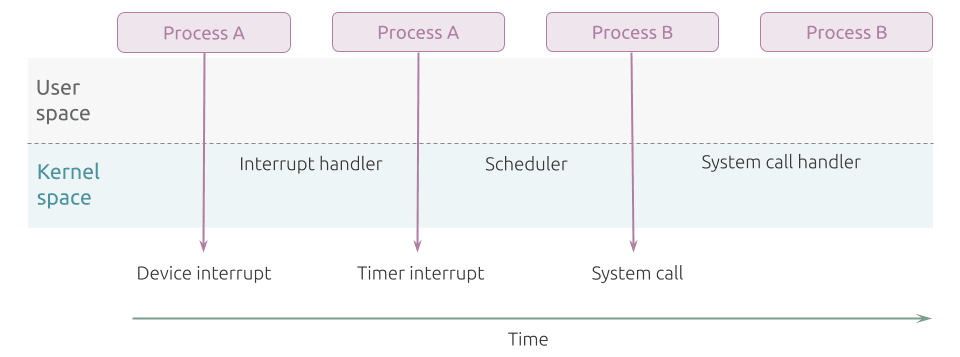
\includegraphics[width=0.75\columnwidth]{img/introduction/kernel_generic.png}
	\caption[Non-preemptible Kernel]{Non-preemptible Kernel~\cite{WhatRealtimeLinux}}
	\label{fig:kernel_generic}
\end{figure}

\noindent However, in an RTOS, a high-priority process can interrupt a lower-priority task, even if it is in the middle of a kernel operation, as shown in Figure~\ref{fig:kernel_rt} RTOS are specifically designed to react to events within fixed time limits and prioritise the execution of high-priority processes.

\begin{figure}[H]
	\centering
	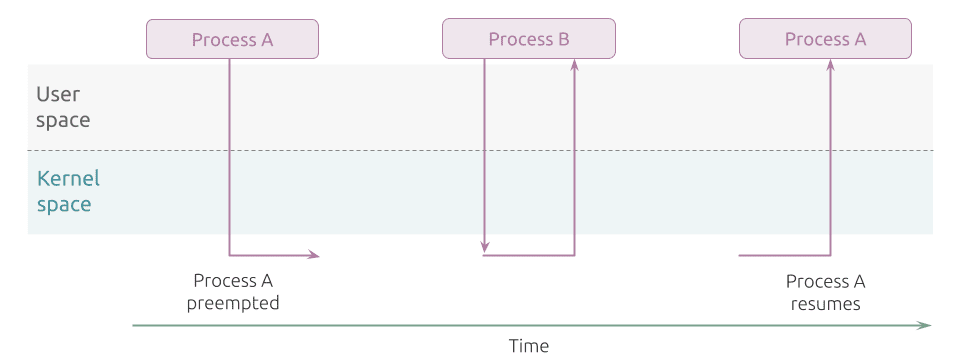
\includegraphics[width=0.75\columnwidth]{img/introduction/kernel_rt.png}
	\caption[Preemptible Kernel]{Preemptible Kernel~\cite{WhatRealtimeLinux}}
	\label{fig:kernel_rt}
\end{figure}

\noindent Many Linux distributions can function as both GPOS and RTOS with kernel modifications.

\section{Real-Time Operating Systems}
\noindent The RTOS structure is visualized in Figure~\ref{fig:rtos_structure}.The core component of an RTOS that enables real-time capabilities is the kernel. It is responsible for managing system resources, scheduling tasks, and ensuring deterministic behavior~\cite{malallahComprehensiveStudyKernel2021}. It employs preemptive scheduling mechanisms to allow high-priority tasks to preempt lower-priority tasks, ensuring that time-critical tasks are not delayed. Additionally, RTOS kernels are designed to allocate and manage memory resources efficiently and minimize interrupt latency, which is crucial for real-time applications that require immediate response to external events~\cite{wangRealtimeEmbeddedSystems2017}.

\begin{figure}[H]
	\centering
	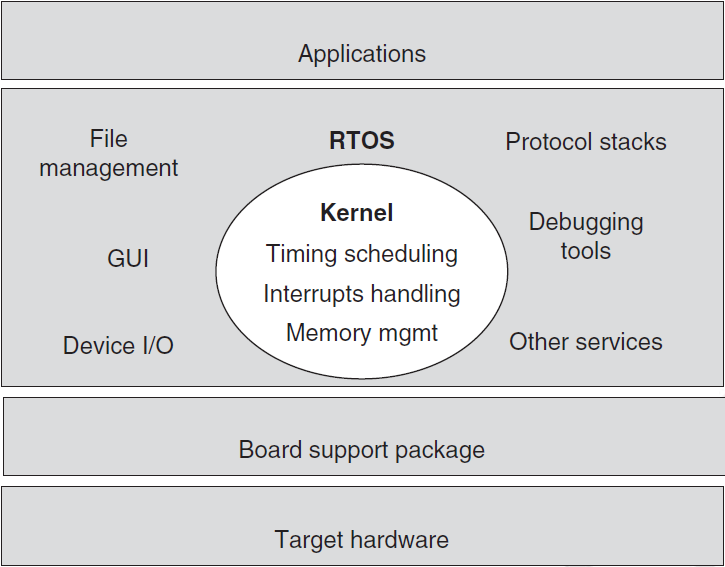
\includegraphics[width=0.50\columnwidth]{img/introduction/rtos_structure.png}
	\caption[RTOS Structure]{RTOS Structure~\cite{wangRealtimeEmbeddedSystems2017}}
	\label{fig:rtos_structure}
\end{figure}

\noindent In these real-time operating system, task scheduling is based on so-called priority-based preemptive scheduling~\cite{buttazzoHardRealtimeComputing2024}. Each task in a software application is assigned a priority. A higher priority means that a faster response is required. Preemptive task scheduling ensures a very fast response. Preemptive means that the scheduler can stop a currently running task at any point if it recognizes that another task needs to be executed immediately. The basic rule on which priority-based preemptive scheduling is based is that the task with the highest priority that is ready to run is always the task that must be executed. So if both a task with a lower priority and a task with a higher priority are ready to run, the scheduler ensures that the task with the higher priority runs first. The lower priority task is only executed once the higher priority task has been processed.

\bigskip \noindent Real-time systems are usually classified as either soft or hard real-time systems~\cite{lipariRealTimeSchedulingHard2015}. The difference lies exclusively in the consequences of a violation of the time limits~\cite{amarpreetHardRealTime2009}. Hard real-time is when the system stops operating if a deadline is missed, which can have catastrophic consequences. Soft real-time exists when a system continues to function even if it cannot perform the tasks within a specified time. If the system has missed the deadline, this has no critical consequences. The system continues to run, although it does so with undesirably lower output quality~\cite{queirozTestingLimitsGeneralpurpose2023}.

\section{Application Context}\label{sec:application_context}
This section briefly defines the context and scope within which this master's thesis was composed, highlighting the specific contributions and requirements set by SIGMATEK GmbH \& Co KG~\cite{pixelartSIGMATEKKompletteAutomatisierungssysteme}.

\begin{itemize}
	\item This work was written at SIGMATEK GmbH \& Co KG, a company that researches, develops, produces, and distributes automation technology for industrial machinery and plant engineering. SIGMATEK uses its own custom Linux-based operating system, to be run on their self-manufactured CPUs. This operating system will be referred to as ``Salamander 4'' in this work. The details of Salamander 4 are explained in Chapter~\ref{sec:guest_operating_system}.
	\item Salamander 4 was created with Yocto~\cite{WelcomeYoctoProject}, an open-source project that helps develop custom Linux-based systems. Yocto is discussed in Section~\ref{sec:yocto}.
	\item Salamander 4 is virtualized through Quick emulator (QEMU), an open-source emulator and virtualizer that allows to run different operating systems on a computer QEMU is described in Section~\ref{sec:qemu}.
	\item Salamander 4 employs hard real-time with Xenomai 3~\cite{XenomaiXenomai}, a real-time framework for Linux that enables deterministic and low-latency performance. Xenomai 3 is detailed in Section~\ref{sec:xenomai}.
	\item The goal is to virtualize Salamander 4 and approach the performance of bare metal (hardware) through real-time performance tunings, focussing on latency requirements set by SIGMATEK. These modifications are subject of Chapter~\ref{sec:real-time_tunings}.
	\item The \texttt{latency} tool of the Xenomai suite to measure the scheduling latency of the real-time OS was suggested to use by SIGMATEK. The goal was set to achieving latency values below 50 microseconds in the duration of the measuremenet.
	\item SIGMATEK uses the VARAN bus for communication between machines and systems, a real-time Ethernet network that was specially developed for industrial automation. Its operating principle is outlined in Section~\ref{sec:varan}.
	\item For the purpose of replacing the physical CPU, SIGMATEK provided a PCI Insert Card module PCV 522, that was plugged into the PC, as explained in Subsection~\ref{subsec:setup_experiment_virtualized}. This component could then be used to communicate with the Input/Output peripherals, just like the physical CPU could when the I/O modules were attached to it. Subsequently, the PCV 522 module of SIGMATEK was connected with the Pulse Width Module PW 022 of SIGMATEK over the VARAN bus and the VI 021 module of SIGMATEK serving as the power supply.
	\item The robotic application from Chapter~\ref{sec:robotic_application} was written in Lasal Class 2, an object oriented programming tool of SIGMATEK and part of SIGMATEK`s Engineering Platform LASAL, with client-server technology and graphic representation.
\end{itemize}
\section{Related Work and State of the Art}
This master’s thesis builds upon a number of previous studies in the field of virtualization of real-time systems and the inherent latency. In this section, the most influential studies are presented and their relevance to the work is addressed.

\bigskip \noindent \citeauthor{perneelRealtimeCapabilitiesStandard2015}~\cite{perneelRealtimeCapabilitiesStandard2015} mention in their work that Linux was initially developed as a general purpose operating system without real-time applications in mind. They talk about the evolution of real-time behavior in the standard Linux kernel and state that it has recently gained popularity among the real-time community, largely due to its open-source nature and stability. The authors explain how to transform Linux into a real-time operating system by implementing the PREEMPT-RT patches. The paper also emphasizes some kernel configurations that ensure that the system's real-time behavior is preserved during runtime. Even though these modifications to the kernel enable soft real-time performance, the authors underline the fundamental rule in real-time software, that latency improvements have a negative impact on throughput and kernel performance. This is due to the added overhead of the \texttt{CONFIG\_PREEMPT\_RT} option. They concluded with their Linux build and a testing application that Linux can be a viable option for real-time applications, if it is correctly configured. \citeauthor{reghenzaniRealTimeLinuxKernel2020}~\cite{reghenzaniRealTimeLinuxKernel2020} provide an extensive overview on the real-time Linux kernel research, specifically on the PREEMPT RT patch. \citeauthor{adamRealTimePerformanceResponse2021}~\cite{adamRealTimePerformanceResponse2021} applied the PREEMPT\_RT patch on both Raspberry Pi 3 and BeagleBone Black and achieved significantly lower latencies compared to standard Linux kernels.

\bigskip \noindent \citeauthor{cinqueVirtualizingMixedCriticalitySystems2022}~\cite{cinqueVirtualizingMixedCriticalitySystems2022} survey different virtualization approaches, including separation kernels, microkernels, enhanced general-purpose hypervisors, and lightweight virtualization solutions like containers and unikernels. Similarly, \citeauthor{sandstromVirtualizationTechnologiesEmbedded2013}~\cite{sandstromVirtualizationTechnologiesEmbedded2013}, and~\citeauthor{taccariEmbeddedRealTimeVirtualization2014}~\cite{taccariEmbeddedRealTimeVirtualization2014} discuss and compare the current state-of-the-art in virtualization technologies with a focus on embedded real-time platforms. The latter emphasizes, that research on real-time systems is focusing on virtualization and multicore scheduling and underlines that flexibility and cost are key metrics. Both works acknowledge the great benefits of virtualization, that is, reducing overall hardware costs, since all non-critical activities and real-time control tasks can run on the same hardware. In addition,~\citeauthor{javierperezHowRealTime2022}~\cite{javierperezHowRealTime2022} state that hardware-based Programmable Logic Controllers (PLCs) are costly to maintain and lack the flexibility needed for modern, resource-intensive applications like Machine Learning (ML) or Artificial Intelligence (AI).

\bigskip \noindent Despite the promising advantages of virtualization, one must be aware of the potential drawbacks of it, too.~\citeauthor{guStateoftheArtSurveyRealTime2012}~\cite{guStateoftheArtSurveyRealTime2012} highlight issues like lock-holder preemption and task-grain scheduling.~\citeauthor{garcia-vallsChallengesRealtimeVirtualization2014}~\cite{garcia-vallsChallengesRealtimeVirtualization2014} identify challenges in supporting real-time applications in the cloud, including resource management, quality of service guarantees, temporal and spatial isolation, and network performance.~\citeauthor{scordinoRealTimeVirtualizationIndustrial2020}~\cite{scordinoRealTimeVirtualizationIndustrial2020} address the challenge of interference on shared hardware resources, which can degrade real-time performance.

\bigskip \noindent \citeauthor{maPerformanceTuningKVMbased2013}~\cite{maPerformanceTuningKVMbased2013}~\cite{junzhangPerformanceAnalysisKVMBased2010} describe in their work how KVM impacts the real-time performance, which has helped this work gain insight into the base overhead of virtualization. When a physical interrupt occurs while the guest RTOS is running, there are at least six stages that need to be traversed before the interrupt can be delivered to the guest RTOS. Once the interrupt is delivered to the guest RTOS, it incurs additional latency, called Interrupt Routine Time (IRT), since there is also the time between when an interrupt is recognized and the first instruction of the corresponding interrupt service routine (ISR) of the guest OS is started. These stages are the primary sources of latencies caused by KVM, they are briefly described in Figure~\ref{fig:kvm_stages}.
\vspace{2em}
\begin{figure}[H]
	\centering
	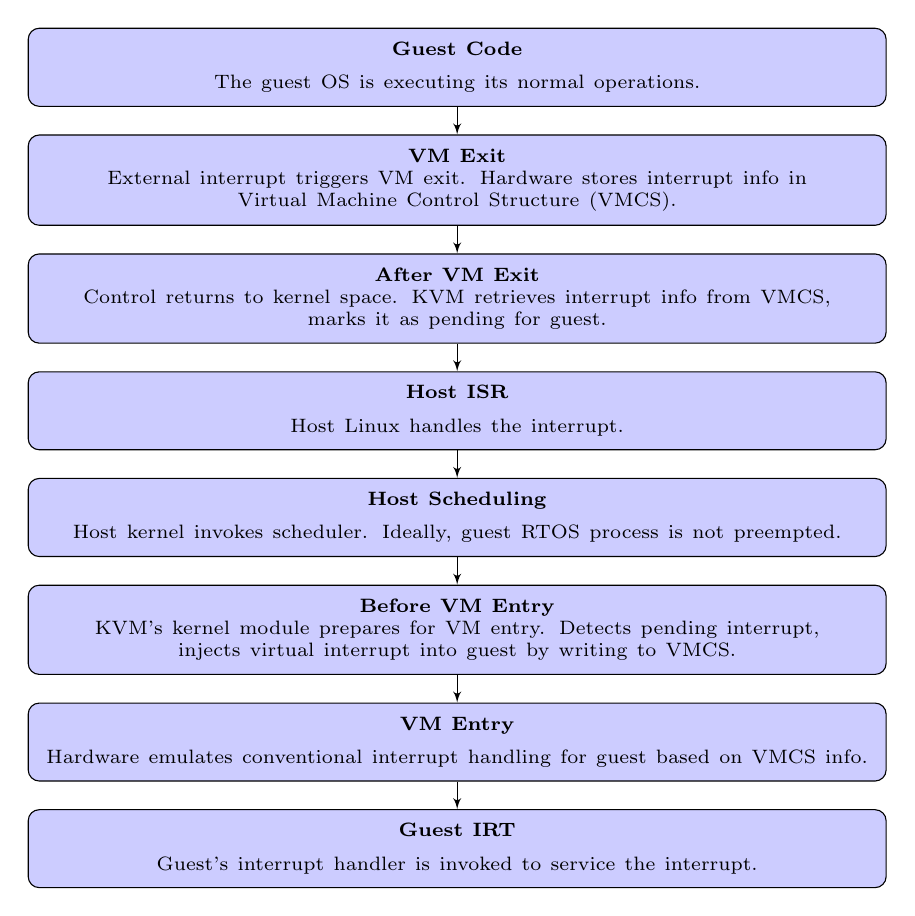
\begin{tikzpicture}[node distance = 0.35cm, auto, % Adjusted node distance
			block/.style={
					rectangle,
					draw,
					fill=blue!20,
					text width=30em,
					rounded corners,
					align=center,
					inner sep=0.5em
				},
			line/.style={draw, -latex'}
		]
		% Place nodes
		\node [block] (init) {\scriptsize \textbf{Guest Code}\\  The guest OS is executing its normal operations.};
		\node [block, below=of init] (vmexit) {\scriptsize \textbf{VM Exit}\\  External interrupt triggers VM exit. Hardware stores interrupt info in \\\vspace{-0.5em} Virtual Machine Control Structure (VMCS).};
		\node [block, below=of vmexit] (aftervmexit) {\scriptsize \textbf{After VM Exit}\\  Control returns to kernel space. KVM retrieves interrupt info from VMCS,\\\vspace{-0.5em} marks it as pending for guest.};
		\node [block, below=of aftervmexit] (hostisr) {\scriptsize \textbf{Host ISR}\\  Host Linux handles the interrupt.};
		\node [block, below=of hostisr] (hostscheduling) {\scriptsize \textbf{Host Scheduling}\\  Host kernel invokes scheduler. Ideally, guest RTOS process is not preempted.};
		\node [block, below=of hostscheduling] (beforevmentry) {\scriptsize \textbf{Before VM Entry}\\  KVM's kernel module prepares for VM entry. Detects pending interrupt,\\\vspace{-0.5em} injects virtual interrupt into guest by writing to VMCS.};
		\node [block, below=of beforevmentry] (vmentry) {\scriptsize \textbf{VM Entry}\\  Hardware emulates conventional interrupt handling for guest based on VMCS info.};
		\node [block, below=of vmentry] (guestirt) {\scriptsize \textbf{Guest IRT}\\  Guest's interrupt handler is invoked to service the interrupt.};
		% Draw edges
		\path [line] (init) -- (vmexit);
		\path [line] (vmexit) -- (aftervmexit);
		\path [line] (aftervmexit) -- (hostisr);
		\path [line] (hostisr) -- (hostscheduling);
		\path [line] (hostscheduling) -- (beforevmentry);
		\path [line] (beforevmentry) -- (vmentry);
		\path [line] (vmentry) -- (guestirt);
	\end{tikzpicture}
	\caption[Flowchart of Operations in a virtualized Environment]{Flowchart of Operations in a virtualized Environment (Own Figure, inspired by~\citeauthor{maPerformanceTuningKVMbased2013})}
	\label{fig:kvm_stages}
\end{figure}
\vspace{1em}

\noindent The paper also details several performance tuning methods, including CPU shielding and prioritization, which have been applied in this work.

\clearpage

\bigskip \noindent \citeauthor{broskyShieldedProcessorsGuaranteeing2003}~\cite{broskyShieldedProcessorsGuaranteeing2003} report in their work about the shielded CPU model for enhancing real-time performance in symmetric multiprocessor systems. By dedicating one or more CPUs to high-priority processes and interrupts, the goal is to provide deterministic execution of real-time applications and interrupt responses. The authors mention that there is no user interface for setting process CPU affinity in the standard Linux, while there is one for setting interrupt CPU affinity via the \texttt{/proc/irq/*/smp\_affinity} files. These files were used in this masther's thesis. According to the authors, the shielded CPU model is especially useful for tasks that require guaranteed interrupt response times, very fast interrupt responses and high-frequency, deterministic execution.

\bigskip \noindent In the course of writing this thesis, the white paper "Real-Time Performance Tuning Best Practice Guidelines for KVM-Based Virtual Machines"~\cite{RealTimePerformanceTuning2022} by Intel has been instrumental. Given that the working computer used for this work is equipped with an Intel processor, the guidelines presented in this document were particularly relevant and valuable for optimizing real-time performance in KVM-based virtual machines. Chapter~\ref{sec:real-time_tunings} contains an extensive tuning process, which involves configurations spanning the BIOS, kernel, host OS, QEMU/KVM virtualization layer, and the Salamander 4 OS itself. The document concludes that the described tuning methods effectively improve real-time performance for KVM-based VMs, even under heavy workloads.

\bigskip \noindent \citeauthor{yoonRealTimePerformanceAnalysis2009}~\cite{yoonRealTimePerformanceAnalysis2009} use some of these real-time tunings in their research, including CPU shielding, memory locking, and spinning nanosleep, for controlling humanoid robots equipped with around 60 servo motors and sensors. They implement EtherCAT for real-time communication of distributed devices whereas this thesis uses Varan. The authors highlight the importance of timely data processing in robots that collect data from their environment and respond accordingly through their sensors and actuators. The authors conclude with an experiment that their robotic system could achieve deterministic control of actuators and sensors even under heavy system load through the use of Linux with the real-time preemption patch. Their research has similarities to this master's thesis in terms of real-time tunings for robot control. However, this thesis includes also the virtualization aspect that is central.

\bigskip \noindent \citeauthor{kiszkaLinuxRealTimeHypervisor2009}~\cite{kiszkaLinuxRealTimeHypervisor2009} specifically focuses on Linux as a hypervisor and analyzes its real-time capabilities when using KVM and QEMU. Most importantly for this master's thesis, the author warns of starvation when the priorities of QEMU’s threads are raised and lifted into a real-time scheduling class. Starvation is when a process does not get the resources it needs for a long time because the resources are being allocated to other processes. A way to reduce this risk is by not using more virtual CPUs (vCPUs) than there are actual processor cores. Moreover, Linux has a feature that can limit how much CPU time all real-time tasks can use in the host system, which was an important information for the real-time tunings of this thesis later.

\clearpage

\bigskip \noindent \citeauthor{mckenneyRealTimeVs2008}~\cite{mckenneyRealTimeVs2008} addresses the overheads associated with real-time Linux when using KVM and QEMU. The author lists several sources of overhead, including memory locking to avoid page-fault latencies, increased overhead of locking and interrupts due to more-aggressive preemption, threaded interrupts that permit long-running interrupt handlers to be preempted by high-priority real-time processes, real-time task scheduling that requires global scheduling, high-resolution timers for tens-of-microseconds accuracy and precision, and preemptible RCU which has slightly higher read-side overhead than Classic RCU. These information helped understand the trade-offs involved in real-time Linux systems.

\bigskip \noindent \citeauthor{deoliveiraDemystifyingRealTimeLinux2020}~\cite{deoliveiraDemystifyingRealTimeLinux2020} critique the traditional \texttt{cyclictest} tool used for measuring scheduling latency, highlighting its limitations due to its black-box approach and lack of theoretical grounding. This is the main reason why this tool was not used to measure the scheduling latency in this work. Instead, the \texttt{latency} tool was used, as was determined in Chapter~\ref{sec:application_context}.

\section{Problem and Task Definition}
As stated previously, virtualization of real-time systems has many advantages in comparison to traditional hardware-based approaches. Solutions based on pure hardware are often built for a distinct purpose and are hence limited in flexibility. It is difficult to adapt the hardware topology to new requirements or new applications. Moreover, during periods when the demand is lower, expensive hardware may sit idle, leading to inefficient use of resources and a poor return on investment~\cite{gabrielResourceAwareParameterTuning2019}. Another crucial factor is of course the high cost factor associated with procuring and maintaining separate hardware for each real-time system~\cite{bhardwajVirtualizationCloudComputing2021}. Especially when organizations scale their operations, they have to add more physical machines, and the expenses rise rapidly~\cite{abbasiExploringOpenStackScalable2023}. Besides, one needs physical access to the hardware for any updates or maintenance, which is hard to achieve, especially for systems in remote or difficult-to-access locations. This can lead to system downtime and may not only disrupt the operations but can also result in lost productivity and potential revenue~\cite{mahfoudRealTimePredictiveMaintenanceBased2024}.

\bigskip \noindent Virtualization promises to overcome these challenges~\cite{queirozContainerbasedVirtualizationRealtime2024}~\cite{bhardwajVirtualizationCloudComputing2021}~\cite{cinqueEvaluatingVirtualizationFog2023}. However, virtualization also has its own challenges and pitfalls. The additional layers of abstraction can lead to increased overhead and latency~\cite{casiniLatencyAnalysisVirtualization2021}~\cite{zhangEvaluatingOptimizingVirtualization2010}. This is not desired and can be particularly problematic for real-time systems that require strict timing constraints. Making sure that tasks run predictably and on time in a virtualized environment, can be challenging. The hypervisor and other virtual components can cause variations in how long tasks take to execute~\cite{garcia-vallsChallengesRealtimeVirtualization2014}. When there are multiple virtual machines (VM) sharing the same physical resources, the VMs can affect each other's performance and consequently violate real-time constraints~\cite{queirozContainerbasedVirtualizationRealtime2024}.

\clearpage

\bigskip \noindent In this master's thesis, the task is the virtualization of a real-time operating system to control a robot, with a focus on compliance with real-time determinism. Chapter~\ref{cha:methodology} explains in detail the procedure, how this was tackled.  As already established in Section~\ref{sec:application_context}, Salamander 4 is built with Yocto, employs hard real-time with Xenomai 3 and is virtualized through QEMU/KVM. The initial latency values are measured with the \texttt{latency} program of the Xenomai tool suite. The initial situation is described in Section~\ref{sec:starting_situation}. In a nutshell, there is a significant initial gap in latency statistics between the virtualized Salamander 4 and the Salamander 4 on bare metal. For this reason, an extensive tuning process is carried out to achieve real-time performance and determinism. These modifications involve configurations spanning the BIOS, kernel, host OS, QEMU/KVM virtualization layer, and the Salamander 4 OS (guest) itself. The individual configurations are discussed in detail in Chapter~\ref{sec:real-time_tunings} and the modifications are justified with a clear explanation.

\section{Objective}
The goal is to bring the latency of the virtualized Salamander 4 closer to that of the hardware, thereby providing a comprehensive blueprint for making a virtualized guest system in a host system real-time capable with deterministic behavior. Section~\ref{sec:starting_situation} outlines the initial situation of this master's thesis and serves as the foundation for the real-time performance tunings discussed in Section~\ref{sec:real-time_tunings}. The objective is to achieve latency values below 50 microseconds during the measurement period through real-time tunings, with no outliers whatsoever. To determine and validate the performance of the tunings, the \texttt{latency} tool is used, as stated in Section~\ref{sec:application_context}. On top of that, the aim is to use a robotic application in a practical scenario to demonstrate and validate that the tunings significantly reduce latency and improve determinism compared to the unmodified virtualization.

\clearpage

\chapter{Methodology}\label{cha:methodology}

This chapter describes in detail all the theoretical concepts and boundary conditions as well as practical methods that contributed to achieving the objectives of this master's thesis.

\section{Host Operating System}\label{sec:host_operating_system}
The host operating system is the basis for the virtualization of the guest operating system. In the course of this work, it is continuously tuned to achieve real-time behavior and determinism. Table~\ref{tab:testbed_configuration} illustrates the specifications of the host.

\begin{table}[H]
	\centering
	\caption[Host Operating System Configuration]{Host Operating System Configuration}
	\label{tab:testbed_configuration}
	\setlength{\tabcolsep}{0.5em} % for the horizontal padding
	{\renewcommand{\arraystretch}{1.2}% for the vertical padding
		\begin{tabular}{|l|l|}
			\hline
			\textbf{CPU}            & Intel(R) Core(TM) i7-8700 CPU @ 3.20GHz, 6 cores \\ \hline
			\textbf{Memory}         & 4 $\times$ 8GB DDR4-2666/2400 MHz, 32GB          \\ \hline
			\textbf{GPU}            & Intel UHD Graphics 630 GPU                       \\ \hline
			\textbf{Storage}        & 500GB NVMe SSD                                   \\ \hline
			\textbf{BIOS}           & Dell Version 1.29.0                              \\ \hline
			\textbf{OS}             & Ubuntu 22.04.4 LTS                               \\ \hline
			\textbf{Kernel Version} & 6.8.0-40-generic                                 \\ \hline
		\end{tabular}}
\end{table}

\noindent Figure~\ref{fig:lstopo} is the output of the~\texttt{lstopo} command and visualizes the hardware nodes of the system, including CPU cores, caches, memory, and I/O devices.
\begin{figure}[H]
	\centering
	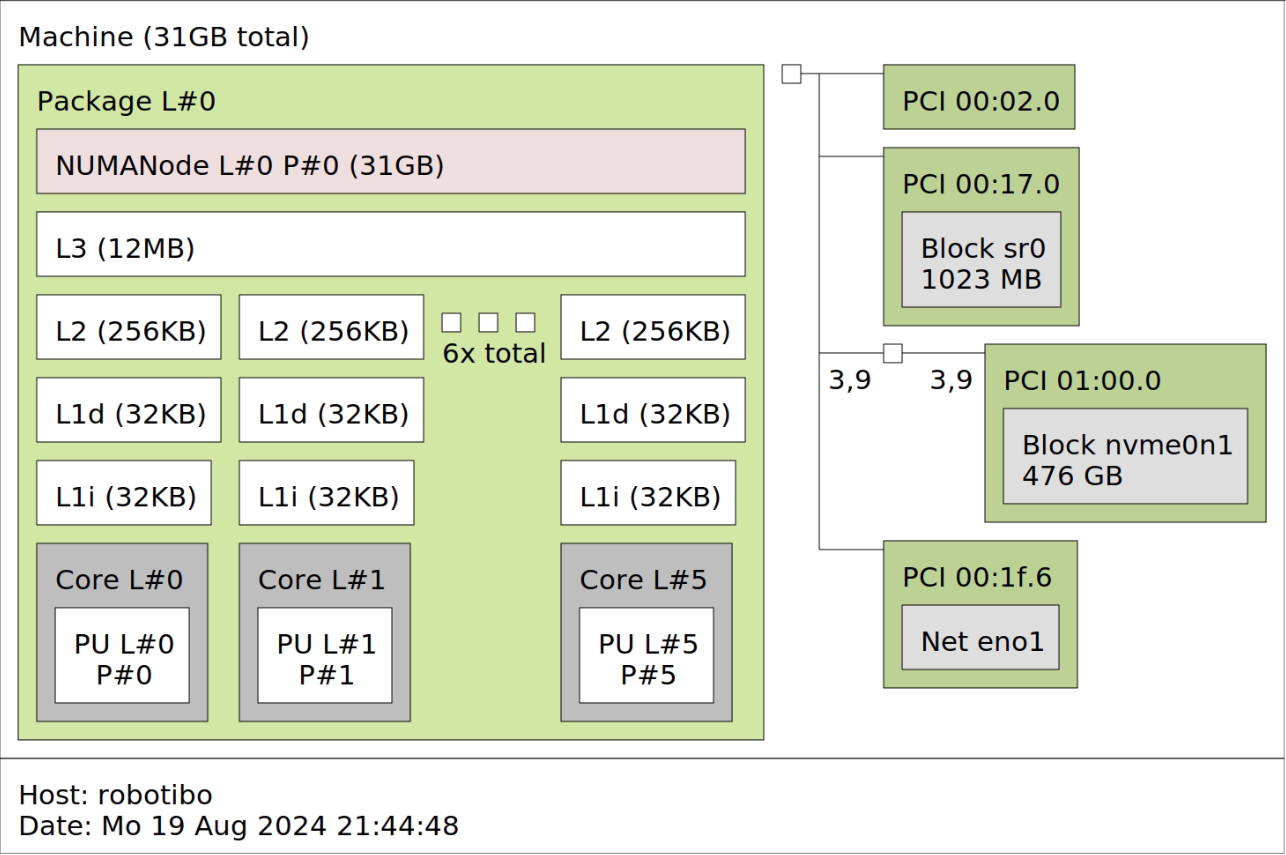
\includegraphics[width=0.55\columnwidth]{img/lstopo.png}
	\caption[Host Operating System Hardware Topology]{Host Operating System Hardware Topology}
	\label{fig:lstopo}
\end{figure}

\section{Guest Operating System}\label{sec:guest_operating_system}
This section briefly describes the guest operating system, Salamander 4.

\subsection{Structure}
\noindent Salamander 4 is the proprietary operating system of SIGMATEK. It is based on Linux version 5.15.94 and integrates Xenomai 3.2, a real-time development environment~\cite{XenomaiXenomai}. Salamander 4 is a 64-bit system, which refers to the x86\_64 architecture. The real-time behaviour is achieved through the use of Symmetric Multi-Processing (SMP) and Preemptive Scheduling (PREEMPT). In addition, it uses IRQPIPE to process interrupts in a way that meets the real-time requirements of the system. The output of the command~\texttt{uname -a} can be observed in code~\ref{output:uname_a_virt}.

\vspace{2em}
\begin{lstlisting}[name={System Information},label={output:uname_a_virt}]
root@sigmatek-core2:~# uname -a
Linux sigmatek-core2 5.15.94 #1 SMP PREEMPT IRQPIPE Tue Feb 14 18:18:05 UTC 2023 x86_64 GNU/Linux
\end{lstlisting}

\noindent Salamander 4 is powered by SIGMATEK's CP 841~\cite{CPUUnitsSIGMATEK} and is comprised of the following software modules:

\begin{itemize}
	\item \textbf{Operating system}: The operating system in a LASAL CPU manages the hardware and software resources of the system. It is provided in a completely PC-compatible manner, working with a standard PC BIOS.
	\item \textbf{Loader}: The loader is a part of the operating system that is responsible for loading programs from executables into memory, preparing them for execution and then running them.
	\item \textbf{Hardware classes}: Hardware classes in LASAL represent the different types of hardware components that can be controlled by the LASAL CPU. They help organize and manage the hardware components in a modular manner. The graphical hardware editor in LASAL allows for a true-to-detail simulation of the actual hardware.
	\item \textbf{Applications}: Applications are developed using LASAL CLASS 2~\cite{EngineeringToolLASAL}, a solution for automation tasks that supports object-oriented programming and design in compliance with IEC 61131-3.
\end{itemize}

\clearpage

\noindent These modules and the interfaces (indicated by an arrow) between them are shown in Figure~\ref{fig:lasal_cpu}.

\begin{figure}[H]
	\centering
	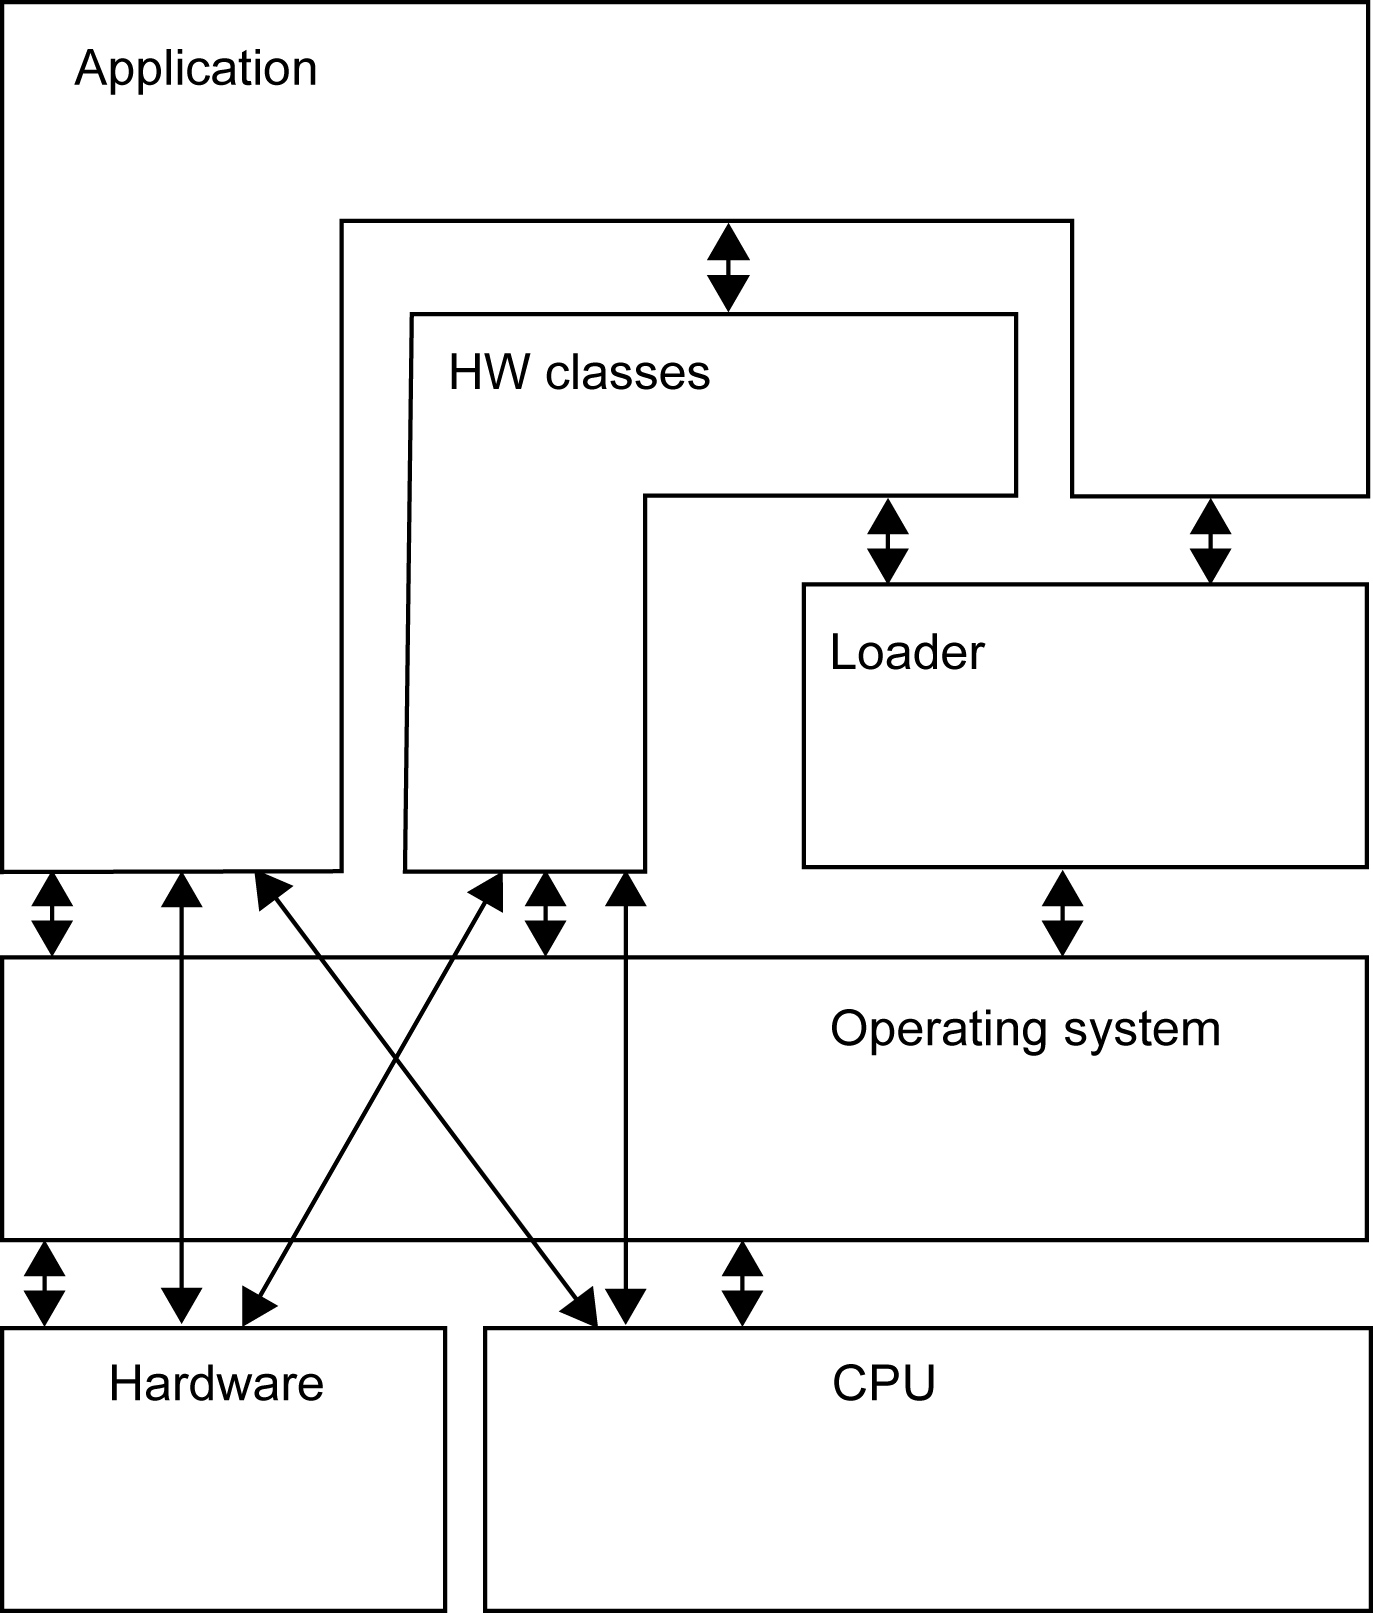
\includegraphics[width=0.5\columnwidth]{img/Software-Struktur_einer_LASAL_CPU.png}
	\caption[Structure of Salamander 4 CPU]{Structure of Salamander 4 CPU~\cite{LASALOSSIGMATEK}}
	\label{fig:lasal_cpu}
\end{figure}

\subsection{Memory Management}
\noindent For the sake of completeness, Figure~\ref{fig:memory_management} displays the memory management of Salamander 4. LRT stands for Lasal Runtime and creates an execution environment where applications developed using LASAL Class 2 can run- It provides real-time functions, data types, and other constructs for real-time programming.

\begin{figure}[H]
	\centering
	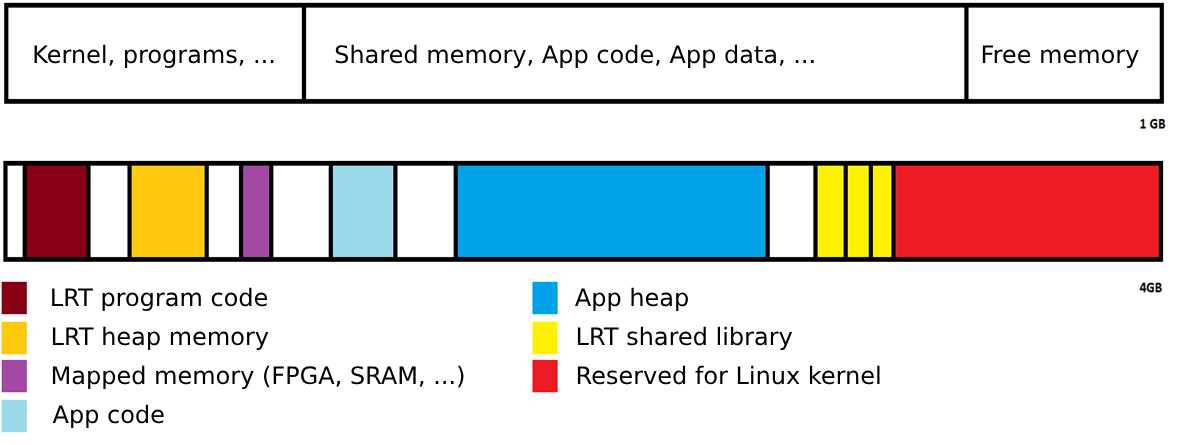
\includegraphics[width=0.8\columnwidth]{img/RAM_Memory_management.png}
	\caption[Memory Management of Salamander 4]{Memory Management of Salamander 4~\cite{LASALOSSIGMATEK}}
	\label{fig:memory_management}
\end{figure}

\clearpage

\section{QEMU}\label{sec:qemu}

QEMU~\cite{QEMU}. is an open-source emulator and virtualizer that allows to run operating systems and programs for one machine on a different machine. It can emulate different hardware architectures and is used in this thesis to emulate Salamander 4. When QEMU is used together with Kernel-based Virtual Machine (KVM), it can provide near-native performance by running code directly on the host CPU. The QEMU script used to emulate Salamander 4 and the meaning of the options are described in detail in Subsection \ref{subsec:salamander4-virtualization}.

\section{Yocto}\label{sec:yocto}

Salamander 4 is built with Yocto~\cite{WelcomeYoctoProject}, an open-source project that helps develop custom Linux-based operating systems for embedded devices. It is not a Linux version itself but a framework to make custom versions. From the kernel settings to the software packages included, almost everything in the Linux distribution can be adjusted with Yocto, hence it fits custom needs. Yocto organizes different components of the system into layers, making code management and updates easier. It builds the operating system with BitBake and automates the compilation and assembly of software. Upon generating the necessary files, Yocto provides a QEMU folder with the following components shown in Code~\ref{lst:ls}.

\vspace{2em}
\begin{lstlisting}[name={Contents of QEMU Folder for Salamander 4},label={lst:ls}]
    sigma_ibo@localhost:~/Desktop/salamander-image$ ls -1
    bzImage
    drive-c
    ovmf.code.qcow2
    qemu_def.sh
    salamander-image-sigmatek-core2.ext4
    stek-drive-c-image-sigmatek-core2.tar.gz
    vmlinux
    \end{lstlisting}

\noindent The following is a description of the components used for the virtualization of Salamander 4.

\begin{itemize}
	\item \textbf{bzImage}: Compressed Linux kernel image that is loaded by QEMU at system start. The short form ``bz`` stands for big-zipped.
	\item \textbf{drive-c}: Directory serving as C drive for QEMU, created and filled by qemu\_def.sh script.
	\item \textbf{ovmf.code.qcow2}: Firmware file for QEMU that enables UEFI boot process. ~\texttt{OVMF} stands for Open Virtual Machine Firmware,~\texttt{qcow2} is a format for disk image files used by QEMU, it stands for ``QEMU Copy On Write version 2''.
	\item \textbf{qemu\_def.sh}: Shell script that starts QEMU with required parameters to boot Salamamder 4 OS. It is described later in more detail.
	\item \textbf{salamander-image-sigmatek-core2.ext4}: Disk image of the Salamander 4 OS for the Sigmatek Core 2 platform. It uses the~\texttt{ext4} file system and serves as the root file system in the QEMU virtual machine, acting as the virtual hard drive.
	\item \textbf{stek-drive-c-image-sigmatek-core2.tar.gz}: Compressed tarball containing a pre-configured environment for the Salamander 4 OS. It is unpacked and sets up the~\texttt{drive-c/} directory with system and log files in the~\texttt{qemu\_def.sh} script.
	\item \textbf{vmlinux}: Uncompressed Linux kernel image, typically used for debugging.
\end{itemize}

\noindent The inital QEMU script after the custom Yocto build and the starting point for this work is shown in Code~\ref{script:qemu_def}. This script is used to start QEMU with required parameters to boot Salamamder 4 OS. It will be adjusted in Chapter~\ref{sec:real-time_tunings} in order to accompany real-time performance tunings.

\vspace{2em}
\begin{lstlisting}[name={QEMU script for starting Salamander 4 Virtualization},label={script:qemu_def}]
	#!/bin/sh

	if  [ ! -d drive-c/ ]; then
			echo "Filling drive-c/"
			mkdir drive-c/
			tar -C drive-c/ -xf stek-drive-c-image-sigmatek-core2.tar.gz
	fi
		
	exec qemu-system-x86_64 -M pc,accel=kvm -kernel ./bzImage \
	-m 2048 -drive file=salamander-image-sigmatek-core2.ext4,format=raw,media=disk \
	-append "console=ttyS0 console=tty1 root=/dev/sda rw panic=1 sigmatek_lrt.QEMU=1 ip=dhcp rootfstype=ext4" \
	-net nic,model=e1000,netdev=e1000 -netdev bridge,id=e1000,br=nm-bridge \
	-fsdev local,security_model=none,id=fsdev0,path=drive-c -device virtio-9p-pci,id=fs0,fsdev=fsdev0,mount_tag=/mnt/drive-C \
	-device vhost-vsock-pci,guest-cid=3,id=vsock0 \
	-drive if=pflash,format=qcow2,file=ovmf.code.qcow2 \
	-no-reboot -nographic
\end{lstlisting}
\vspace{2em}

\noindent This script is run on a generic Ubuntu 22.04.4 system, as mentioned previously in Section~\ref{sec:host_operating_system}.

\clearpage

\section{Xenomai}\label{sec:xenomai}

Xenomai 3~\cite{XenomaiXenomai} is an open-source real-time framework that offers two paths to real-time performance. The first approach supplements the Linux kernel with a compact real-time core dubbed Cobalt, demonstrated in Figure~\ref{fig:cobalt}. Cobalt runs side-by-side with Linux, but it handles all time-critical activities like interrupt processing and real-time thread scheduling with higher priority than the regular kernel activities.

\begin{figure}[H]
	\centering
	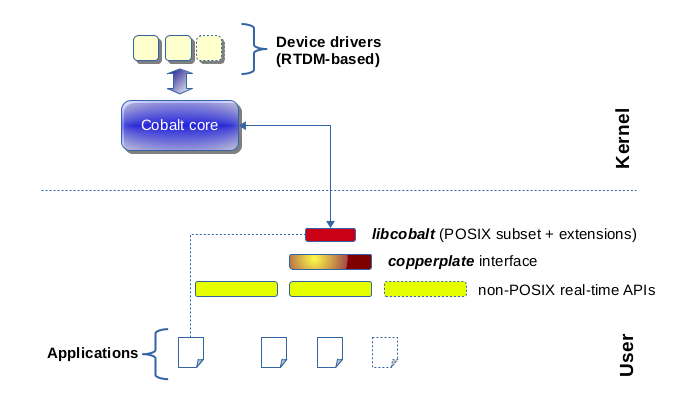
\includegraphics[width=0.6\columnwidth]{img/introduction/xenomai/x3-cobalt-interfaces.png}
	\caption[Xenomai 3 Cobalt Interfaces]{Xenomai 3 Cobalt Interfaces~\cite{OverviewXenomai}}
	\label{fig:cobalt}
\end{figure}

\noindent  The second approach, called Mercury and shown in Figure~\ref{fig:mercury}, relies on the real-time capabilities already present in the native Linux kernel. Often, applications require the PREEMPT-RT~\cite{RealtimePreempt_rt_versionsWiki} patch to augment the mainline kernel's real-time responsiveness and minimize jitter, but this is not mandatory and depends on the application's specific requirements for responsiveness and tolerance for occasional deadline misses.

\begin{figure}[H]
	\centering
	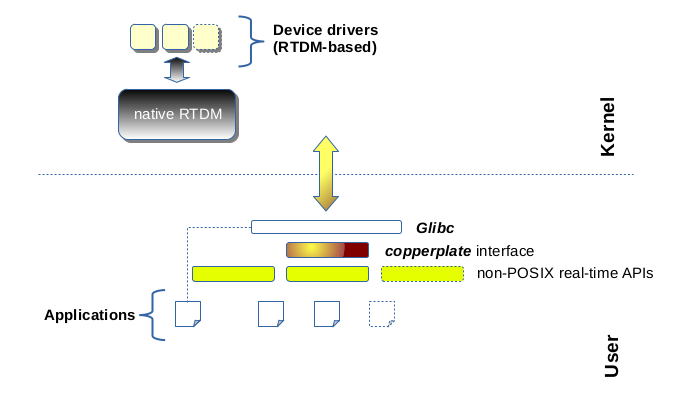
\includegraphics[width=0.6\columnwidth]{img/introduction/xenomai/x3-mercury-interfaces.png}
	\caption[Xenomai 3 Mercury Interfaces]{Xenomai 3 Mercury Interfaces~\cite{OverviewXenomai}}
	\label{fig:mercury}
\end{figure}

\noindent Salamander 4 uses the Cobalt real-time core with the Dovetail extension, which allows the kernel to handle real-time tasks with low latency. A key tool of the Xenomai suite that is used in this work is the \texttt{latency} tool~\cite{LATENCY}. It benchmarks the timer latency, which is the time it takes for the kernel to respond to timer interrupts or task activations. The tool creates real-time tasks or interrupt handlers and measures the difference between the expected and actual execution times.

\section{Trace-cmd}\label{sec:trace-cmd}
\texttt{Trace-cmd}~\cite{Tracecmd} is the front-end tool of the \texttt{ftrace} tool that is built inside the Linux kernel and used for tracing the Linux kernel. \texttt{Trace-cmd} can record detailed reports of kernel events such as interrupts, scheduler decisions, function calls, and custom events in real time. It is easier with this tool to enable and disable tracing, set filters, and view results. \texttt{Trace-cmd} helped debugging and identifying the reasons for latency in Salamander 4 to continuously improve its real-time performance and determinism. A very practical aspect of \texttt{trace-cmd} is that the guest can be traced from the host. For this purpose, the guest needs to be configured up with \texttt{vsocks}, which are a virtual socket that enable direct communication between the host and guest. To enable vsockets and tracing, the guest kernel requires the following configurations, according to Linux developer and maintainer Steve Rostedt~\cite{rostedtTracecmdHostGuest}.

\vspace{2em}
\begin{lstlisting}[language=bash, caption={Kernel Flags for Vsocks and Tracing}, label={lst:kernel-config}]
	# Vsockets settings
	CONFIG_VSOCKETS=m
	CONFIG_VHOST_VSOCK=m
	CONFIG_VIRTIO_VSOCKETS=m
	CONFIG_VIRTIO_VSOCKETS_COMMON=m
	CONFIG_VSOCKETS_DIAG=m
	CONFIG_VSOCKETS_LOOPBACK=m
	# Tracing settings
	CONFIG_TRACING=y
	CONFIG_FTRACE=y
	CONFIG_FUNCTION_TRACER=y
	CONFIG_FUNCTION_GRAPH_TRACER=y
	CONFIG_DYNAMIC_FTRACE=y
	CONFIG_DYNAMIC_FTRACE_WITH_REGS=y
	CONFIG_DYNAMIC_FTRACE_WITH_DIRECT_CALLS=y
	CONFIG_DYNAMIC_FTRACE_WITH_ARGS=y
	CONFIG_SCHED_TRACER=y
	CONFIG_FTRACE_SYSCALLS=y
	CONFIG_TRACER_SNAPSHOT=y
	CONFIG_KPROBE_EVENTS=y
	CONFIG_UPROBE_EVENTS=y
	CONFIG_BPF_EVENTS=y
	CONFIG_DYNAMIC_EVENTS=y
	CONFIG_PROBE_EVENTS=y
	CONFIG_SYNTH_EVENTS=y
	CONFIG_HIST_TRIGGERS=y
	\end{lstlisting}

\clearpage

\noindent After compiling the kernel with the additional settings aboce, the guest needs access to the vsocket. In QEMU, the line \texttt{-device vhost-vsock-pci,guest-cid=3,id=vsock0} was added. This command configures a virtual socket (vsock) device in QEMU, assigning the guest a unique Context Identifier (CID) of 3 for direct communication with the host. The CID can be chosen as desired. Once the guest is booted with vhost enabled, the \texttt{sudo trace-cmd agent} command can be run.  The agent now listens to connections on port 823 by default with the specified CID, 3 in this case. The host can trace itself and the guest from this moment going forward. For example, \texttt{sudo trace-cmd record -e all -A @3:823 --name Salamander4 -e all} records all events from the host and guest. \texttt{sudo trace-cmd record -e kvm:kvm\_entry -e kvm:kvm\_exit -A @3:823 --name Salamander4 -e all} traces onkly the \texttt{kvm\_entry} and \texttt{kvm\_exit} events of the host along with the exit reasons and all guest events. As a last example, \texttt{sudo trace-cmd record -e kvm -e sched -e irq -e -A @3:823 --name Salamander4 -e all} enables tracing of KVM, scheduling, and interrupt events on the host, for capturing the KVM events that manage the guest, scheduling activities, and interrupt handling respectively.

\section{Kernelshark}\label{sec:kernelshark}
Viewing the tracing data that was recorded with \texttt{trace-cmd} on a text-based file can be laborious. A better way of analyzing the data is done through \texttt{KernelShark}~\cite{KernelShark}, which is a graphical front-end tool. It visualizes the recorded kernel trace data in a readable way on an interactive timeline, which facilitates the process of identifying patterns and correlations between events. The latency issues can be analyzed by further filtering the displayed events according to processes, event types or time ranges. After the recording, \texttt{trace-cmd} gernerates a host \texttt{trace.dat} file and a guest \texttt{trace-Salamander4.dat} file, which in this case can be loaded into \texttt{KernelShark} with the command \texttt{kernelshark trace.dat -a trace-Salamander4.dat}. Once both files are loaded, the trace data can be visually inspected. All the current CPUs for both the host and the guest can be turned off, and the KVM Combo plots menu can be selected to view the guest vCPUs plotted on top of the host threads that run them, as depicted in Figure~\ref{fig:kernelshark_combo}.

\begin{figure}[H]
	\centering
	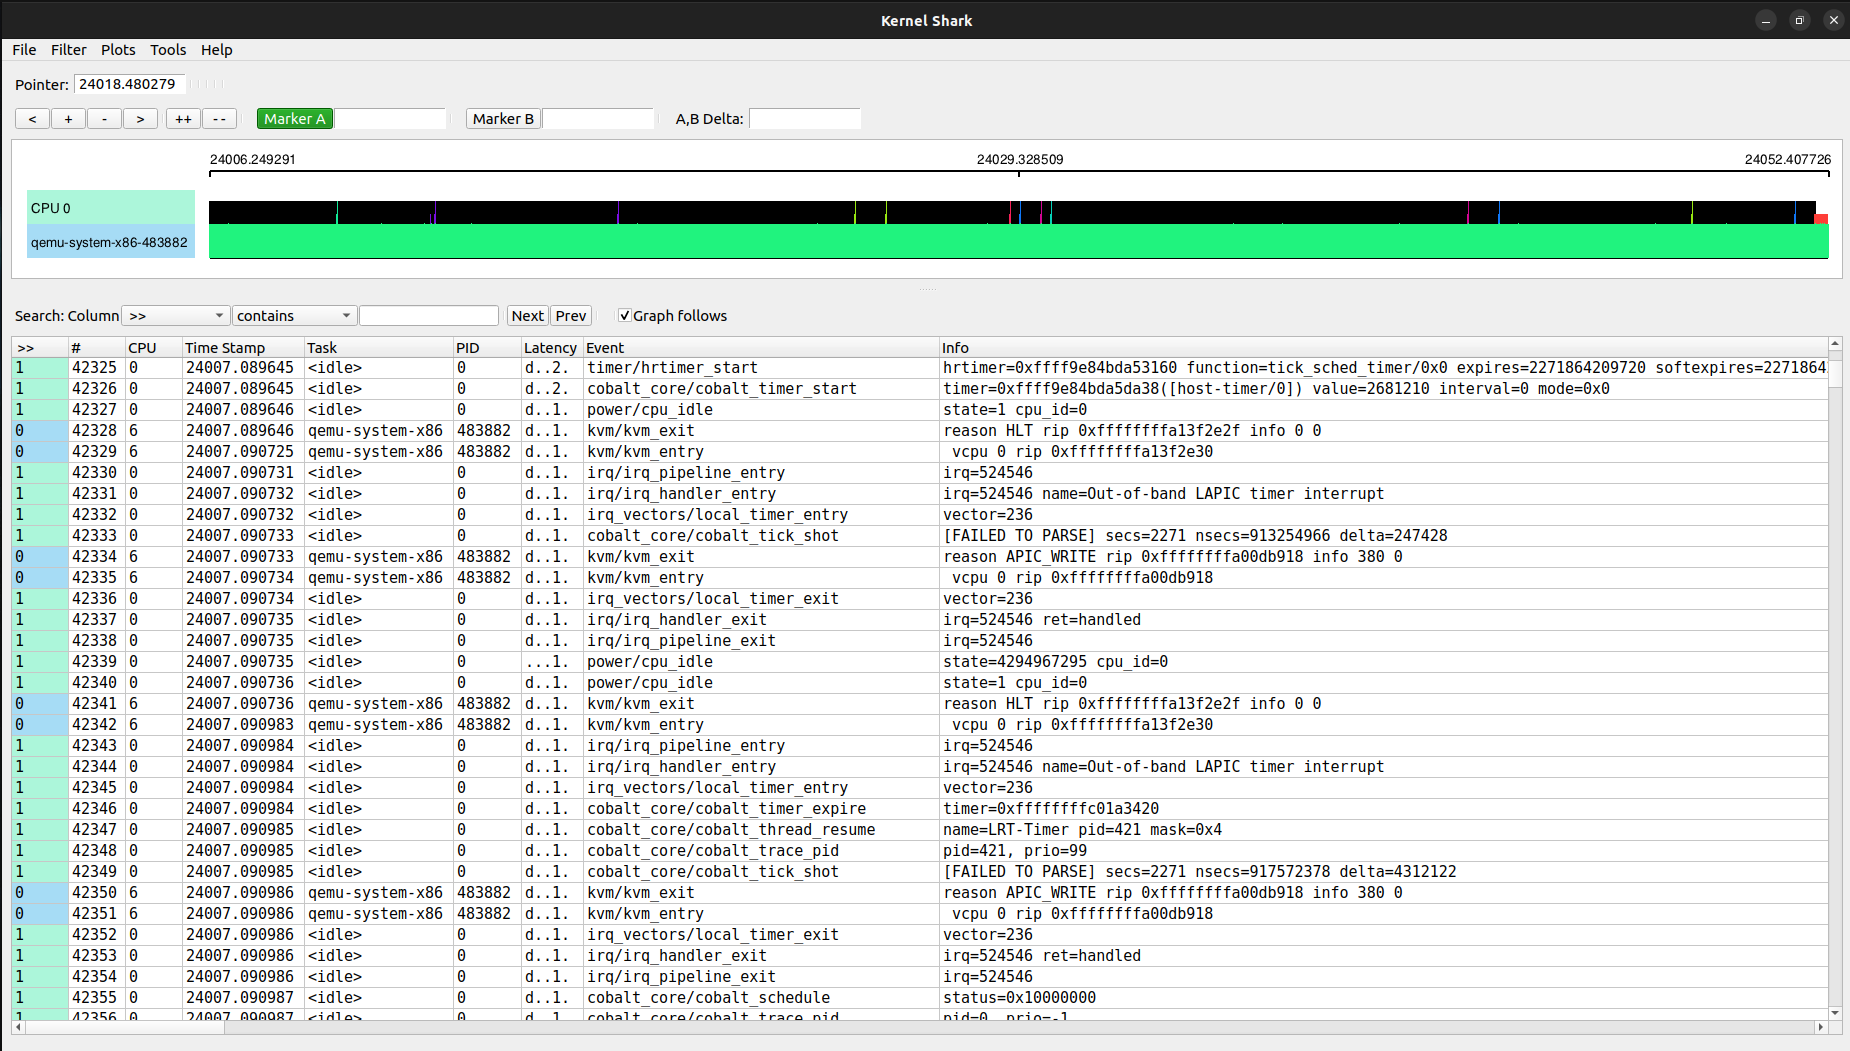
\includegraphics[width=1.0\columnwidth]{img/kernelshark_combo.png}
	\caption[Guest vCPUs plotted on top of Host Threads in KernelShark]{Guest vCPUs plotted on top of Host Threads in KernelShark}
	\label{fig:kernelshark_combo}
\end{figure}

\section{VARAN-Bus}\label{sec:varan}

VARAN is a real-time Ethernet bus designed for industrial automation, capable of connecting larger systems and machines with smaller components and sensors in hard real-time. This bus operates on the manager/client principle, where each network includes a manager and one or more subordinate clients. Multiple VARAN networks can be linked together into a single synchronized network using a higher-level VARAN manager. The jitter between these systems is kept below 100 ns. This synchronization between systens and their data exchange is illustrated in Figure~\ref{fig:multiple_varans}

\begin{figure}[H]
	\centering
	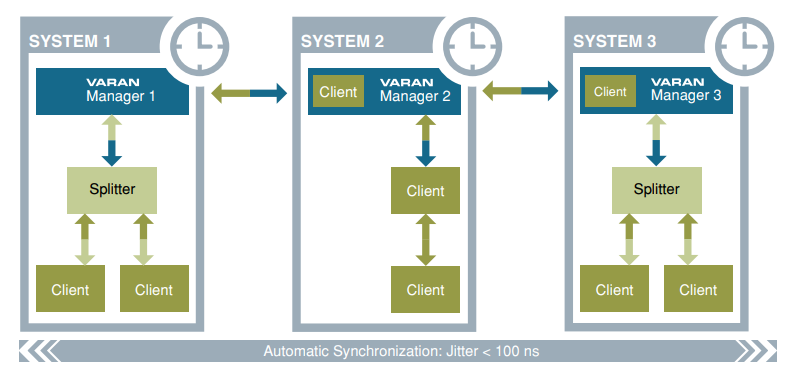
\includegraphics[width=0.75\columnwidth]{img/multiple_varans.png}
	\caption[Synchronization between Systems and their Data Exchange]{Synchronization between Systems and their Data Exchange}
	\label{fig:multiple_varans}
\end{figure}

\section{Approach}\label{sec:approach}
The goal is to The \texttt{latency} program is first executed in the bare metal Salamander 4 OS.
The goal is to virtualize the Salamander 4 OS and bring its real-time performance closer to that of the hardware version and guarantee deterministic and reliable behavior. For that purpose, the first step is to apply the PREEMPT-RT patch to the host system and subsequently tune the real-time performance through BIOS, kernel, host, guest and QEMU/KVM configurations. These modifications are added sequentially and tested together. First, the BIOS is configured, followed by the kernel. The BIOS settings are not reverted when moving to the kernel configurations. Next, the host is configured, but the BIOS and kernel settings remain unchanged. After that, the guest is configured, and finally, QEMU/KVM settings are applied. This means that the configurations are not isolated but are applied and then tested as a whole. The key metric here is the latency of the system, and the real-time performance is evaluated using the \texttt{latency} tool of the Xenomai suite after each configuration step. At the end, the results are domenstarted alltogether and a holistic comparison and discussion is carried out. In addition, the improvement in real-time performance and determinism is demonstrated using a robotic application, where the modified virtualization is compared with the hardware version.

\clearpage

\chapter{Implementation}

\section{Initial Situation}\label{sec:starting_situation}
As a starting point, initial latency values of both the bare metal and virtualization versions were measured with the \texttt{latency} tool of the Xenomai tool suite. Salamander 4 bare metal refers to the custom operating system developed by SIGMATEK, running on their proprietary hardware. Salamander 4 virtualization refers to a virtual version of Salamander 4, achieved through QEMU/KVM. Subsections~\ref{subsec:salamander4-bare-metal} and~\ref{subsec:salamander4-virtualization} specify the details of the measurements for both setups. In the further course of this master's thesis, the aim is to bring the latency values of the virtualization closer to those of the hardware and guarantee deterministic and reliable behavior.

\subsection{Salamander 4 Bare Metal}\label{subsec:salamander4-bare-metal}
As a reference point, the \texttt{latency} program was executed on Salamander 4 bare metal for a duration of 10 minutes. The complete command used was~\texttt{latency -h -g gnuplot.txt -T 600}, which runs the latency measurement tool for 600 seconds and prints histograms of minimum, average and maximum latencies in a Gnuplot-compatible format to the file~\texttt{gnuplot.txt}. Figure~\ref{fig:gnuplot_max_latency_hardware} depicts the distribution of latency over the course of said time.

\begin{figure}[H]
	\centering
	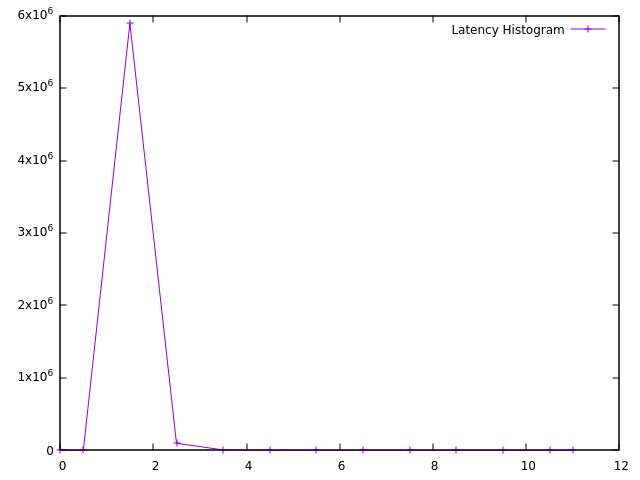
\includegraphics[width=0.7\columnwidth]{masterthesis-documentation/docs/sigmatek/xenomai/0hardware/gnuplot_max_latency_hardware.png}
	\caption[Latency Distribution of Salamander 4 Bare Metal]{Latency Distribution of Salamander 4 Bare Metal}
	\label{fig:gnuplot_max_latency_hardware}
\end{figure}

\noindent The statistics obtained from this measurement are provided in Table~\ref{tab:latency_stats_hardware} and Table~\ref{tab:latency_overrun_msw_hardware}. The test was conducted with a sampling period of 100 µs, using a periodic user-mode task, and was assigned a priority of 99. If any sample's latency value is greater than 100\textmu s, it would be considered an overrun.

\begin{table}[H]
	\centering
	\caption{Latency Parameters for Bare Metal}
	\label{tab:latency_stats_hardware}
	\begin{tabular}{|c|c|c|c|}
		\hline
		\textbf{Param} & \textbf{Samples} & \textbf{Average (µs)} & \textbf{Std Dev (µs)} \\ \hline
		\textbf{min}   & 599              & 0.711                 & 0.454                 \\ \hline
		\textbf{avg}   & 5 999 988        & 1.019                 & 0.150                 \\ \hline
		\textbf{max}   & 599              & 3.528                 & 0.895                 \\ \hline
	\end{tabular}
\end{table}

\begin{table}[H]
	\centering
	\caption{Minimum, Average, and Maximum Latency with Overrun Counts of Bare Metal}
	\label{tab:latency_overrun_msw_hardware}
	\begin{tabular}{|c|c|c|c|c|}
		\hline
		\textbf{Lat Min (µs)} & \textbf{Lat Avg (µs)} & \textbf{Lat Max (µs)} & \textbf{Overruns} \\ \hline
		0.613                 & 1.380                 & 10.709                & 0                 \\ \hline
	\end{tabular}
\end{table}

\subsection{Salamander 4 Virtualization}\label{subsec:salamander4-virtualization}
In addition to providing Salamander 4 on its own hardware, SIGMATEK has also developed a virtualised version of this operating system. Measuring the latency of the Salamander 4 virtualization with the default QEMU script in Code~\ref{script:qemu_def} and no further adjustments for 10 minutes, Figure~\ref{fig:gnuplot_max_latency_default} depicts the distribution of latency.

\begin{figure}[H]
	\centering
	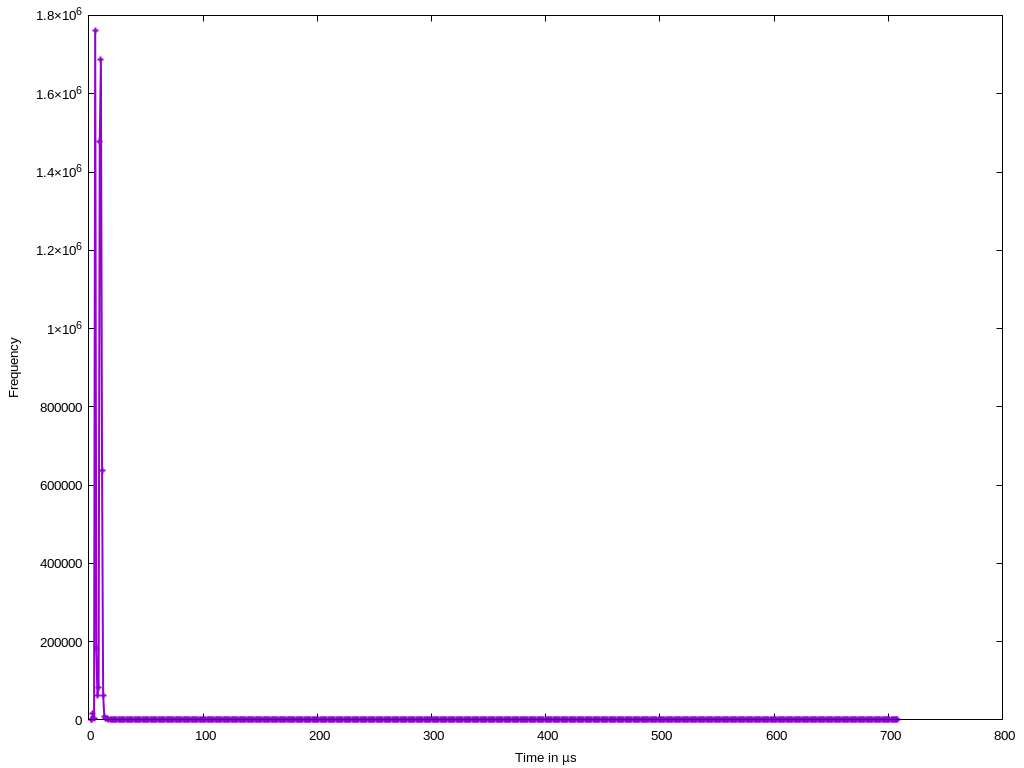
\includegraphics[width=0.7\columnwidth]{masterthesis-documentation/docs/sigmatek/xenomai/1default/gnuplot_max_latency_default.png}
	\caption[Latency Distribution of Salamander 4 Untuned Virtualization]{Latency Distribution of Salamander 4 Untuned Virtualization}
	\label{fig:gnuplot_max_latency_default}
\end{figure}

\noindent The statistics obtained from this measurement are provided in Table~\ref{tab:latency_stats_virt} and Table~\ref{tab:latency_overrun_msw_new_virt}. The test was again conducted with a sampling period of 100 µs, using a periodic user-mode task, and was assigned a priority of 99.

\begin{table}[H]
	\centering
	\caption{Latency Parameters for Untuned Virtualization}
	\label{tab:latency_stats_virt}
	\begin{tabular}{|c|c|c|c|}
		\hline
		\textbf{Param} & \textbf{Samples} & \textbf{Average (µs)} & \textbf{Std Dev (µs)} \\ \hline
		\textbf{min}   & 599              & 3.713                 & 1.355                 \\ \hline
		\textbf{avg}   & 5,999,922        & 8.247                 & 2.521                 \\ \hline
		\textbf{max}   & 599              & 45.705                & 52.196                \\ \hline
	\end{tabular}
\end{table}

\begin{table}[H]
	\centering
	\caption[Latency Statistics with Overrun Counts for Untuned Virtualization]{Minimum, Average, and Maximum Latency with Overrun Counts for Untuned Virtualization}
	\label{tab:latency_overrun_msw_new_virt}
	\begin{tabular}{|c|c|c|c|c|}
		\hline
		\textbf{Lat Min (µs)} & \textbf{Lat Avg (µs)} & \textbf{Lat Max (µs)} & \textbf{Overruns} \\ \hline
		2.536                 & 8.940                 & 707.622               & 43                \\ \hline
	\end{tabular}
\end{table}

\subsection{Initial Comparison}
\noindent Comparing the latency values of the virtualization to those of bare metal in Figure~\ref{fig:gnuplot_max_latency_combined}, it is evident that there is a significant initial gap in the statistics. A maximum latency of 707.62~\textmu s is not tolerable for a real-time virtualization and needs to be tuned.

\begin{figure}[H]
	\centering
	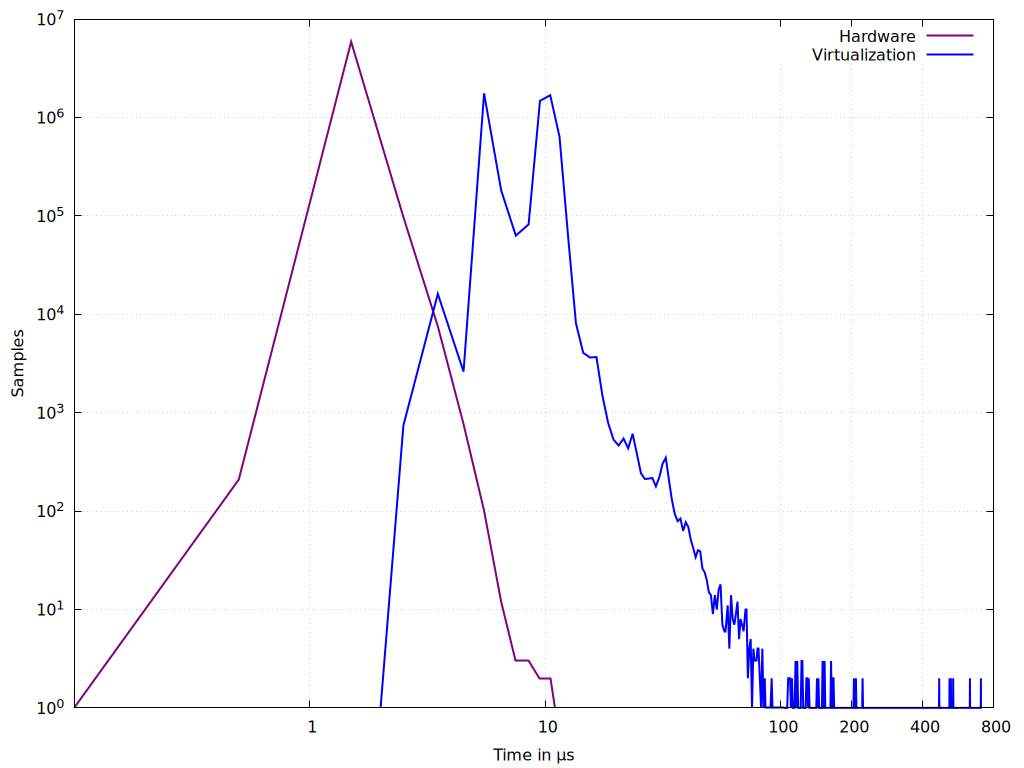
\includegraphics[width=0.7\columnwidth]{masterthesis-documentation/docs/sigmatek/xenomai/01combined/gnuplot_combined_max_latency.png}
	\caption[Initial Comparison of Latency Distribution between Hardware and Virtualization]{Initial Comparison of Latency Distribution between Hardware and Virtualization}
	\label{fig:gnuplot_max_latency_combined}
\end{figure}

\clearpage

\section{Real-Time Performance Tunings}\label{sec:real-time_tunings}

In this chapter, the significant initial gap in latency statistics between the virtualized system and the bare metal system is tackled. For this reason, an extensive tuning process is carried out. This involves configurations spanning the BIOS, kernel, host OS, QEMU/KVM virtualization layer, and the Salamander 4 OS itself. The individual configurations are discussed in detail and the modifications are justified with a clear explanation. The goal is to bring the latency of the virtualization closer to that of the bare metal, thereby ensuring deterministic behavior under real-time constraints.

\bigskip \noindent It is important to mention that a real-time system implies determinism at every component of the system, ranging from hardware over the kernel to the software and the application on it. As already established earlier, the guest OS Salamamder 4 runs Xenomai and is hence real-time capable. The host system also needs to be aware of the real-time determinism in order to achieve highest possible reliability. The very step of achieving the goal of reducing latency is to apply the PREEMPT-RT patch to the host system. This patch is a set of modifications to the Linux kernel with the goal of making it fully preemptible. This means, almost all parts of the kernel can be preempted and higher-priority tasks can interrupt lower-priority ones. This significantly reduces the time it takes for high-priority tasks to start executing after an event~\cite{RealtimeKernelPatchset}. The patch also includes support for high-resolution timers and makes the system more predictable~\cite{lutsykPipelinedMulticoreMachine2020}. Determinism and predictability are key for real-time applications where the timing of operations must be guaranteed with precise timing and scheduling~\cite{rostedtInternalsRTPatch2007}.

\bigskip \noindent Nevertheless, a real-time kernel alone does not make a system truly “real-time”~\cite{WhatRealtimeLinuxa}. Additional modifications are required to achieve this. The next sections will deal with these real-time performance tunings. After each tuning, the \texttt{latency} test of Xenomai is executed to evaluate the improved latency. The most important metric of a latency test is without a doubt the worst latency value, because the system is only as reliable as its worst measurement. Since the period of the tests is set to 100\textmu s, there are approximately 1,000,000 samples per second.

\clearpage

\subsection{BIOS Configurations}\label{subsec:bios_configurations}

BIOS stands for Basic Input/Output System. It abstracts the hardware and enables basic functions of a computer during the booting process, such as starting the operating system and loading other software. Since the BIOS is embedded very deep, its configuration can significantly influence the real-time performance of the system. Table~\ref{tab:bios_configuration} illustrates the specific BIOS settings that have been adjusted for the purpose of real-time performance. As an important note, this is not a definitive, full-ended list, and other devices may have additional settings that can be modified to achieve even better latency.

\begin{table}[H]
	\centering
	\caption{BIOS Configurations for Real-Time Performance}
	\label{tab:bios_configuration}
	\setlength{\tabcolsep}{0.5em} % for the horizontal padding
	{\renewcommand{\arraystretch}{1.2}% for the vertical padding
		\begin{tabular}{|l|l|}
			\hline
			\textbf{Option}               & \textbf{Status} \\
			\hline
			Hyper Threading               & Disabled        \\
			\hline
			Intel SpeedStep®              & Disabled        \\
			\hline
			Intel® Speed Shift Technology & Disabled        \\
			\hline
			C States                      & Disabled        \\
			\hline
			VT-d                          & Enabled         \\
			\hline
		\end{tabular}}
\end{table}

\noindent In the following, these settings along with their impact on system latency are briefly described.

\begin{itemize}
	\item \textbf{Hyper Threading}: When hyper-threading is enabled in thd BIOS settings, this allows CPUs to work on two threads simultaneously instead of just one. This allows the parallelisation of tasks and seemingly increases performance. However, in a real-time system like the guest Salamander 4, this can lead to increased latencies due to contention between threads. In order to ensure more deterministic behavior in the guest, it is disabled on the host.
	\item \textbf{Intel SpeedStep}: This dynamically adjusts the clock speed of the CPU based on workload. These dynamic adjustments of the speed can lead to unpredictable latencies in a real-time system. It is also disabled on the host to maintain a constant CPU speed.
	\item \textbf{Intel® Speed Shift Technology}: Similar to SpeedStep, Speed Shift allows the processor to directly control its frequency and voltage. This can lead to unpredictable latencies, too. Hence, it is also disabled on the host.
	\item \textbf{C States}: These are low-power idle states where the clock frequency and voltage of the CPU are reduced. Transitioning between C-states can cause variable latencies. To prevent this from happening, C-states are disabled on the host.
	\item \textbf{VT-d}: Direct access to physical devices from within virtual machines is possible when VT-d is enabled on the host. This can help reduce latencies associated with I/O operations in the virtual machine. It is therefore enabled on the host.
\end{itemize}

\noindent After these first real-time tunings in the BIOS settings, the \texttt{latency} test was run to see, whether this had any significant impact on the determinism of the system. Figure~\ref{fig:gnuplot_max_latency_taskset} shows the latency values after tuning BIOS settings.

\begin{figure}[H]
	\centering
	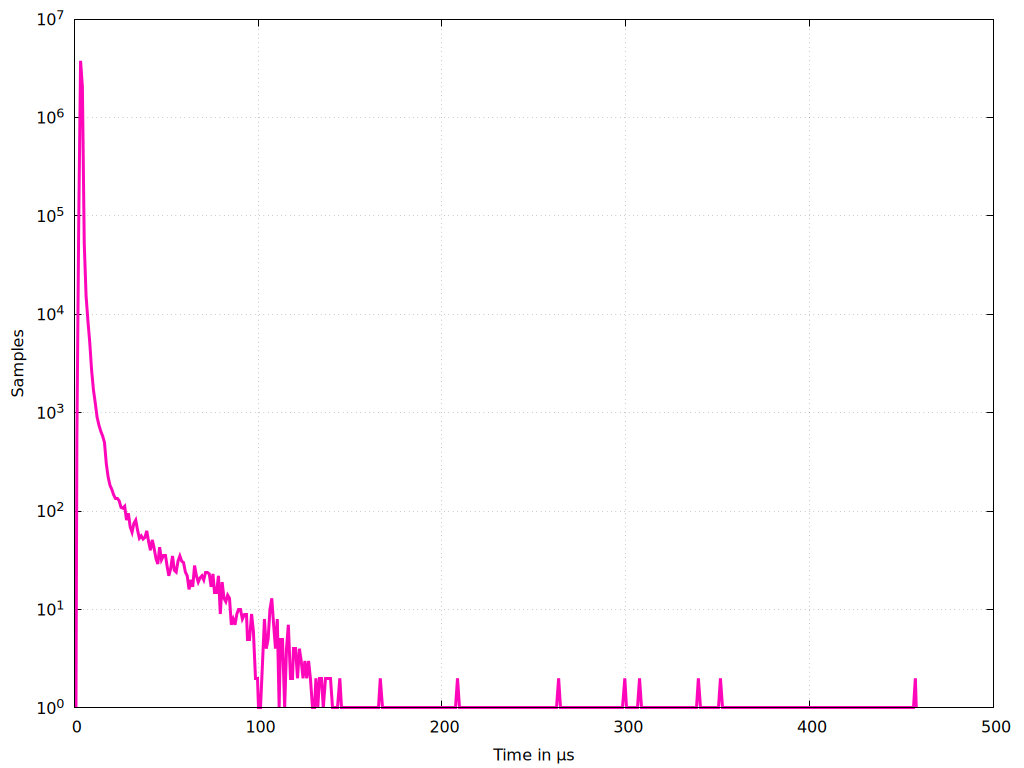
\includegraphics[width=0.7\columnwidth]{masterthesis-documentation/docs/sigmatek/xenomai/2taskset/gnuplot_max_latency_taskset.png}
	\caption[Latency Distribution of Salamander 4 after BIOS Configurations]{Latency Distribution of Salamander 4 Virtualization after tuning BIOS Configurations}
	\label{fig:gnuplot_max_latency_taskset}
\end{figure}

\noindent The statistics obtained from this measurement are provided in Table~\ref{tab:latency_stats_virt} and Table~\ref{tab:latency_overrun_msw_new_virt}.

\begin{table}[H]
	\centering
	\caption{Latency Parameters after BIOS Configurations}
	\label{tab:latency_stats_virt_bios}
	\begin{tabular}{|c|c|c|c|}
		\hline
		\textbf{Param} & \textbf{Samples} & \textbf{Average (µs)} & \textbf{Std Dev (µs)} \\ \hline
		\textbf{min}   & 599              & 1.419                 & 0.507                 \\ \hline
		\textbf{avg}   & 5,999,885        & 3.398                 & 1.251                 \\ \hline
		\textbf{max}   & 599              & 74.015                & 26.590                \\ \hline
	\end{tabular}
\end{table}

\begin{table}[H]
	\centering
	\caption[Latency Statistics with Overrun Counts after BIOS Configurations]{Minimum, Average, and Maximum Latency with Overrun Counts after BIOS Configurations}
	\label{tab:latency_overrun_msw_new_virt_bios}
	\begin{tabular}{|c|c|c|c|c|}
		\hline
		\textbf{Lat Min (µs)} & \textbf{Lat Avg (µs)} & \textbf{Lat Max (µs)} & \textbf{Overruns} \\ \hline
		0.969                 & 3.948                 & 457.545               & 94                \\ \hline
	\end{tabular}
\end{table}

\noindent The maximum latency value recorded was 457.545\textmu s. When compared to the inital worst latency of 707.62 \textmu s, this is a step for the better, but certainly still not acceptable within this work's definition of hard real-time determinism.

\subsection{Kernel Configurations}\label{subsec:kernel_configurations}
The kernel command-line parameters are shown in Code~\ref{script:kernel_cli} below. To access and modify them, the file is located in \texttt{/etc/default/grub}.

\vspace{2em}
\begin{lstlisting}[name={Kernel Configurations for Real-Time Performance},label={script:kernel_cli}]
		GRUB_CMDLINE_LINUX="isolcpus=4 rcu_nocbs=4 rcu_nocb_poll nohz_full=4 nohz=on default_hugepagesz=1G hugepagesz=1G hugepages=8 intel_iommu=on rdt=l3cat nmi_watchdog=0 idle=poll clocksource=tsc tsc=reliable audit=0 skew_tick=1 intel_pstate=disable intel.max_cstate=0 intel_idle.max_cstate=0 processor.max_cstate=0 processor_idle.max_cstate=0 nosoftlockup no_timer_check nospectre_v2 spectre_v2_user=off kvm.kvmclock_periodic_sync=N kvm_intel.ple_gap=0 irqaffinity=0"
\end{lstlisting}

\noindent In the following, these settings along with their impact on system latency are briefly described.

\begin{itemize}
	\item \textbf{isolcpus=4}: Isolates CPU 4 from the general scheduler, meaning no process will be scheduled to run on this CPU unless it is explicitly assigned. CPU isolation is explained in detail in Subsubsection~\ref{subsubsec:cpu_isolation}.
	\item \textbf{rcu\_nocbs=4}: The Linux kernel uses a synchronization mechanism called RCU, or Read-Copy-Update. It lets writers update the data in a way that guarantees readers will always see the same version while enabling multiple readers to access shared data without locks. The RCU subsystem uses callback functions that need to be invoked once readers are done with the data they accessed. By default, these callbacks are handled by the CPUs that executed the read-side critical sections. This parameter offloads RCU callback handling from CPU 4 to other CPUs. CPU 4 remains dedicated to high-priority tasks which helps in reducing latency.
	\item \textbf{rcu\_nocb\_poll}: This is used together with \texttt{rcu\_nocbs} and causes the system to actively poll for RCU callbacks to invoke, instead of waiting for the next RCU grace period. This reduces latency.
	\item \textbf{nohz\_full=4}: Makes CPU core 4 ``tickless'', meaning the kernel tries to avoid sending periodic scheduling-clock interrupts to the CPU when there are no runnable tasks. This lowers latency by reducing unnecessary wake-ups but may increase power consumption because the CPU is not able to enter a low-power state when idle. Additionally, timer interrupts cannot be fully eliminated because certain events, such as incoming interrupts or task activations, can still cause the kernel to send timer interrupts to the tickless CPU.
	\item \textbf{nohz=on}: Sets all CPUs to tickless mode system-wide.
	\item \textbf{default\_hugepagesz=1G, hugepagesz=1G, hugepages=8}: Huge pages are large contiguous areas of memory that can be used by applications and the kernel, instead of the traditional 4KB small pages. The default huge page size is set to 1GB, and 8 huge pages of 1GB size are reserved at boot. This pre-allocation makes sure that these large memory regions are available to be used by the kernel or applications, without having to dynamically allocate and potentially fail.
	\item \textbf{intel\_iommu=on}: Enables Intel's IOMMU (Input/Output Memory Management Unit), which connects a DMA (Direct Memory Access)-capable I/O bus, such as graphics cards and network adapters, to the main memory. It allows these devices to directly access and use memory, which is especially helpful when they are virtualized.
	\item \textbf{rdt=l3cat}: Activates the L3 CAT (L3 Cache Allocation Technology) feature of Intel’s RDT (Resource Director Technology). Unlike L1 and L2 caches, where each core has its fixed capacity, L3 cache is a shared pool among multiple cores. L3 CAT controls the amount of L3 cache that a process can use. By controlling cache allocation, it can prevent a single process from monopolizing the L3 cache, which is particularly beneficial in virtualized environments, where multiple virtual machines share the same physical host.
	\item \textbf{nmi\_watchdog=0}: Disables the NMI (Non-Maskable Interrupt) watchdog, which is a debugging feature of the Linux kernel. It works by periodically generating non-maskable interrupts. If the system does not respond to these interrupts within a certain timeframe, the NMI watchdog concludes that the system has hung and generates a system dump for debugging.  This constant monitoring consumes CPU cycles and can introduce undesirable latency in real-time systems.
	\item \textbf{idle=poll}: Changes the CPU’s idle loop behavior to active polling. Instead of entering a low-power state when idle, the CPU continuously polls for new tasks. This can reduce task start latency in real-time systems, but it increases power consumption.
	\item \textbf{clocksource=tsc, tsc=reliable}: TSC (Time Stamp Counter) is a high-resolution timer provided by most x86 processors that counts the number of CPU cycles since it was last reset. Accurate timekeeping is crucial, particularly for real-time systems. These parameters set the clocksource to TSC and mark it as a reliable source of timekeeping, meaning it increments at a consistent rate and does not stop when the processor is idle.
	\item \textbf{audit=0}: Disables the Linux audit system. When it is enabled, it generates log entries for security-relevant events, which is a slow operation since they are written to disk. If there are a large number of such events, the audit system can consume significant CPU time and I/O bandwidth which could lead to higher latency.
	\item \textbf{skew\_tick=1}: Enables a mode in the Linux kernel that reduces timer interrupt overhead. Normally, timer interrupts happen simultaneously on all CPUs, resulting in all CPUs to exit their low-power states at once. This can lead to increased contention for system resources. When enabled, the kernel offsets the timer interrupts on different CPUs, spreading them out over time.
	\item \textbf{intel\_pstate=disable}: Disables the Intel P-state driver, which is a part of the Linux kernel that handles power management for Intel CPUs. It controls the frequency of the CPU by scaling it up when demand is high and scaling it down to save power when demand is low. This dynamic frequency scaling is disabled because it leads to increased latencies for real-time systems.
	\item \textbf{intel.max\_cstate=0, intel\_idle.max\_cstate=0, processor.max\_cstate=0, processor\_idle.max\_cstate=0}: These parameters disable deeper C-states (CPU power saving states). Normally, when a CPU is idle, it can enter various C-states, with higher-numbered states representing deeper sleep states that save more power but take longer to wake up from. In real-time systems, these wake-up delays can be problematic. Disabling them leads keeps the CPUs ready to respond quickly to new tasks and helps in reducing latency.
	\item \textbf{nosoftlockup}: Disables the soft lockup detector in the Linux kernel. A soft lockup is when a CPU is busy executing kernel code for a long period of time without giving other tasks a chance to run. Especially threads with SCHED\_FIFO policy occupy the CPU for an extensive duration. This is detected and reported by the soft lockup detector, hence it is disabled to prevent these unnecessary warnings.
	\item \textbf{no\_timer\_check}: Disables the check for broken timer interrupt sources. Broken timer interrupt sources are problems with hardware or software that prevent timer interrupts from working as intended. Such a timer may not generate interrupts at the expected rate or at all. The kernel skips the checks for these broken timer interrupt sources, which can cause unnecessary overhead in a real-time system where every CPU cycle counts.
	\item \textbf{nospectre\_v2, spectre\_v2\_user=off}: These parameters disable mitigations for the Spectre v2 vulnerability. Spectre v2 is a hardware vulnerability that affects many modern microprocessors and can allow malicious programs to access sensitive data they are not supposed to. While this is necessary for security, it has an impact on performance and should be turned off in controlled environments where the risk of exploitation is low.
	\item \textbf{kvm.kvmclock\_periodic\_sync=N, kvm\_intel.ple\_gap=0}: These are KVM (Kernel-based Virtual Machine) related parameters. They disable the periodic synchronization of the kvmclock and set the gap between PLE (Pause Loop Exiting) events to 0. The kvmclock is a paravirtualized clock source provided by KVM to its guest OS and disabling this reduces latency introduced by clock synchronization. By setting the gap to 0, the virtual machine exits the pause loop immediately, which can reduce latency in spinlock-intensive workloads.
	\item \textbf{irqaffinity=0}: Sets the default interrupt request affinity to none. This means that no CPU core is preferred over another for handling IRQs. Instead, it lets the operating system decide how to distribute these IRQs across all the CPUs. Subsubsection~\ref{subsubsec:irq_handling} dives deeper into interrupt request affinity.
\end{itemize}

\clearpage

\noindent After the kernel modifications on top of the BIOS settings from the last subsection, Figure~\ref{fig:gnuplot_max_latency_rt_kernelparam} demonstrates the latency
values gathered in 10 minutes.

\begin{figure}[H]
	\centering
	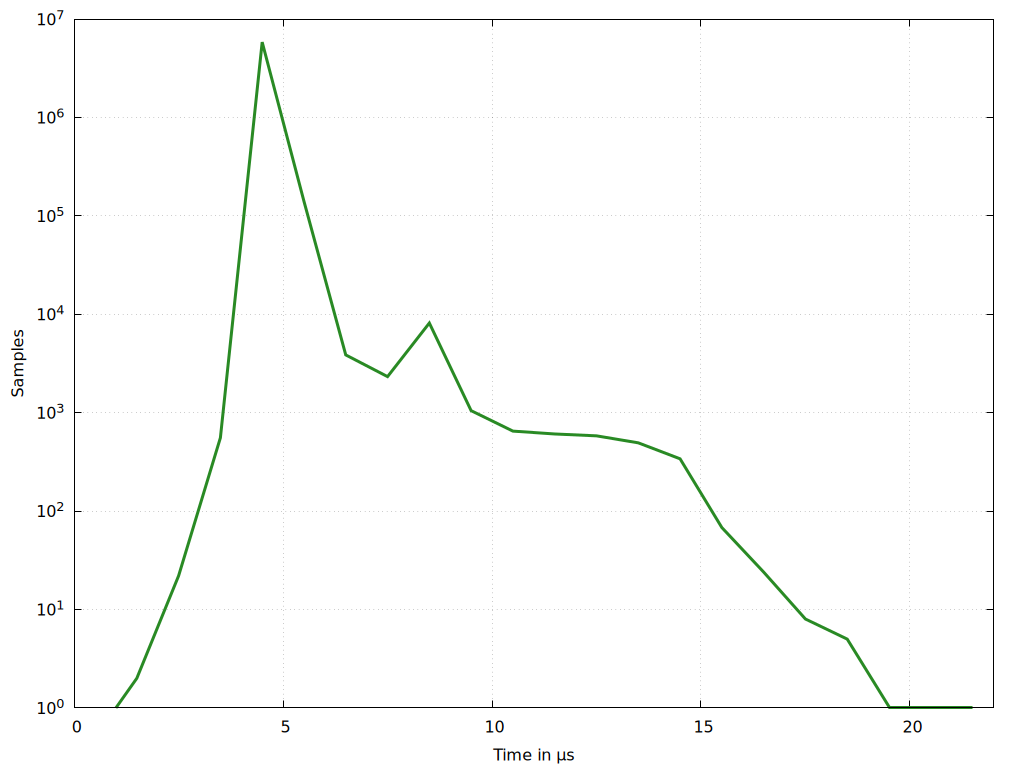
\includegraphics[width=0.7\columnwidth]{masterthesis-documentation/docs/sigmatek/xenomai/4rt_kernelparam/gnuplot_max_latency_rt_kernelparam.png}
	\caption[Latency Distribution of Salamander 4 after Kernel Configurations]{Latency Distribution of Salamander 4 Virtualization after tuning Kernel Configurations}
	\label{fig:gnuplot_max_latency_rt_kernelparam}
\end{figure}

\noindent The statistics obtained from this measurement are provided in Table~\ref{tab:latency_stats_kernelparam} and Table~\ref{tab:latency_overrun_msw_new_virt_kernel}.

\begin{table}[H]
	\centering
	\caption{Latency Parameters after Kernel Configurations}
	\label{tab:latency_stats_kernelparam}
	\begin{tabular}{|c|c|c|c|}
		\hline
		\textbf{Param} & \textbf{Samples} & \textbf{Average (µs)} & \textbf{Std Dev (µs)} \\ \hline
		\textbf{min}   & 599              & 3.356                 & 0.551                 \\ \hline
		\textbf{avg}   & 5,999,972        & 4.036                 & 0.290                 \\ \hline
		\textbf{max}   & 599              & 13.484                & 1.454                 \\ \hline
	\end{tabular}
\end{table}

\begin{table}[H]
	\centering
	\caption[Latency Statistics with Overrun Counts after Kernel Configurations]{Minimum, Average, and Maximum Latency with Overrun Counts after Kernel Configurations}
	\label{tab:latency_overrun_msw_new_virt_kernel}
	\begin{tabular}{|c|c|c|c|c|}
		\hline
		\textbf{Lat Min (µs)} & \textbf{Lat Avg (µs)} & \textbf{Lat Max (µs)} & \textbf{Overruns} \\ \hline
		2.545                 & 4.811                 & 21.694                & 0                 \\ \hline
	\end{tabular}
\end{table}

\noindent Apparent is a significant improvement in the latency of the virtualized Salamander 4 OS. With a worst latency value of 21.694\textmu s, the real-time tunings appear to be working as desired.

\clearpage

\subsection{Host OS Configurations}\label{subsec:host_configurations}
The host OS needs to provide an environment where the guest OS can operate in real-time. This entails a number of host-side adjustments to reduce interruptions and latency. In the following, a detailed overview of these configurations and their impact on the real-time performance of the guest Salamander 4 OS is provided.
\subsubsection{CPU affinity and Isolation}\label{subsubsec:cpu_isolation}

Isolating CPUs means removing all user-space threads and unbound kernel threads, since bound kernel threads are tied to specific CPUs and hence cannot be moved. For CPU isolation, the~\texttt{isolcpus} function is used to isolate a performance CPU from the general scheduling algorithms of the operating system. This means that the isolated CPUs will not be used for regular task scheduling, allowing them to be dedicated for the real-time specific tasks. However, the isolcpus function only isolates at the user level and does not affect kernel tasks. Consequently, these kernel tasks and interrupts can still utilize the CPU~\cite{maPerformanceTuningKVMbased2013}, including systemd services. To prevent systemd services from running on an isolated CPU, the CPU affinity can be set with the line \texttt{CPUAffinity=0 1 2 3 5} in the \texttt{/etc/systemd/system.conf} file to indicate the CPUs that systemd services are allowed to run on. Every CPU other than the isolated CPU 4 is allowed. Code~\ref{output:pse} shows the user and kernel tasks that run on CPU 4. An isolated CPU can be bound to a task by using \texttt{taskset -c <CPU>}, as shown later in Subsection~\ref{subsec:guest_configurations}. After the isolation, user tasks other than the QEMU process have been removed from running on this CPU. Only few per-CPU kernel threads that are tied to this CPU still take CPU time.

\vspace{2em}
\begin{lstlisting}[name={User and Kernel Tasks on the isolated CPU},label={output:pse},escapeinside={(*@}{@*)}]
		sigma_ibo@sigma-ibo:~$ cat /sys/devices/system/cpu/isolated
		4
		sigma_ibo@sigma-ibo:~$ ps axHo psr,pid,lwp,args,policy,nice,rtprio | awk '$1 == 4'
		4      38      38 [cpuhp/4]                   TS    0      -
		4      39      39 [idle_inject/4]             FF    -     50
		4      40      40 [migration/4]               FF    -     99
		4      41      41 [ksoftirqd/4]               TS    0      -
		4      42      42 [kworker/4:0-events]        TS    0      -
		4      43      43 [kworker/4:0H-kblockd]      TS  -20      -
		4     153     153 [kworker/4:1-events]        TS    0      -
		4   81649   81649 qemu-system-x86_64 -M pc,ac TS    0      -
		4   81649   81654 qemu-system-x86_64 -M pc,ac TS    0      -
		4   81649   81676 qemu-system-x86_64 -M pc,ac TS    0      -
		4   81649   81702 qemu-system-x86_64 -M pc,ac TS    0      -
		4   81649   82185 qemu-system-x86_64 -M pc,ac TS    0      -
		4   81649   82187 qemu-system-x86_64 -M pc,ac TS    0      -
		4   82134   82134 [kworker/4:1H-kblockd]      TS  -20      -
\end{lstlisting}

\subsubsection{Interrupt Affinity}\label{subsubsec:irq_handling}
Once the CPUs were isolated, interrupt requests handling was the next step. The purpose of interrupt requests is to inform the CPU to stop working on a certain job and start working on another. This allows hardware devices to communicate with the CPU through frequent context switches, which can introduce latency in real-time systems. All the existing interrupts can be monitored using the command~\texttt{watch -d -n 1 cat /proc/interrupts} to observe changes in the interrupt requests handled by each CPU in real-time. The IRQs needed to be removed from the isolated CPU by manipulating the~\texttt{/proc/irq/<IRQ>/smp\_affinity} files. The value in the~\texttt{smp\_affinity} file is a bitmask in hexadecimal format where each bit corresponds to a CPU. The least significant bit (LSB) on the right corresponds to the first CPU (CPU0), and the most significant bit (MSB) on the left corresponds to the last CPU (CPU5). When there are 6 CPUs available, the default value for~\texttt{smp\_affinity} would be 3F (11 1111). Removing CPU 4 out of this bitmask would be setting bit five to zero, resulting in 2F (10 1111). The python script in Code~\ref{script:smp_affinity} was written to show a table of the distribution of interrupt requests across each CPU, since the \texttt{/proc/interrupts} file does not give away this information and looking individually in the \texttt{/proc/irq/<IRQ>/smp\_affinity} files for every IRQ would be time-consuming. The program first reads the CPU affinity settings for each IRQ from the \texttt{/proc/irq} directory and stores the CPUs assigned to each IRQ in a dictionary. It then creates a data frame to represent this information in a table format, marking the assigned CPUs with ‘x’. Finally, it prints the table and saves it as a markdown file.

\bigskip \noindent However, as the \texttt{proc} filesystem resets to its default state after each reboot, manually changing numerous IRQ files through the said bitbasks is tedious and time-consuming. This process can be was automated using the shell script in Code~\ref{script:change_smp_affinity}, which can automatically be executed after every reboot.

\bigskip \noindent Additionally, the CPU affinity of IRQ threads of NVME (Non-Volatile Memory Express, a type of SSD storage) can be set away from CPU 4 to avoid impacting real-time workloads. This can be done through finding out the respective process IDs through \texttt{ps -e | grep irq/.*nvme} and then executing \texttt{sudo taskset -a -p -c 0 <PID>}.

\clearpage

\vspace*{-5em}
\begin{lstlisting}[name={Code to show a table of the distribution of interrupt requests across each CPU},label={script:smp_affinity}]
		import os
		import pandas as pd
		from tabulate import tabulate
		
		# Get the number of CPUs
		num_cpus = os.cpu_count()
		
		# Initialize a dictionary to store the CPUs for each IRQ
		irqs = {}
		
		# Iterate over each IRQ
		for irq in os.listdir('/proc/irq'):
			# Check if the smp_affinity file exists for this IRQ
			if os.path.isfile(f'/proc/irq/{irq}/smp_affinity'):
				# Read the current smp_affinity
				with open(f'/proc/irq/{irq}/smp_affinity', 'r') as f:
					affinity = int(f.read().strip(), 16)
				# Initialize an empty list to store the CPUs for this IRQ
				cpus = []
				# Iterate over each CPU
				for cpu in range(num_cpus):
					# Check if the bit for the current CPU is set
					if ((affinity & (1 << cpu)) != 0):
						# Add the CPU to the list for this IRQ
						cpus.append(cpu)
				# Sort the list of CPUs
				cpus.sort()
				# Add the list of CPUs to the dictionary for this IRQ
				irqs[irq] = cpus
		
		# Create a DataFrame to store the table
		df = pd.DataFrame(index=sorted(irqs.keys(), key=int), columns=range(num_cpus))
		
		# Fill the DataFrame with 'x' where a CPU is assigned to an IRQ
		for irq, cpus in irqs.items():
			for cpu in cpus:
				df.loc[irq, cpu] = 'x'
		
		# Replace NaN values with empty strings
		df.fillna('', inplace=True)
		
		# Print the table in pipe format
		print(tabulate(df, headers='keys', tablefmt='pipe', showindex=True))
		
		# Convert the DataFrame to a markdown table
		markdown_table = df.to_markdown()
		
		# Write the markdown table to a file
		with open('table_CPU_IRQ.md', 'w') as f:
			f.write(markdown_table)
\end{lstlisting}

\clearpage

\vspace*{-5em}
\begin{lstlisting}[name={Script to change IRQ Assignment of a CPU},label={script:change_smp_affinity}]
		#!/bin/bash

		# Check if a command-line argument is provided
		if [ -z "$1" ]; then
			echo "Please provide a CPU number as a command-line argument."
			exit 1
		fi
		
		# Get the CPU number from the command-line argument
		CPU=$1
		
		# Define the mask values
		declare -A mask_values
		mask_values=( [0]="3ffe" [1]="3ffd" [2]="3ffb" [3]="3ff7" [4]="3fef" [5]="3fdf" [6]="3fbf" [7]="3f7f" [8]="3eff" [9]="3dff" [10]="3bff" [11]="37ff" [12]="2fff" [13]="17ff")
		
		# Run the check_smp_affinity.sh script and get the IRQs
		IRQs=$(./check_smp_affinity.sh $CPU | grep -o '[0-9]\+')
		
		# Initialize an empty array to store the IRQs that could not be removed
		failed_IRQs=()
		# Initialize an empty array to store the IRQs that were successfully removed
		succeeded_IRQs=()
		
		# Loop over the IRQs
		for IRQ in $IRQs; do
			# Try to change the smp_affinity
			echo ${mask_values[$CPU]} | sudo tee /proc/irq/$IRQ/smp_affinity > /dev/null 2>&1
			# If the command failed, add the IRQ to the failed_IRQs array
			if [ $? -ne 0 ]; then
				failed_IRQs+=($IRQ)
			else
				succeeded_IRQs+=($IRQ)
			fi
		done
		
		# Check if there were any failed IRQs
		if [ ${#failed_IRQs[@]} -ne 0 ]; then
			echo "IRQs ${failed_IRQs[@]} could not be removed from CPU $CPU."
		fi
		
		# Check if there were any successful IRQs
		if [ ${#succeeded_IRQs[@]} -ne 0 ]; then
			# Remove the first entry from the succeeded_IRQs array
			succeeded_IRQs=("${succeeded_IRQs[@]:1}")
			echo "IRQs ${succeeded_IRQs[@]} were removed from CPU $CPU."
		fi		
\end{lstlisting}

\subsubsection{RT-Priority}
Having a real-time kernel itself is an indispensable step of achieving deterministic behavior, but not enough by itself to take full advantage of the real-time capabilities. One key aspect of this are real-time priorities, thoroughly explained by Richard Weinberger in~\cite{LinuxProcessPriorities}. In essence, Table~\ref{tab:scheduling_priorities} lists minimum and maximum priorities for different scheduling policies in Linux.

\begin{table}[H]
	\centering
	\caption{Minimum and maximum Priorities for different Scheduling Policies}
	\label{tab:scheduling_priorities}
	\setlength{\tabcolsep}{0.5em} % for the horizontal padding
	{\renewcommand{\arraystretch}{1.2}% for the vertical padding
		\begin{tabular}{|c|c|c|}
			\hline
			\textbf{Scheduling Policy} & \textbf{Min Priority} & \textbf{Max Priority} \\ \hline
			SCHED\_OTHER               & 0                     & 0                     \\ \hline
			SCHED\_FIFO                & 1                     & 99                    \\ \hline
			SCHED\_RR                  & 1                     & 99                    \\ \hline
			SCHED\_BATCH               & 0                     & 0                     \\ \hline
			SCHED\_IDLE                & 0                     & 0                     \\ \hline
			SCHED\_DEADLINE            & 0                     & 0                     \\ \hline
		\end{tabular}}
\end{table}

\noindent \texttt{SCHED\_FIFO} allows deterministic, high-priority execution of critical tasks without being preempted by lower-priority processes. The virtual machine can either be started with \texttt{chrt -f <PRIO>} or adjusted at a later point with \texttt{chrt -f <PRIO> <PID>}. It is also important that there are no other unexpected real time processes running on the system concurrently.
\subsubsection{Disable RT Throttling}
If a real-time task consumes 100\% of the CPU time, the system may become unresponsive as a whole. This happens because an RT process is constantly using the CPU and the Linux scheduler will not schedule other non-RT processes in the meantime. To prevent complete system lockups, the kernel has a function to throttle RT processes if they consume 0.95 seconds out of every 1 second of CPU time. It does this by pausing the process for the remaining 0.05 seconds, which is not desired because this could result in missed deadlines. RT throttling can be disabled by  writing the value -1 to the~\texttt{/proc/sys/kernel/sched\_rt\_runtime\_us} file. This change also needs to be made permanent because the proc filesystem resets to its default state after each reboot. For this purpose, the line~\texttt{kernel.sched\_rt\_runtime\_us = -1} can be appended to the end of the~\texttt{/etc/sysctl.conf} file, which is read at boot time and used to configure kernel parameters. This reduces the potential for missed deadlines.

\clearpage

\subsubsection{Disable Timer Migration}
Timer migration allows timers to be moved from one CPU to another, which means the kernel can balance load across multiple CPUs. In a real-time system, this can introduce latency and jitter. To disable timer migration, the value ``0'' needs to be written to the~\texttt{/proc/sys/kernel/timer\_migration} file. This change also needs to be made permanent by writing the line~\texttt{kernel.timer\_migration = 0} to the~\texttt{/etc/sysctl.conf} file. This reduces the amount of context switches and interrupts.
\subsubsection{Set Device Driver Work Queue}
The device driver work queue allows time-consuming tasks to be offloaded to be processed later in a separate kernel thread. By setting the work queue away from CPU 4 to another CPU, it is free to handle real-time tasks without being interrupted by these work queue tasks. This is done by specifying a bitmask to exclude CPU 4 in the files \texttt{/sys/devices/virtual/workqueue/cpumask} and \texttt{/sys/bus/workqueue/devices/writeback/cpumask} In this case, that is \texttt{2F}.
\subsubsection{Disable RCU CPU Stall Warnings}
As already mentioned in Section~\ref{subsec:kernel_configurations}, the Linux kernel uses RCU as a synchronization mechanism for reading from and writing to shared data. An RCU CPU stall in the Linux kernel can occur due to several reasons. These include a CPU looping in an RCU read-side critical section, a CPU looping with interrupts disabled, a CPU looping with preemption disabled, or a CPU not getting around to less urgent tasks, known as “bottom halves”. The number of seconds the kernel should wait before checking for stalled CPUs and reporting a stall warning can be set via the ~\texttt{/sys/module/rcupdate/parameters/rcu\_cpu\_stall\_timeout} file. These warnings can be suppressed alltogether to reduce the potential for increased latency by writing ``1'' to the~\texttt{/sys/module/rcupdate/parameters/rcu\_cpu\_stall\_suppress} file. This setting is also not persistent across reboots, so the command needs to be added to a startup script.

\clearpage

\subsubsection{Stop Certain Services}
Services like irqbalance.service, thermald.service, and wpa\_supplicant.service, as presented in Table~\ref{tab:stop_servies}, can be further sources for random latency and unnecessary overhead. Stopping these services through \texttt{sudo systemctl stop <SERVICE>} means, they will not be able to interrupt the CPU with their tasks.

\begin{table}[H]
	\centering
	\caption{Services that are stopped to reduce random Latency and Overhead}
	\label{tab:stop_servies}
	\setlength{\tabcolsep}{0.5em} % for the horizontal padding
	{\renewcommand{\arraystretch}{1.2}% for the vertical padding
		\begin{tabular}{|l|l|}
			\hline
			\textbf{Service}        & \textbf{Description}                        \\
			\hline
			irqbalance.service      & Distributes hardware interrupts across CPUs \\\hline
			thermald.service        & A daemon that prevents overheating          \\\hline
			wpa\_supplicant.service & A service for wireless network devices      \\
			\hline
		\end{tabular}}
\end{table}
\subsubsection{Disable Machine Check}
Machine checks report hardware errors and these checks can cause interruptions and increase latency. Hence, it is best to disable them in real-time scenarios by writing a ``0'' to the \texttt{/sys/devices/system/machinecheck/machinecheck0/check\_interval} file.

\subsubsection{Boot into text-based environment}
The Graphical User Interface (GUI) consumes great amounts of system resources. It often runs different background processes that are not essential for real-time systems and hence increase latency. These resources can be freed up by switching to a text-based environment. This way, processing power and memory can be allocated to critical real-time tasks which in turn can lead to lower latency and deterministic behavior. The command \texttt{systemctl set-default multi-user.target} and a following reboot allow for booting into a text-based environment. For the sake of completeness, the graphical interface can be brought back through the command \texttt{systemctl set-default graphical.target} and a following reboot.

\clearpage

\noindent After these comprehensive host configurations, the result of the \texttt{latency} test is depicted in Figure~\ref{fig:max_latency_rt_kernelparam_host}.

\begin{figure}[H]
	\centering
	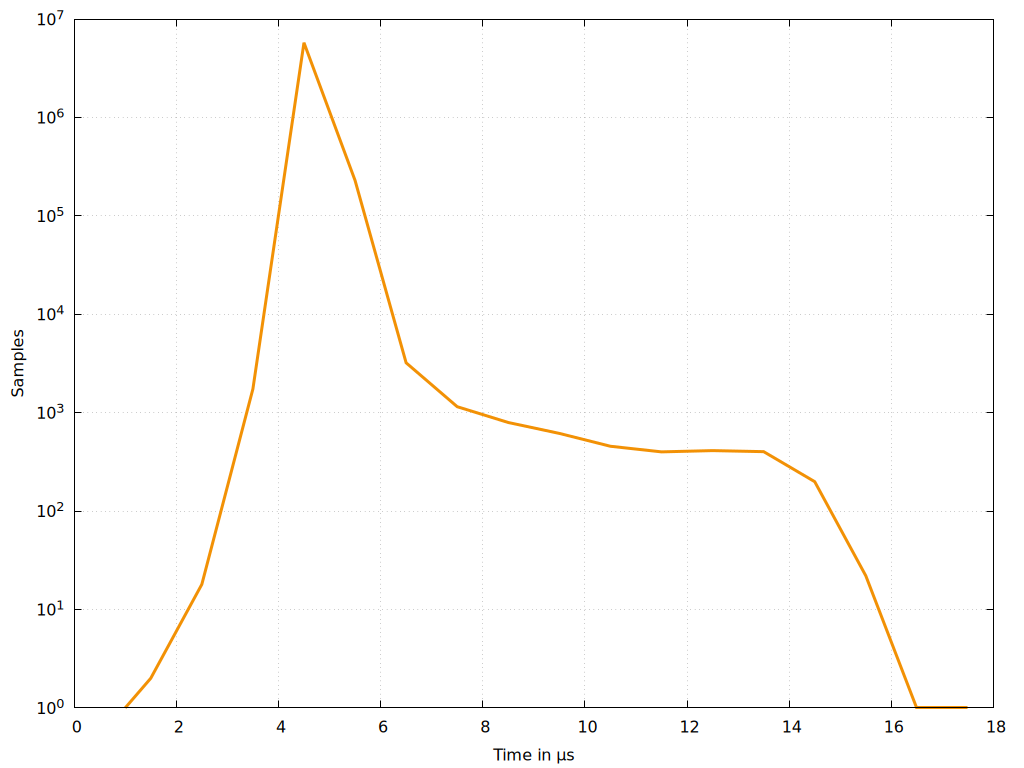
\includegraphics[width=0.7\columnwidth]{masterthesis-documentation/docs/sigmatek/xenomai/5rt_kernelparam_host/gnuplot_max_latency_rt_kernelparam_host.png}
	\caption[Latency Distribution of Salamander 4 after Host Configurations]{Latency Distribution of Salamander 4 Virtualization after tuning Host Configurations}
	\label{fig:max_latency_rt_kernelparam_host}
\end{figure}

\noindent The statistics obtained from this measurement are provided in Table~\ref{tab:latency_stats_virt_host} and Table~\ref{tab:latency_overrun_msw_new_virt_host}.

\begin{table}[H]
	\centering
	\caption{Latency Parameters for Host Configurations}
	\label{tab:latency_stats_virt_host}
	\begin{tabular}{|c|c|c|c|}
		\hline
		\textbf{Param} & \textbf{Samples} & \textbf{Average (µs)} & \textbf{Std Dev (µs)} \\ \hline
		\textbf{min}   & 599              & 2.998                 & 0.242                 \\ \hline
		\textbf{avg}   & 5,999,972        & 4.043                 & 0.255                 \\ \hline
		\textbf{max}   & 599              & 12.124                & 1.828                 \\ \hline
	\end{tabular}
\end{table}

\begin{table}[H]
	\centering
	\caption[Latency Statistics with Overrun Counts after Host Configurations]{Minimum, Average, and Maximum Latency with Overrun Counts after Host Configurations}
	\label{tab:latency_overrun_msw_new_virt_host}
	\begin{tabular}{|c|c|c|c|c|}
		\hline
		\textbf{Lat Min (µs)} & \textbf{Lat Avg (µs)} & \textbf{Lat Max (µs)} & \textbf{Overruns} \\ \hline
		2.591                 & 4.834                 & 18.441                & 0                 \\ \hline
	\end{tabular}
\end{table}

\noindent A worst latency value of 17.041\textmu s shows that the virtualized Salamander 4 OS got even more reliable with the host configurations.

\clearpage

\subsection{QEMU/KVM Configurations}\label{subsec:guest_configurations}
KVM allows the guest OS to run directly on the hardware, bypassing the need for traditional emulation which can introduce delays. QEMU, when used with KVM, provides hardware-assisted virtualization, which also lowers latency in the guest OS.

\subsubsection{Tune LAPIC Timer Advance}
The Local Advanced Programmable Interrupt Controller (LAPIC) is a built-in timer that handles the delivery of interrupts to the CPU.
It generates interrupts at a rate. This rate can be tuned in the \texttt{/sys/module/kvm/parameters/lapic\_timer\_advance\_ns} file to reduce the frequency of interrupts and therefore decrease the latency of the guest VM. The default value is ``-1'', which means that the kernel will automatically calculate an appropriate advance for the timer. Here, it is set to the value ``7500''. Hence, the timer interrupt will be delivered 7500 nanoseconds earlier than it is actually due. This gives the VM more time to handle it.

\subsubsection{Set QEMU Options for real-time VM}
QEMU provides several options that can be used to improve the real-time performance of the guest VM. Table~\ref{tab:qemu_options} briefly explains these options.

\begin{table}[H]
	\centering
	\caption{QEMU Options for Real-Time Performance}
	\label{tab:qemu_options}
	\setlength{\tabcolsep}{0.5em} % for the horizontal padding
	{\renewcommand{\arraystretch}{1.2}% for the vertical padding
		\begin{tabular}{|p{6.5cm}|p{8cm}|}
			\hline
			\textbf{QEMU Option}                                                             & \textbf{Description}                                                             \\\hline
			\texttt{-object memory-backend-ram,}\newline\texttt{id=ram0,size=4G,prealloc=on} & Locks the memory of the VM to 4GB and prevents it from being swapped out to disk \\\hline
			\texttt{-mem-prealloc} \newline \texttt{-mem-path /dev/hugepages/}               & Enables the use of hugepages and improves \newline memory access                 \\\hline
		\end{tabular}}
\end{table}

\noindent Code~\ref{script:qemu_def_tuned} shows the final QEMU script used to start the Salamander 4 virtualization, including these options.

\clearpage

\begin{lstlisting}[name={Tuned QEMU Script for starting Salamander 4 Virtualization},label={script:qemu_def_tuned}]
		#!/bin/sh

		if  [ ! -d drive-c/ ]; then
				echo "Filling drive-c/"
				mkdir drive-c/
				tar -C drive-c/ -xf stek-drive-c-image-sigmatek-core2.tar.gz
		fi
			
		exec taskset -c 4 chrt -f 99 qemu-system-x86_64 -M pc,accel=kvm -kernel ./bzImage \
		-m 2048 -drive file=salamander-image-sigmatek-core2.ext4,format=raw,media=disk \
		-append "console=ttyS0 console=tty1 root=/dev/sda rw panic=1 sigmatek_lrt.QEMU=1 ip=dhcp rootfstype=ext4 schedstats=enable nohlt idle=poll quiet xeno_hal.smi=1 xenomai.smi=1 threadirqs" \
		-net nic,model=e1000,netdev=e1000 -netdev bridge,id=e1000,br=nm-bridge \
		-fsdev local,security_model=none,id=fsdev0,path=drive-c -device virtio-9p-pci,id=fs0,fsdev=fsdev0,mount_tag=/mnt/drive-C \
		-device vhost-vsock-pci,guest-cid=3,id=vsock0 \
		-drive if=pflash,format=qcow2,file=ovmf.code.qcow2 \
		-object memory-backend-ram,id=ram0,size=4G,prealloc=on \
		-mem-prealloc -mem-path /dev/hugepages \
		-no-reboot -nographic
	\end{lstlisting}
\vspace{2em}
\noindent After QEMU configurations, the result of the \texttt{latency} test is depicted in Figure~\ref{fig:max_latency_rt_kernelparam_host_qemu}.

\begin{figure}[H]
	\centering
	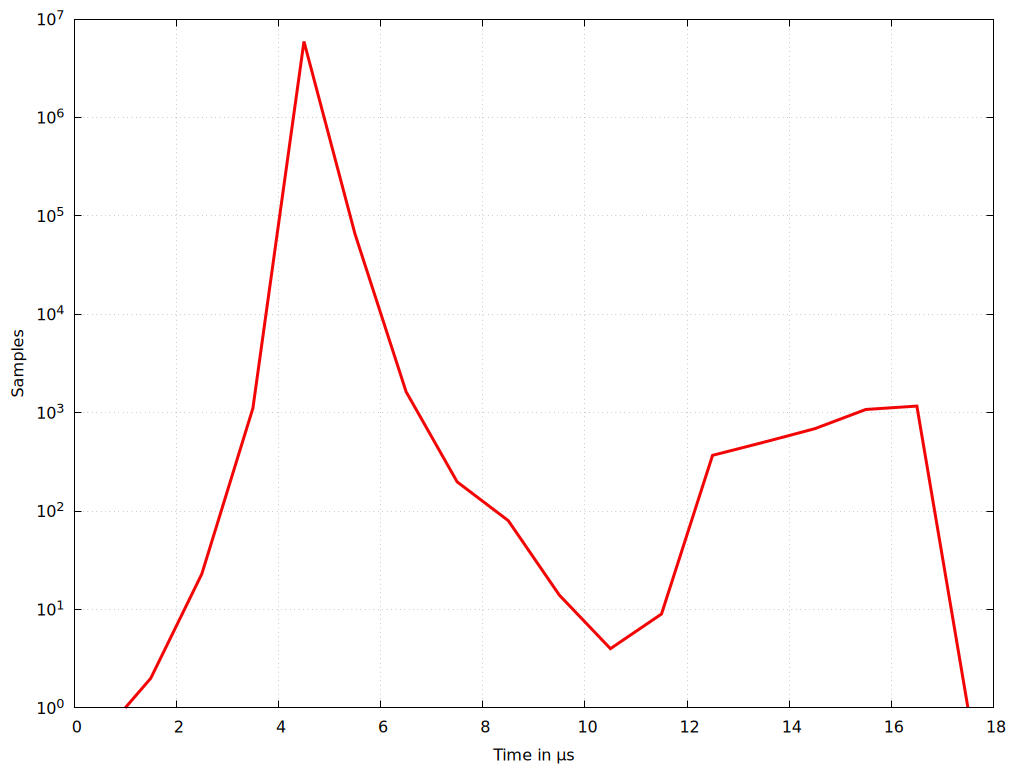
\includegraphics[width=0.7\columnwidth]{masterthesis-documentation/docs/sigmatek/xenomai/6rt_kernelparam_host_qemu/gnuplot_max_latency_rt_kernelparam_host_qemu.png}
	\caption[Latency Distribution of Salamander 4 after QEMU Configurations]{Latency Distribution of Salamander 4 Virtualization after tuning QEMU Configurations}
	\label{fig:max_latency_rt_kernelparam_host_qemu}
\end{figure}

\clearpage

\noindent The statistics obtained from this measurement are provided in Table~\ref{tab:latency_stats_virt_qemu} and Table~\ref{tab:latency_overrun_msw_new_virt_qemu}.

\begin{table}[H]
	\centering
	\caption{Latency Parameters after QEMU Configurations}
	\label{tab:latency_stats_virt_qemu}
	\begin{tabular}{|c|c|c|c|}
		\hline
		\textbf{Param} & \textbf{Samples} & \textbf{Average (µs)} & \textbf{Std Dev (µs)} \\ \hline
		\textbf{min}   & 599              & 3.125        & 0.432                 \\ \hline
		\textbf{avg}   & 5,999,973        & 4.018        & 0.291                 \\ \hline
		\textbf{max}   & 599              & 15.883       & 0.351                 \\ \hline
	\end{tabular}
\end{table}

\begin{table}[H]
	\centering
	\caption[Latency Statistics with Overrun Counts after QEMU Configurations]{Minimum, Average, and Maximum Latency with Overrun Counts after QEMU Configurations}
	\label{tab:latency_overrun_msw_new_virt_qemu}
	\begin{tabular}{|c|c|c|c|c|}
		\hline
		\textbf{Lat Min (µs)} & \textbf{Lat Avg (µs)} & \textbf{Lat Max (µs)} & \textbf{Overruns} \\ \hline
		2.614                 & 4.779                 & 17.134                & 0                 \\ \hline
	\end{tabular}
\end{table}

\noindent While the worst latency value did not change much, the standard deviation of the maximum latency samples of each second, with the test lasting 600 seconds and thus having 600 worst latencies, decreased. This means, the system is more stable and predictable, thanks to the real-time tunings that have been performed till this point.

\subsection{Guest OS Configurations}\label{subsec:guest_configurations}
The guest OS, Salamander 4, is already based on Xenomai and uses the Cobalt real-time core with the Dovetail extension. Therefore, no additional modifications were necessary for the guest OS itself. The focus was primarily on optimizing the host and virtualization layer to achieve the desired real-time performance.

\subsection{Other Configurations}
There are other configurations that may be relevant depending on the case. Linux Kernel Developer Steven Rostedt explains all relevant aspects of a real-time system that must be considered in~\cite{kernelrecipesKernelRecipes20162016} and gives insight for finding sources of latency on the Linux system in~\cite{thelinuxfoundationFindingSourcesLatency2020}. A Checklist for writing Linux real-time applications is provided by John Ogness in~\cite{thelinuxfoundationChecklistWritingLinux2020}. Every layer of the system stack must be deterministic to ensure predictable and reliable latency, including hardware, operating system, middleware and drivers, and the application software. ~\cite{HOWTOBuildRTapplication} and~\cite{RealtimeProgrammingLinux} describe the process of writing hard real time Linux programs using the real-time preemption patch in great detail. Various hardware and software tunings are listed in~\cite{KVMQemuVirtualization} and~\cite{RealTimePerformanceTuning2022}.

\clearpage

\section{Real-Time Robotic Application}\label{sec:robotic_application}
This chapter compares the latency of the Salamander 4 operating system before and after the real-time performance tunings with the latency of Salamander 4 running on bare metal. This comparison is done with the aid of a program that will be explained shortly. The goal is to understand how closely the performance of the virtualization can match that of the bare metal. The experimental setup includes a six-axis mini-robot, illustrated in Figure~\ref{fig:mini_robot}.

\begin{figure}[H]
	\centering
	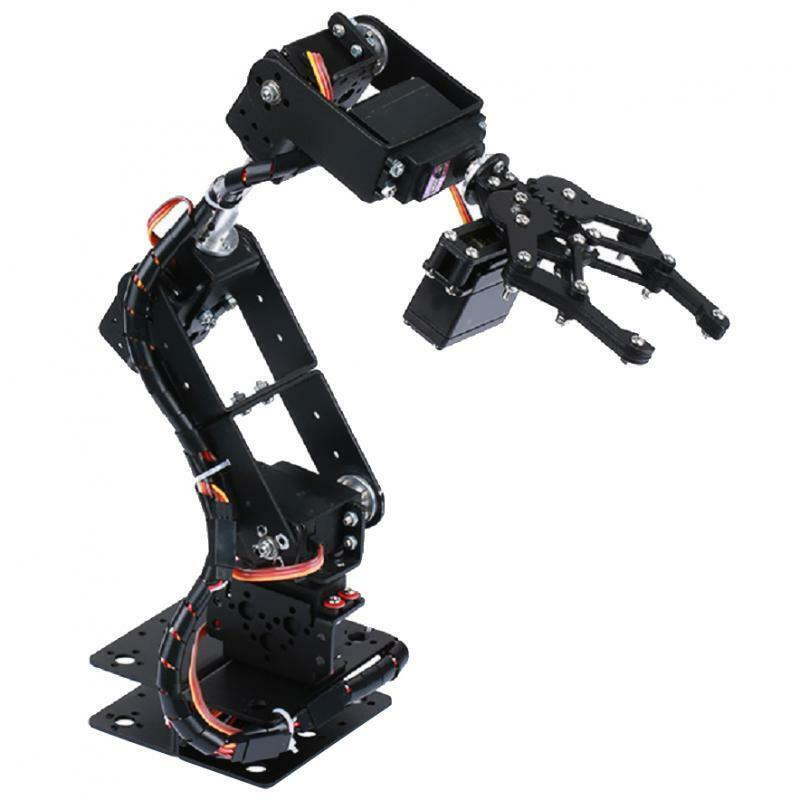
\includegraphics[width=0.3\columnwidth]{img/experiment/mini_robot.jpg}
	\caption[Mini-Robot of the Experiment]{Mini-Robot of the Experiment~\cite{6DFRoboticArm}}
	\label{fig:mini_robot}
\end{figure}

\noindent The robot arm consists of six MG996R digital servo motors~\cite{MG996RServoMotor}, equipped with a metal gearbox. The motor is able to rotate in a range of approximately 180 degrees and its position can be controlled with a high degree of accuracy. Each servo motor has three wires that need to be connected as shown in Figure~\ref{fig:servo}.

\begin{figure}[H]
	\centering
	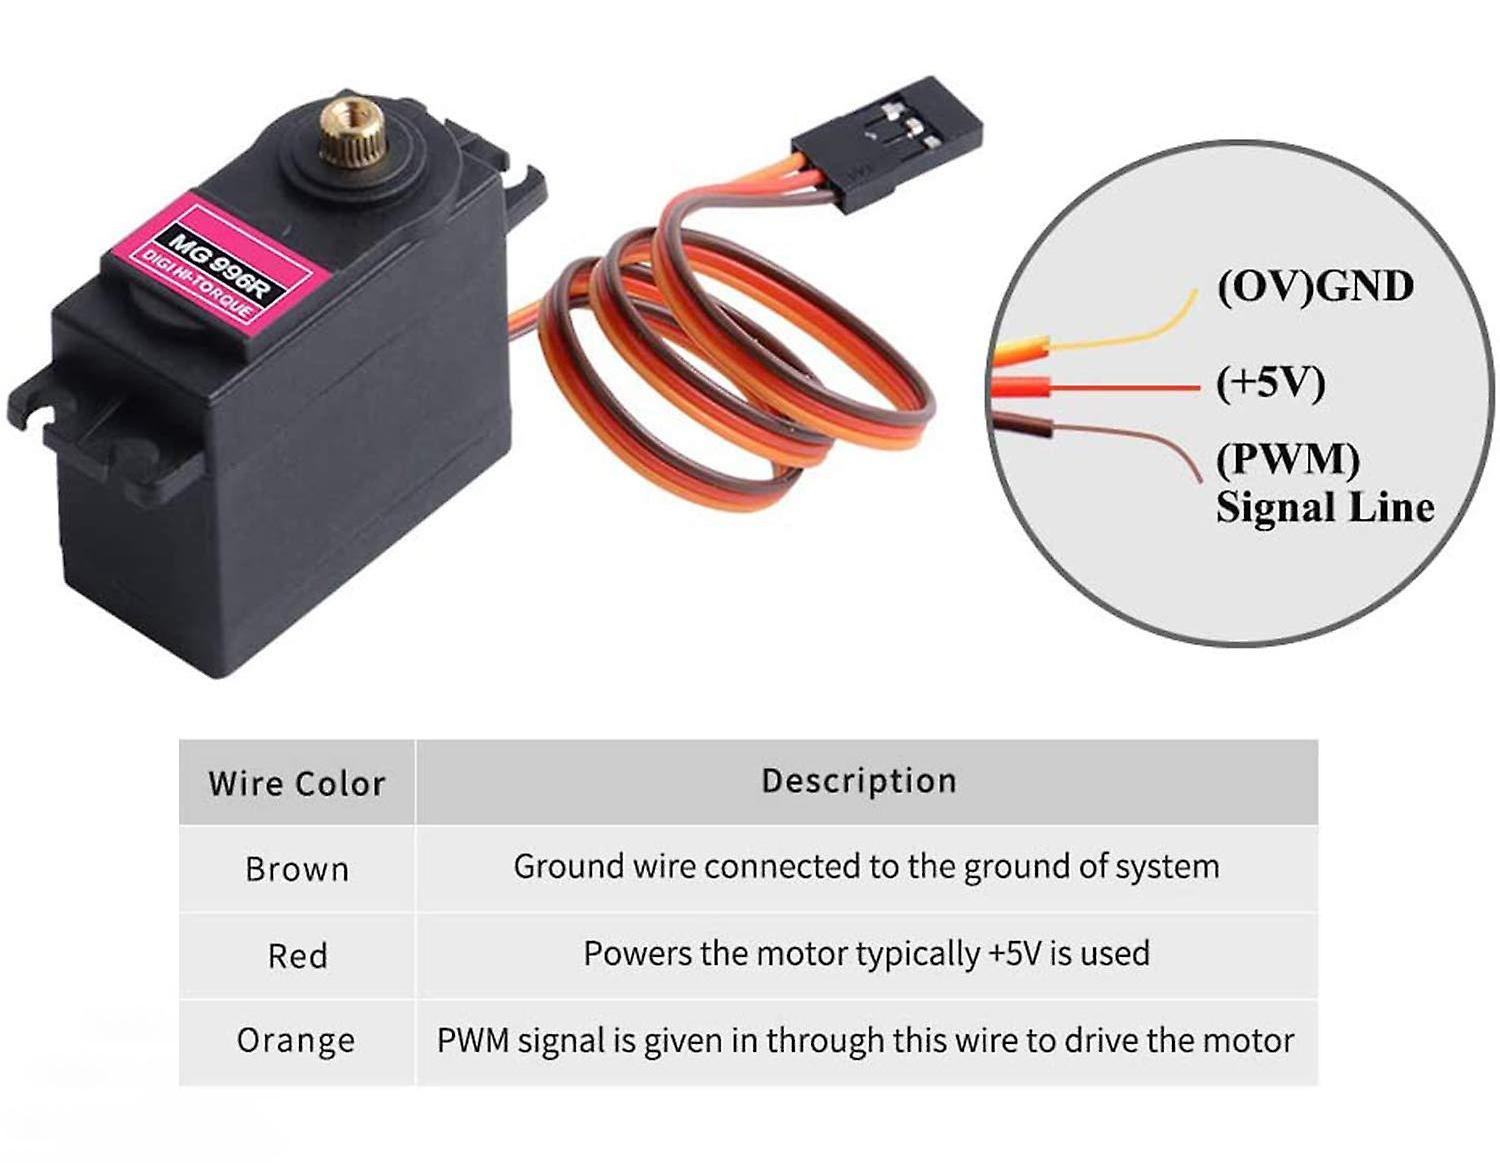
\includegraphics[width=0.7\columnwidth]{img/experiment/servo.jpg}
	\caption[MG996R Servo Motor]{MG996R Servo Motor~\cite{PackMg996rMetal}}
	\label{fig:servo}
\end{figure}

\noindent To drive the motor, it has to be powered using the red and brown wires and can be controlled by sending PWM signals to the orange wire. A 1,500 microsecond pulse every 20 milliseconds centers the servo. A 1,000 microsecond pulse turns it 90 degrees left, and a 2,000 microsecond pulse turns it 90 degrees right. This is depicted in Figure~\ref{fig:servo_angle}.

\begin{figure}[H]
	\centering
	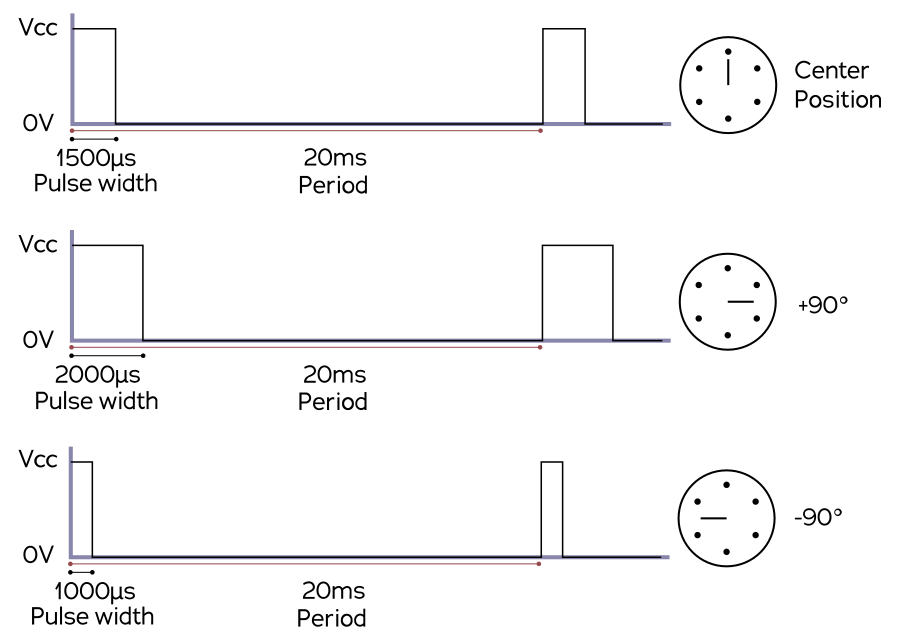
\includegraphics[width=0.7\columnwidth]{img/experiment/servo_angle.png}
	\caption[Controlling the MG996R Servo Motor]{Controlling the MG996R Servo Motor~\cite{twierengEmilyQuadrupedDog}}
	\label{fig:servo_angle}
\end{figure}

\noindent In this experiment, this PWM signal is generated by the proprietary PW 022 pulse width module of Sigmatek~\cite{DigitalOutputSIGMATEK}. Its connector layout is illustrated in Figure~\ref{fig:pw022_connectors}.

\begin{figure}[H]
	\centering
	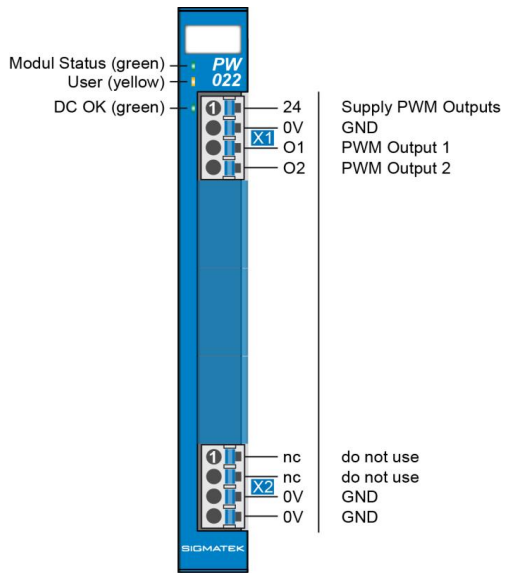
\includegraphics[width=0.5\columnwidth]{img/experiment/pw022_connectors.png}
	\caption[PW 022 Pulse Width Module Connector Layout]{PW 022 Pulse Width Module Connector Layout~\cite{DigitalOutputSIGMATEK}}
	\label{fig:pw022_connectors}
\end{figure}

\noindent The module has two +24 V switching PWM outputs with an adjustable frequency for controlling inductive loads. Since the mentioned servo motors operate between 4.8 volts and 7.2 volts~\cite{MG996RServoMotor}, this voltage needs to be reduced through resistors before supplying it to a servo motor. For this purpose, two resistors with resistances of 2500 kiloohms and 1000 kiloohms are connected in series. The voltage across each resistor is calculated using Ohm's law, which is given by equation~\ref{eq:ohms_law} below.
\begin{equation}
	\label{eq:ohms_law}
	V = I \cdot R
\end{equation}

\noindent In this equation, \(V\) represents the voltage across the resistor, \(I\) is the current flowing through the resistor, and \(R\) is the resistance of the resistor. The resulting voltages across the resistors are as follows:

\begin{itemize}
	\item The voltage across the 2.5 kiloohm resistor is approximately 17.14 volts.
	\item The voltage across the 1 kiloohm resistor is approximately 6.86 volts. This voltage is then supplied to the control wire of servo motor 1 of the mini-robot.
\end{itemize}

\noindent Connecting a second servo motor of the mini-robot means repeating the process of reducing the voltage through resistors for the second PWM output of the PW 022 module. The connection between the PW 022 module and the motor of the mini-robot is demonstrated in Figure~\ref{fig:pw022_minirobot_connection}.

\begin{figure}[H]
	\centering
	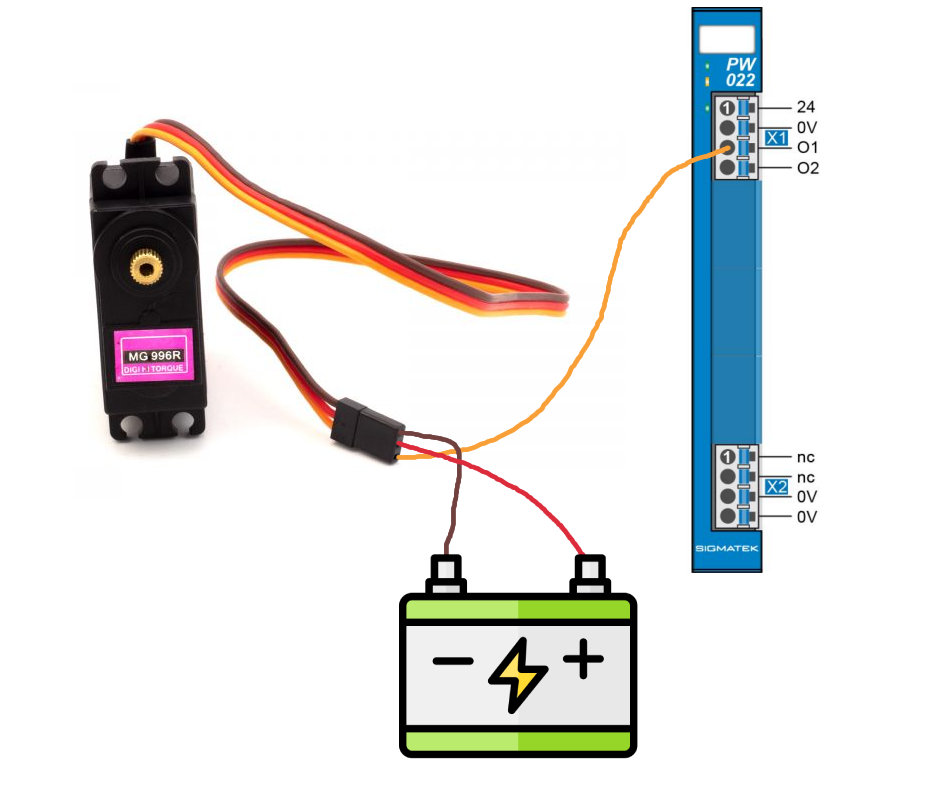
\includegraphics[width=0.7\columnwidth]{img/experiment/pw022_minirobot.png}
	\caption[Connection between PW 022 and Mini-Robot]{Connection between PW 022 and Mini-Robot~\cite{MG996RDigitalServo}}
	\label{fig:pw022_minirobot_connection}
\end{figure}

\noindent The program is written in Lasal Class 2 and is applied to all three mentioned versions of Salamander 4 to measure the reaction time of the robot to the commands. Prior to examining the software program, the next two subsections briefly explain the setup of each version of the experiment.

\subsection{Setup of Salamander 4 Bare Metal}
In this version, Salamander 4 runs on the CP 841~\cite{CPUUnitsSIGMATEK} CPU unit, specifically designed for the Salamander 4 operating system. The PW 022 modules are directly mounted on the CPU via the S-DIAS bus~\cite{SDIASSIGMATEK}. There are three PW 022 modules because each can control two motors simultaneously, and the mini-robot has six motors. The setup is visible on Figure~\ref{fig:hardware_tree}.

\begin{figure}[H]
	\centering
	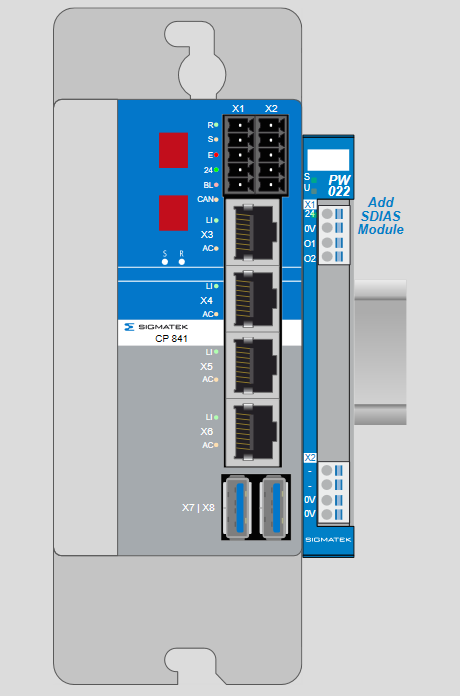
\includegraphics[width=0.45\columnwidth]{img/experiment/hardware_tree.png}
	\caption[Setup of Salamander 4 Bare Metal]{Setup of Salamander 4 Bare Metal}
	\label{fig:hardware_tree}
\end{figure}

\subsection{Setup of Salamander 4 Virtualization}\label{subsec:setup_experiment_virtualized}
In the virtualized setup of the experiment, the vCPU functionality of QEMU is used to connect QEMU with the PWM modules. In order to achieve that, the PCV 522 VARAN Manager PCI Insert Card~\cite{ControlsHMIsSIGMATEK}, which serves as a bridge between the PC and the rest of the setup, needs to be plugged into the PC. The command \texttt{lspci -nn} lists all PCI devices along with their vendor and device IDs. In this case, the command for binding the PCV 522 module to the VFIO-PCI driver was \texttt{sudo sh -c 'echo "5112 2200" > /sys/bus/pci/drivers/vfio-pci/new\_id'} with vendor ID \texttt{5112} and device ID \texttt{2200}.  To verify that the device has been successfully bound to the VFIO-PCI driver, \texttt{lspci -v} can be used. On top of the binding process, the QEMU script from the previous sections also needed to be modified to include the PCV 522 VARAN Manager PCI Insert Card in the virtualization. This is done by adding \texttt{-device\ vfio-pci,host=03:00.0 } to the QEMU script, where \texttt{03:00.0} refers to the PCI address of the device, with \texttt{03} being the bus number, \texttt{00} the device number, and \texttt{0} the function number. The final script can be seen in Code~\ref{script:qemu_def_pci}.

\clearpage

\vspace*{-5em}
\begin{lstlisting}[name={QEMU script for Salamander 4 Virtualization with PCI Configuration},label={script:qemu_def_pci}]
		#!/bin/sh

		if  [ ! -d drive-c/ ]; then
				echo "Filling drive-c/"
				mkdir drive-c/
				tar -C drive-c/ -xf stek-drive-c-image-sigmatek-core2.tar.gz
		fi
			
		exec taskset -c 4 chrt -f 99 qemu-system-x86_64 -M pc,accel=kvm -kernel ./bzImage \
		-m 2048 -drive file=salamander-image-sigmatek-core2.ext4,format=raw,media=disk \
		-append "console=ttyS0 console=tty1 root=/dev/sda rw panic=1 sigmatek_lrt.QEMU=1 ip=dhcp rootfstype=ext4 schedstats=enable nohlt idle=poll quiet xeno_hal.smi=1 xenomai.smi=1 threadirqs" \
		-net nic,model=e1000,netdev=e1000 -netdev bridge,id=e1000,br=nm-bridge \
		-fsdev local,security_model=none,id=fsdev0,path=drive-c -device virtio-9p-pci,id=fs0,fsdev=fsdev0,mount_tag=/mnt/drive-C \
		-device vhost-vsock-pci,guest-cid=3,id=vsock0 \
		-drive if=pflash,format=qcow2,file=ovmf.code.qcow2 \
		-object memory-backend-ram,id=ram0,size=4G,prealloc=on \
		-mem-prealloc -mem-path /dev/hugepages \
		-device vfio-pci,host=03:00.0 \
		-no-reboot -nographic
	\end{lstlisting}
\vspace{2em}
\noindent An additional Varan Connection module VI 021~\cite{InterfacesSplittersSIGMATEK} was required to enable the connection between the PCV 522 module and the PW 022 module that generates the signal to move the mini-robot. This setup is depicted in Figure~\ref{fig:virt_tree}.

\begin{figure}[H]
	\centering
	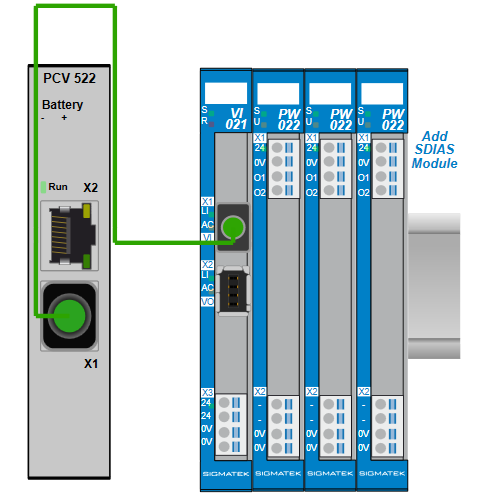
\includegraphics[width=0.5\columnwidth]{img/experiment/virt_tree.png}
	\caption[Setup of Salamander 4 Virtualization]{Setup of Salamander 4 Virtualization}
	\label{fig:virt_tree}
\end{figure}

\noindent Essentially, the CPU is being emulated by the vCPU functionality of QEMU, allowing the PCV 522 VARAN Manager PCI Insert Card and the Varan Connection module VI 021 to interact as if they were communicating with a physical CPU unit.

\subsection{Robotic Application}

Robots operate in real-time, meaning commands must be executed within a set time frame. As explained earlier, there are hard real-time systems, which must always meet their deadlines, and soft real-time systems, which can occasionally miss them. If a robot misses these deadlines, it can cause unwanted movements and jumpy behavior. The most crucial part of latency distribution for determinism are the outliers. Even if a system's latency is as expected 99\% of the time, the remaining 1\% can be worse than all the other measurements combined. Looking only at the mean and standard deviation misses these systemic issues.

\bigskip \noindent The impacts of real-time performance tunings on the determinism and latency of Salamander 4 virtualization were already shown in the previous chapter. In this chapter, these improvements are presented using a robotic application. This application is written in Lasal Class 2, as mentoned in Section~\ref{sec:application_context}. The program sequence is shown in Figure~\ref{fig:robotic_application_flow}.

\vspace{2em}

\begin{figure}[H]
	\centering
	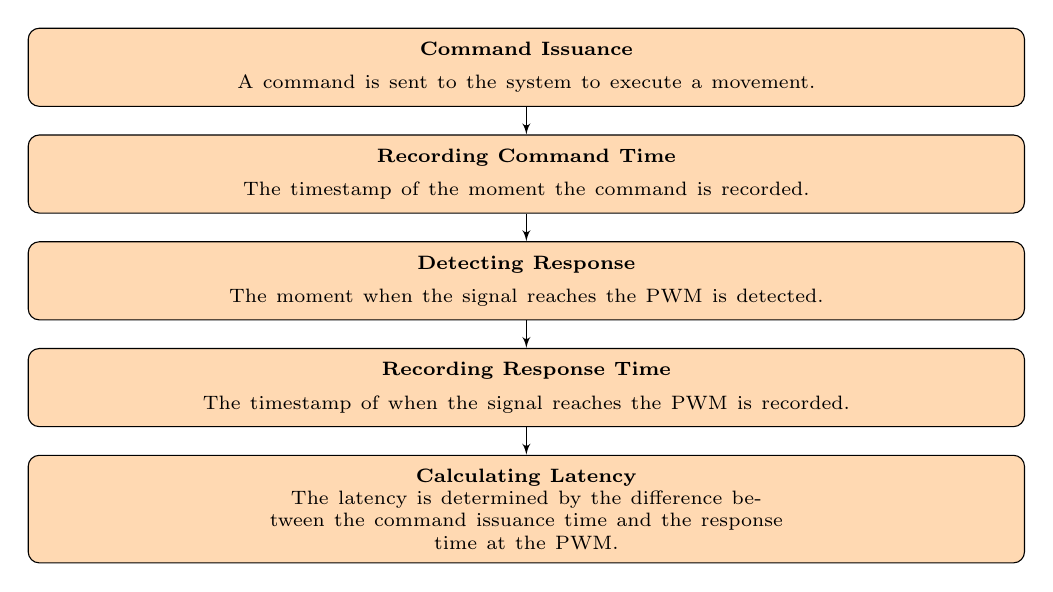
\begin{tikzpicture}[node distance = 0.35cm, auto, % Adjusted node distance
			block/.style={
					rectangle,
					draw,
					fill=orange!30,
					text width=35em,
					rounded corners,
					align=center,
					inner sep=0.5em % Adjusted inner separation
				},
			line/.style={draw, -latex'}
		]
		% Place nodes
		\node [block] (issue) {\scriptsize \textbf{Command Issuance}\\A command is sent to the system to execute a movement.};
		\node [block, below=of issue] (record1) {\scriptsize \textbf{Recording Command Time}\\The timestamp of the moment the command is recorded.};
		\node [block, below=of record1] (detect) {\scriptsize \textbf{Detecting Response}\\The moment when the signal reaches the PWM is detected.};
		\node [block, below=of detect] (record2) {\scriptsize \textbf{Recording Response Time}\\The timestamp of when the signal reaches the PWM is recorded.};
		\node [block, below=of record2] (calculate) {\scriptsize \textbf{Calculating Latency}\\The latency is determined by the difference between the command issuance time and the response \\\vspace{-0.5em} time at the PWM.};
		% Draw edges
		\path [line] (issue) -- (record1);
		\path [line] (record1) -- (detect);
		\path [line] (detect) -- (record2);
		\path [line] (record2) -- (calculate);
	\end{tikzpicture}
	\caption[Flowchart of Robotic Application]{Flowchart of Robotic Application}
	\label{fig:robotic_application_flow}
\end{figure}
\vspace{1em}

\noindent This latency measurement above is performed 1,000 times to get reliable results. These results are presented in the next subsubsections.



\begin{comment}
Ja, du denkst richtig! Wenn du die Latenz des Systems messen möchtest, die es benötigt, um das Signal bei der PWM anzukommen, und die 20 ms Signalperiode des Servomotors ignorieren möchtest, dann konzentrierst du dich auf die reine Reaktionszeit des Systems.

In diesem Fall misst du die Zeit von der Befehlsausgabe bis zum Eintreffen des Signals bei der PWM. Die 20 ms, die der Servomotor benötigt, um das Signal zu verarbeiten und die Bewegung zu starten, werden in deiner Latenzdefinition nicht berücksichtigt.

Das bedeutet, dass du die Latenz als die Zeit definierst, die das System benötigt, um das Signal an die PWM zu senden, ohne die zusätzliche Verzögerung durch die Signalperiode des Servomotors einzubeziehen.

	In diesem Versuch wird die Latenz des Systems gemessen, die benötigt wird, um das Signal von der Befehlsausgabe bis zum Eintreffen bei der PWM (Pulsweitenmodulation) zu erfassen. Die Signalperiode des Servomotors von 20 ms wird dabei ignoriert, da sie für die Definition der Systemlatenz nicht relevant ist. Die Latenz wird somit als die reine Reaktionszeit des Systems definiert, ohne die zusätzliche Verzögerung durch die Signalperiode des Servomotors zu berücksichtigen.
\end{comment}



\clearpage

\subsubsection{Latency in Salamander 4 Bare Metal}\label{subsubsec:latency_hardware}
\noindent The latency values for bare metal Salamander 4 OS aquired from the program above are demonstrated in Figure~\ref{fig:rtos_latencies} and detailed in Table~\ref{tab:robotic_application_latency_values_hardware}. 

\begin{figure}[H]
	\centering
	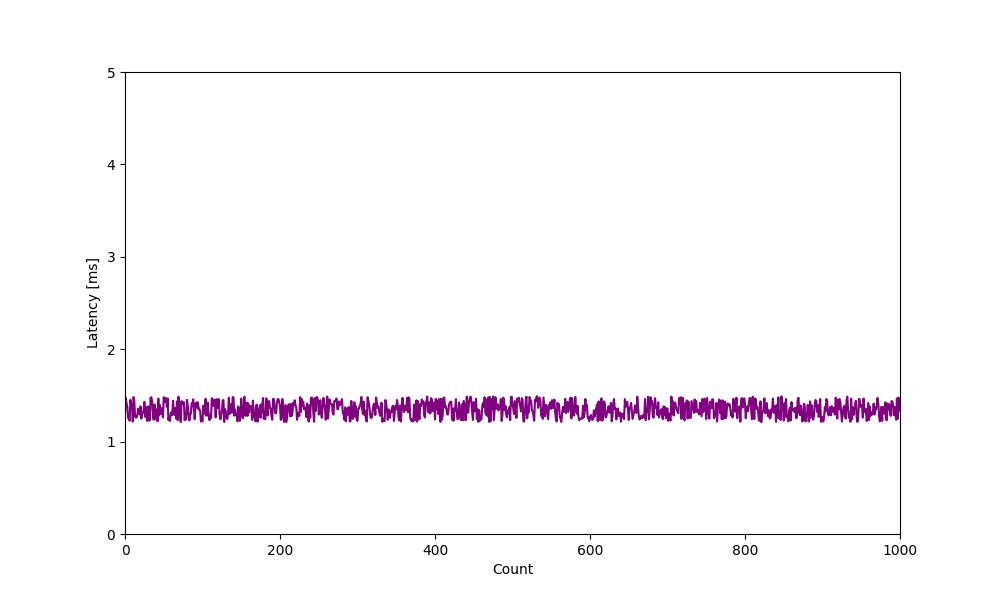
\includegraphics[width=1.0\columnwidth]{masterthesis-documentation/docs/resources/scripts/experiment/generated_latencies/rtos_latencies.png}
	\caption[Robotic Application Latency Values of Salamander 4 Hardware]{Robotic Application Latency Values of Salamander 4 Hardware}
	\label{fig:rtos_latencies}
\end{figure}

\begin{table}[H]
	\centering
	\caption{Robotic Application Latency Statistics Hardware}
	\label{tab:robotic_application_latency_values_hardware}
	\setlength{\tabcolsep}{0.5em} % for the horizontal padding
	{\renewcommand{\arraystretch}{1.2}% for the vertical padding
		\begin{tabular}{|l|l|l|l|l|}
			\hline
			\textbf{Samples} & \textbf{Lat Min (µs)} & \textbf{Lat Avg (µs)} & \textbf{Lat Max (µs)} & \textbf{Std Dev (µs)} \\ \hline

			1000             & 1.211                 & 1.347                  & 1.49                  & 0.082                   \\ \hline
		\end{tabular}}
\end{table}

\clearpage

\subsubsection{Latency in default Salamander 4 OS Virtualization}\label{subsubsec:latency_virtualization}
\noindent The latency values aquired for the default virtualization of Salamander 4 OS are demonstrated in Figure~\ref{fig:untuned_virt_latencies} and detailed in Table~\ref{tab:robotic_application_latency_values_virt_tun}. 

\begin{figure}[H]
	\centering
	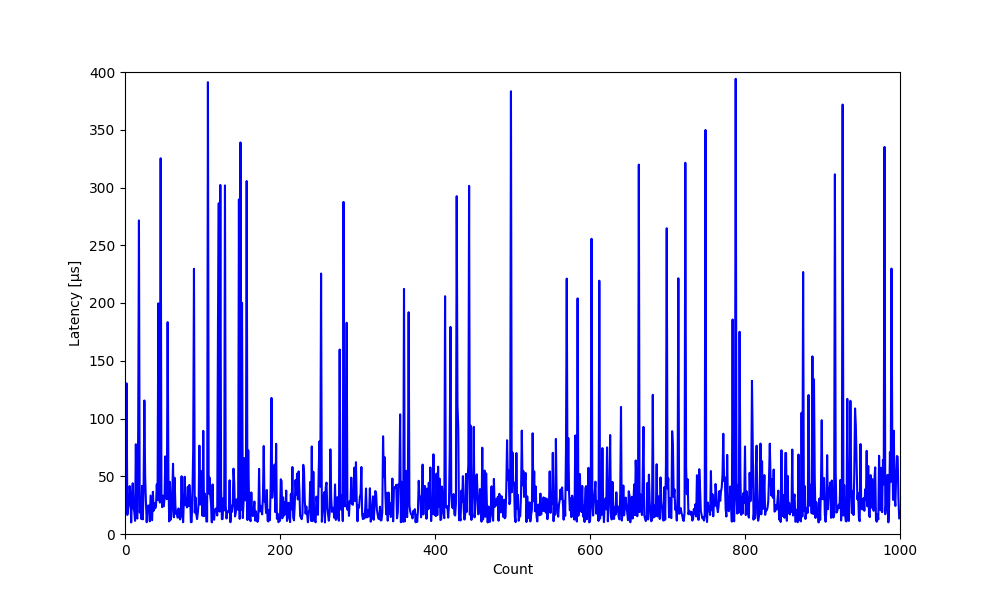
\includegraphics[width=1.0\columnwidth]{masterthesis-documentation/docs/resources/scripts/experiment/generated_latencies/untuned_virt_latencies.png}
	\caption[Robotic Application Latency Values of Salamander 4 Untuned Virtualization]{Robotic Application Latency Values of Salamander 4 Untuned Virtualization}
	\label{fig:untuned_virt_latencies}
\end{figure}

\begin{table}[H]
	\centering
	\caption{Robotic Application Latency Statistics Untuned Virtualization}
	\label{tab:robotic_application_latency_values_virt_def}
	\setlength{\tabcolsep}{0.5em} % for the horizontal padding
	{\renewcommand{\arraystretch}{1.2}% for the vertical padding
		\begin{tabular}{|l|l|l|l|l|}
			\hline
			\textbf{Samples} & \textbf{Lat Min (µs)} & \textbf{Lat Avg (µs)} & \textbf{Lat Max (µs)} & \textbf{Std Dev (µs)} \\ \hline
			1000             & 3.1                 & 24.603                  & 129.46            & 13.876                  \\ \hline
		\end{tabular}}
\end{table}

\clearpage

\subsubsection{Latency in tuned Salamander 4 OS Virtualization}\label{subsubsec:latency_virtualization}
\noindent The latency values aquired for the tuned virtualization of Salamander 4 OS are demonstrated in Figure~\ref{fig:tuned_virt_latencies} and detailed in Table~\ref{tab:robotic_application_latency_values_virt_tun}. 

\begin{figure}[H]
	\centering
	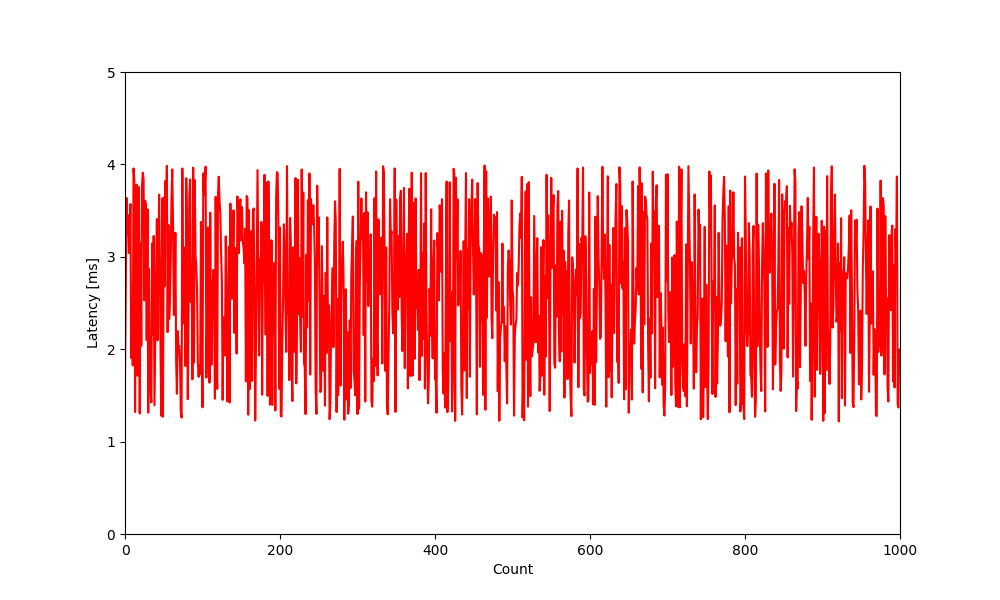
\includegraphics[width=1.0\columnwidth]{masterthesis-documentation/docs/resources/scripts/experiment/generated_latencies/tuned_virt_latencies.png}
	\caption[Robotic Application Latency Values of Salamander 4 Tuned Virtualization]{Robotic Application Latency Values of Salamander 4 Tuned Virtualization}
	\label{fig:tuned_virt_latencies}
\end{figure}
\begin{table}[H]
	\centering
	\caption{Robotic Application Latency Statistics Tuned Virtualization}
	\label{tab:robotic_application_latency_values_virt_tun}
	\setlength{\tabcolsep}{0.5em} % for the horizontal padding
	{\renewcommand{\arraystretch}{1.2}% for the vertical padding
		\begin{tabular}{|l|l|l|l|l|}
			\hline
			\textbf{Samples} & \textbf{Lat Min (µs)} & \textbf{Lat Avg (µs)} & \textbf{Lat Max (µs)} & \textbf{Std Dev (µs)} \\ \hline
			1000             & 1.219                 & 2.62                  & 3.988            & 0.182                   \\ \hline
		\end{tabular}}
\end{table}

\clearpage

\begin{comment}

\chapter{To Include}\label{cha:to_include}

\section{KVM Entry and KVM Exit}\label{subsubsec:kvm_entry_exit}
\textcolor{red}{\noindent Upon isolating a CPU to the QEMU process, it was anticipated that the guest would utilize nearly 100\% of the CPU's capacity, with minimal to no intervention from the host. However, the isolcpus function only isolates CPUs from the scheduler, meaning that user-space processes won't be scheduled on these CPUs, but kernel tasks and interrupts can still utilize the CPU.This led to the investigation of the causes for the observed high and inconsistent latency. The guest operates within the~\texttt{kvm\_entry} and~\texttt{kvm\_exit} events of the host. Kernelshark revealed a high frequency of~\texttt{kvm\_exit} events, indicating that the guest frequently relinquishes control of the CPU back to the host. This frequent switching hinders the guest's ability to run continuously, thereby increasing the virtualization latency.}

\textcolor{red}{To further understand this, trace-cmd was employed to trace various events in the host-guest communication, including the reasons for these events. Specifically, the causes for~\texttt{kvm\_exit} events were analyzed. The command sudo trace-cmd record -e all -A @3:823 --name Salamander4 -e all was executed on the host for a duration of 5 seconds. The results in Figure~\ref{fig:kvm_exit_taskset} were obtained. Additionally, Table~\ref{tab:kvm_exit} provides a short description of the observed~\texttt{kvm\_exit} events.}

\vspace{2em}
\begin{table}[H]
	\centering
	\begin{tabular}{|l|p{0.62\textwidth}|}
		\hline
		\textbf{Exit Reason} & \textbf{Description}                                     \\ \hline
		APIC\_WRITE          & Triggered when the guest writes to its APIC.             \\ \hline
		EXTERNAL\_INTERRUPT  & Triggered by external hardware interrupts.               \\ \hline
		HLT                  & Triggered when the guest executes the HLT instruction.   \\ \hline
		EPT\_MISCONFIG       & Triggered by a misconfiguration in the EPT.              \\ \hline
		PREEMPTION\_TIMER    & Triggered when the host's preemption timer expires.      \\ \hline
		PAUSE\_INSTRUCTION   & Triggered when the PAUSE instruction is executed.        \\ \hline
		EPT\_VIOLATION       & Triggered by a violation of the EPT permission settings. \\ \hline
		IO\_INSTRUCTION      & Triggered when the guest executes an I/O instruction.    \\ \hline
		EOI\_INDUCED         & Triggered when an EOI signal is sent to the APIC.        \\ \hline
		MSR\_READ            & Triggered when the guest reads from a MSR.               \\ \hline
		CPUID                & Triggered when the guest executes the CPUID instruction. \\ \hline
	\end{tabular}
	\caption{Description of kvm\_exit reasons}
	\label{tab:kvm_exit}
\end{table}

\textcolor{red}{\noindent In the process of analyzing the~\texttt{kvm\_exit} events, several reasons for these exits were identified. The most frequent among these were the~\texttt{APIC\_WRITE} and~\texttt{HLT} events. The former is initiated when the guest writes to its Advanced Programmable Interrupt Controller (APIC), a component of the CPU that manages hardware interrupts. The latter occurs when the guest executes the HLT instruction, effectively halting the CPU until the next external interrupt is fired. Other significant but less frequent events included~\texttt{EXTERNAL\_INTERRUPT} and~\texttt{IO\_INSTRUCTION}. These events are indicative of the guest's interaction with hardware devices and its execution of I/O operations. Events such as~\texttt{EPT\_MISCONFIG} and~\texttt{PREEMPTION\_TIMER} were also noted. These could potentially signal issues with memory management and the host's scheduling of the guest. While events like~\texttt{PAUSE\_INSTRUCTION},~\texttt{EPT\_VIOLATION},~\texttt{EOI\_INDUCED},~\texttt{MSR\_READ}, and~\texttt{CPUID} were the least frequent, they still provide valuable insights into the guest's behavior and the host-guest interaction.}

\textcolor{red}{\noindent When the script is started from the host, the QEMU process can be scheduled to run on any available core, as it is not bound to a specific CPU core. This means that the QEMU process may frequently switch between different cores, leading to an increase in latency. As the goal was to reduce latency in the guest, the first step was to isolate a CPU of the host and dedicate it solely to the QEMU process, so that it cannot be used for other tasks on the user level. Without CPU isolation, context switches take place at the operating system level and not at the hypervisor level. This explains why there are fewer~\texttt{kvm\_exit} events. However, this will also, as previously shown, lead to higher latency, as context switches at the operating system level generally take longer than a~\texttt{kvm\_exit} and ~\texttt{kvm\_entry}. When the CPU was dedicated to the QEMU process, on the other hand, there was a significant increase in~\texttt{kvm\_exit} events. This is because every context switch takes place at the hypervisor level. Nevertheless, lower latency was achieved thereby, as the qemu process is no longer influenced by the CPU scheduling of the operating system.}

``korrekt''

\noindent \enquote{This LaTeX.}

\section{Trace-cmd and Kernelshark}
After analyzing the inital latency of both versions, Trace-cmd and Kernelshark were used to further inspect the reasons that caused this divergence.

\section{Host and Guest tasks}
\vspace{2em}
\begin{table}[H]
\centering
\begin{minipage}{.5\textwidth}
\centering
\caption{Host report CPU19 (Total of 445.908)}
\label{tab:results_host_report}
\begin{tabular}{|c|c|c|}
	\hline
	PID    & Task                          & Count   \\ \hline
	182579 & qemu-system-x86               & 302.748 \\ \hline
	0      & \textless{}idle\textgreater{} & 112.911 \\ \hline
	182618 & vhost                         & 21.204  \\ \hline
	182572 & qemu-system-x86               & 7.597   \\ \hline
	182755 & qemu-system-x86               & 644     \\ \hline
	182754 & qemu-system-x86               & 643     \\ \hline
	181870 & kworker/19:1                  & 139     \\ \hline
	3820   & kworker/19:1H                 & 16      \\ \hline
	94     & migration/19                  & 6       \\ \hline
\end{tabular}
%
\begin{minipage}{.5\textwidth}
\centering
\caption{Guest report (Total of 362.370)}
\label{tab:results_guest_report}
\begin{tabular}{|c|c|c|}
	\hline
	PID & Task                          & Count   \\ \hline
	0   & \textless{}idle\textgreater{} & 150.744 \\ \hline
	331 & LRT-Main                      & 56.697  \\ \hline
	377 & trace-cmd                     & 48.507  \\ \hline
	346 & CLI                           & 26.426  \\ \hline
	378 & kthreadd                      & 25.837  \\ \hline
	340 & MainTaskLow                   & 19.291  \\ \hline
	339 & \textless{}...\textgreater{}  & 9.980   \\ \hline
	34  & MainTaskHigh                  & 9.185   \\ \hline
	327 & LE-Logger                     & 4.965   \\ \hline
	369 & kworker/0:0                   & 2.793   \\ \hline
	321 & kWorker-LRT                   & 2.542   \\ \hline
	328 & LRTMgr-Main                   & 1.651   \\ \hline
	34  & LrtMgrCyclic                  & 1.220   \\ \hline
	332 & cobalt\_printf                & 1.112   \\ \hline
	325 & LE-System                     & 534     \\ \hline
	343 & TCP-Listen                    & 187     \\ \hline
	15  & rcu\_preempt                  & 162     \\ \hline
	25  & kcompactd0                    & 122     \\ \hline
	58  & kworker/0:1H                  & 96      \\ \hline
	63  & kworker/u2:2                  & 89      \\ \hline
	8   & jbd2/sda-8                    & 86      \\ \hline
	22  & kworker/0:1                   & 56      \\ \hline
	1   & init                          & 31      \\ \hline
	2   & kthreadd                      & 25      \\ \hline
	375 & trace-cmd                     & 24      \\ \hline
	14  & ksoftirqd/0                   & 8       \\ \hline
\end{tabular}

\end{table}

\noindent In the following, the host and guest tasks along with their impact on system latency are briefly described.

\begin{itemize}
	\item \textbf{qemu-system-x86}: Part of the QEMU process and specifically, this task emulates x86 systems. In Table~\ref{tab:results_host_report}, it occurs four times under different PIDs, hence there are four threads of it.
	\item \textbf{<idle>}: This represents the idle time of the CPU, hence it is not being used by any process, allowing to save power. The system halts until the next interrupt, which could be a timer interrupt, I/O interrupt, etc.
	\item \textbf{vhost}: A kernel module which improves virtual input/output (virtio) performance by handling virtqueues in the kernel, thereby reducing context switches and system calls.
	\item \textbf{kworker/19:1}: A kernel worker thread created by the Linux kernel, kworker/19:1 performs work in response to system events. The number after the slash and colon indicate the CPU core and internal ID of the worker thread, respectively.
	\item \textbf{kworker/19:1H}: Similar to kworker/19:1, kworker/19:1H is a kernel worker thread, with the ‘H’ suggesting that this thread handles hardware interrupts.
	\item \textbf{migration/19}: The migration process is a kernel process that balances load across CPU cores by moving threads from one CPU to another. The number after the slash indicates the CPU core to which the migration process is bound. (URL: \url{https://elixir.bootlin.com/linux/latest/source/kernel/sched/core.c#L2325})

\end{itemize}

The Figure below (deleted) compares non-optimized guest latency with optimized guest latency and includes optimized bare metal latency as a reference. The data shows that a 40\% reduction in QD1 latency is achievable through system tuning.

\end{comment}

\chapter{Results}\label{cha:results}
The goal was to virtualize the Salamander 4 OS and bring its real-time performance closer to that of the hardware version and guarantee deterministic and reliable behavior. This chapter summarizes the results after the real-time performance tunings, both in terms of the \texttt{latency} program and the robotic application. Figure~\ref{fig:max_latency_combined_results} displays the change in latency after each real-time performance tuning, detailed in Section~\ref{sec:real-time_tunings}. 

\begin{figure}[H]
	\centering
	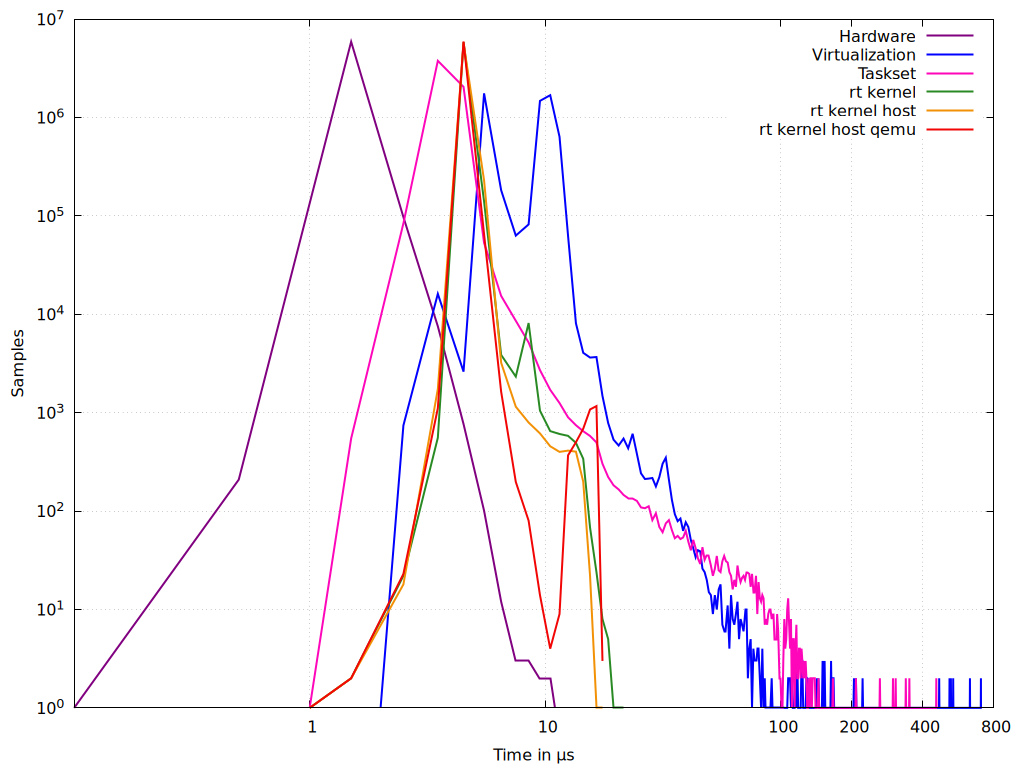
\includegraphics[width=0.70\columnwidth]{masterthesis-documentation/docs/sigmatek/xenomai/012456combined/gnuplot_combined_max_latency.png}
	\caption[Comparison of Latency Distribution of Salamander 4 Configurations]{Comparison of Latency Distribution of Salamander 4 under different Configurations}
	\label{fig:max_latency_combined_results}
\end{figure}

\noindent As mentioned earlier in Section~\ref{sec:approach}, these modifications were added sequentially and tested together. Previous tunings were not reverted when moving to the next tunings. Table~\ref{tab:latency_tables_combined} gives an overview of the most important metrics of the measurements after each tuning. 

\begin{table}[H]
	\centering
	\footnotesize
	\caption{Comparison of Latency Statistics in Salamander 4 under different Configurations}
	\label{tab:latency_tables_combined}
	\begin{tabular}{|c|c|c|c|c|c|}
		\hline
		\textbf{Tuning} & \textbf{Lat Min (µs)} & \textbf{Lat Avg (µs)} & \textbf{Lat Max (µs)} & \textbf{Overruns} \\ \hline
		Salamander 4 BM        & 0.613                 & 1.380                 & 10.709            & 0                 \\ \hline
		Unt. Salamander 4 V.        & 2.536                 & 8.940                 & 707.622      & 43                \\ \hline
		After BIOS Conf.   & 0.969                 & 3.948                 & 457.545               & 94                \\ \hline
		After Kernel Conf. & 2.545                 & 4.811                 & 21.694                & 0                 \\ \hline
		After Host Conf.   & 2.591                 & 4.834                 & 18.441                & 0                 \\ \hline
		After QEMU Conf.   & 2.614                 & 4.779                 & 17.134                & 0                 \\ \hline
	\end{tabular}
\end{table}

\clearpage 

\noindent The improved latency was also tested with the robotic application in Subsection~\ref{sec:robotic_application}. The difference between the command time and the time the signal reaches the PWM was measured 1,000 times for the untuned, tuned and hardware version of Salamander 4. The results are visualized in Figure~\ref{fig:combined_latencies}. 

\begin{figure}[H]
	\centering
	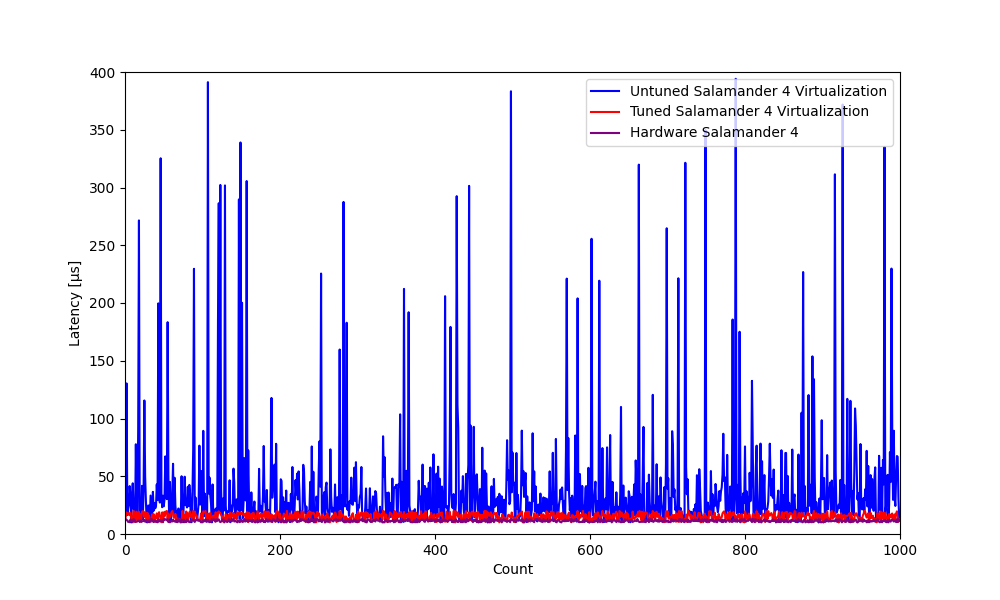
\includegraphics[width=1.0\columnwidth]{masterthesis-documentation/docs/resources/scripts/experiment/generated_latencies/combined_latencies.png}
	\caption[Comparison of Robotic Application Latency of Salamander 4 Configurations]{Comparison of Robotic Application Latency of Salamander 4 under different Configurations}
	\label{fig:combined_latencies}
\end{figure}

\noindent This response latency measurement above was performed 1,000 times to get reliable results. These results are presented in Table~\ref{tab:robotic_application_latency_values_combined}.

\begin{table}[H]
	\small
	\centering
	\caption{Comparison of Robotic Application Latency Statistics}
	\label{tab:robotic_application_latency_values_combined}
	\setlength{\tabcolsep}{0.5em} % for the horizontal padding
	{\renewcommand{\arraystretch}{1.2}% for the vertical padding
		\begin{tabular}{|l|l|l|l|l|l|}
			\hline
			\textbf{Tuning} & \textbf{Samples} & \textbf{Lat Min (ms)} & \textbf{Lat Avg (ms)} & \textbf{Lat Max (ms)} & \textbf{Std Dev (ms)} \\ \hline
			Hardware & 1000 & 1.211 & 1.347 & 1.49 & 0.082 \\ \hline
			Untuned Virtualization & 1000 & 3.1 & 24.603 & 129.46 & 13.876 \\ \hline
			Tuned Virtualization & 1000 & 1.219 & 2.62 & 3.988 & 0.812 \\ \hline
		\end{tabular}}
\end{table}

\clearpage

\chapter{Discussion}\label{cha:discussion}
This master's thesis shows that the real-time performance tunings applied to the virtualized Salamander 4 OS have a positive impact on reducing latency and improving determinism. The maximum latency in the final tuned version of Salamander 4 Virtualization is significantly lower than in the default setup. The worst latency value in a 10 minute measurement span decreased from 707.622\textmu s to 17.134\textmu s after tuning  BIOS, kernel, host, guest and QEMU/KVM configurations. Especially the BIOS and kernel configurations played a crucial role in reducing the maximum latency, with a major fall to 21.694\textmu s. From this moment on, there were also no overruns in the test any longer. The host configurations, including the PREEMPT-RT patch, CPU and interrupt affinity, and real-time prioritization of QEMU further reduced latency a little bit down to 18.441\textmu s. The guest OS, Salamander 4, already had real-time capabilities through Xenomai. The focus was primarily on optimizing the host and virtualization layer to achieve the desired real-time performance. Finally, QEMU/KVM configurations, such as tuning the LAPIC timer advance and using hugepages brought the latency down a little more to the final worst latency value of 17.134\textmu s in 10 minutes. This value is very close to the bare metal value of 10.709\textmu s. The goal was set to achieving latency values below 50 microseconds in the duration of the measuremenet. This goal is acheived.

\bigskip \noindent As a next step, the robotic application in a practical scenario also demonstrates and validates the improvement of the tuned virtualization compared to the unmodified virtualization. The difference between the command time and the time the signal reaches the PWM was measured 1,000 times for the untuned, tuned, and hardware version of Salamander 4. The most important metric here is also the worst latency of the signal reaching the PWM. It dropped from 129 ms to 3.988 ms in the developed application. Comparing this to the worst latency value of the hardware version, which is 1.49 ms, it is apparent that the tuned virtualization through real-time performance configurations came very close to the determinism and reliability of the hardware.

\bigskip \noindent It is important to underline one more time the fact that these modifications were added sequentially and tested together. First, the BIOS was configured, followed by the kernel. The BIOS settings were not reverted when moving to the kernel configurations. Next, the host was configured, but the BIOS and kernel settings remained unchanged. The guest configurations were not changed since Xenomai already provides real-time capabilities. Finally, QEMU/KVM settings were applied. This means that the configurations are not isolated but are applied and then tested as a whole.

\clearpage

\chapter{Summary and Outlook}\label{cha:summary_and_outlook}


Hardware-based systems are limited in adaptability and can be costly, especially when scaling operations. Physical access for updates and maintenance is challenging, leading to downtime and lost productivity. While virtualization addresses these issues, it introduces increased overhead and latency.

\bigskip \noindent In this master's thesis, the goal was the virtualization of a real-time operating system to control a robot, with a focus on compliance with real-time determinism. Specifically, the aim was to bring the latency of the virtualized Salamander 4 closer to that of the bare metal version, thereby providing a comprehensive blueprint for making a virtualized guest system in a host system real-time capable with deterministic behavior. Salamander 4 is built with Yocto, employs hard real-time with Xenomai 3 and is virtualized through QEMU/KVM. The testing robot was connected to the OS via a VARAN bus interface.

\bigskip \noindent The initial latency values were first measured with the \texttt{latency} program of the Xenomai tool suite. The tests were conducted with a sampling period of 100 µs, using a periodic user-mode task, and was assigned a priority of 99. If any sample's latency value was greater than 100µs, this was considered an overrun. There was a significant initial gap in latency statistics between the virtualized Salamander 4 and the Salamander 4 on bare metal. To address this gap, an extensive tuning process was carried out to achieve real-time performance and determinism. These modifications were added sequentially and tested together. First, the BIOS was configured, followed by the kernel. The BIOS settings were not reverted when moving to the kernel configurations. After these two steps, the worst latency decreased from an initial value of 707.62~\textmu s to 21.694\textmu s.  From this moment on, there were also no overruns in the test any longer. The host configurations, including the PREEMPT-RT patch, CPU and interrupt affinity, and real-time prioritization of QEMU further reduced latency a little bit down to 18.441\textmu s. The guest OS, Salamander 4, already had real-time capabilities through Xenomai. The focus was primarily on optimizing the host and virtualization layer to achieve the desired real-time performance. Finally, QEMU/KVM configurations, such as tuning the LAPIC timer advance and using hugepages brought the latency down a little more to the final worst latency value of 17.134\textmu s in 10 minutes. This value is very close to the bare metal value of 10.709\textmu s. The goal was set to achieving latency values below 50 microseconds in the duration of the measuremenet. This goal was acheived.

\bigskip \noindent On top of that, a robotic application further confirmed the improvements. The difference between the command time and the time the signal reaches the PWM was measured 1,000 times for the untuned, tuned and hardware version of Salamander 4. The worst latency of the signal reaching the PWM dropped from an inital value of 129ms to 3.988ms. Comparing this to the worst latency value of the hardware version, which was 1.49ms, it is apparent that the tuned virtualization through real-time performance configurations came very close to the determinism and reliability of the hardware.

\bigskip \noindent While this thesis provides a comprehensive blueprint for making a virtualized guest system in a host system real-time capable with deterministic behavior, future work can be done to extend this knowledge. Additional configurations and optimizations of the virtualization layer can be done and tested to further reduce latency and improve determinism. Other than that, the use of other hypervisors and virtualization technologies can be investigated to compare their performance for real-time applications. Moreover, extensive testing of the virtualized system under various workloads can be conducted to evaluate its performance and reliability in different conditions and stressed situations, as demonstrated by \citeauthor{huang2015performance}~\cite{huang2015performance}, \citeauthor{kirovaImpactModernVirtualization2019}~\cite{kirovaImpactModernVirtualization2019} or \citeauthor{adamPerformanceAssessmentLinux2021}~\cite{adamPerformanceAssessmentLinux2021}.

\begin{comment}
~\cite{canbazPerformanceAnalysisRealtime2022}
~\cite{WhatRealtimeLinux}
~\cite{malallahComprehensiveStudyKernel2021}
~\cite{wangRealtimeEmbeddedSystems2017}
~\cite{buttazzoHardRealtimeComputing2024}
~\cite{lipariRealTimeSchedulingHard2015}
~\cite{amarpreetHardRealTime2009}
~\cite{queirozTestingLimitsGeneralpurpose2023}
~\cite{pixelartSIGMATEKKompletteAutomatisierungssysteme}
~\cite{WelcomeYoctoProject}
~\cite{XenomaiXenomai}
~\cite{perneelRealtimeCapabilitiesStandard2015}
~\cite{reghenzaniRealTimeLinuxKernel2020}
~\cite{adamRealTimePerformanceResponse2021}
~\cite{cinqueVirtualizingMixedCriticalitySystems2022}
~\cite{sandstromVirtualizationTechnologiesEmbedded2013}
~\cite{taccariEmbeddedRealTimeVirtualization2014}
~\cite{javierperezHowRealTime2022}
~\cite{guStateoftheArtSurveyRealTime2012}
~\cite{garcia-vallsChallengesRealtimeVirtualization2014}
~\cite{scordinoRealTimeVirtualizationIndustrial2020}
~\cite{maPerformanceTuningKVMbased2013}
~\cite{junzhangPerformanceAnalysisKVMBased2010}
~\cite{broskyShieldedProcessorsGuaranteeing2003}
~\cite{RealTimePerformanceTuning2022}
~\cite{yoonRealTimePerformanceAnalysis2009}
~\cite{kiszkaLinuxRealTimeHypervisor2009}
~\cite{mckenneyRealTimeVs2008}
~\cite{deoliveiraDemystifyingRealTimeLinux2020}
~\cite{gabrielResourceAwareParameterTuning2019}
~\cite{bhardwajVirtualizationCloudComputing2021}
~\cite{abbasiExploringOpenStackScalable2023}
~\cite{mahfoudRealTimePredictiveMaintenanceBased2024}
~\cite{queirozContainerbasedVirtualizationRealtime2024}
~\cite{cinqueEvaluatingVirtualizationFog2023}
~\cite{casiniLatencyAnalysisVirtualization2021}
~\cite{zhangEvaluatingOptimizingVirtualization2010}
~\cite{CPUUnitsSIGMATEK}
~\cite{EngineeringToolLASAL}
~\cite{LASALOSSIGMATEK}
~\cite{QEMU}
~\cite{OverviewXenomai}
~\cite{RealtimePreempt_rt_versionsWiki}
~\cite{LATENCY}
~\cite{Tracecmd}
~\cite{rostedtTracecmdHostGuest}
~\cite{KernelShark}
~\cite{RealtimeKernelPatchset}
~\cite{lutsykPipelinedMulticoreMachine2020}
~\cite{rostedtInternalsRTPatch2007}
~\cite{WhatRealtimeLinuxa}
~\cite{LinuxProcessPriorities}
~\cite{kernelrecipesKernelRecipes20162016}
~\cite{thelinuxfoundationFindingSourcesLatency2020}
~\cite{thelinuxfoundationChecklistWritingLinux2020}
~\cite{HOWTOBuildRTapplication}
~\cite{RealtimeProgrammingLinux}
~\cite{KVMQemuVirtualization}
~\cite{6DFRoboticArm}
~\cite{MG996RServoMotor}
~\cite{PackMg996rMetal}
~\cite{twierengEmilyQuadrupedDog}
~\cite{DigitalOutputSIGMATEK}
~\cite{MG996RDigitalServo}
~\cite{SDIASSIGMATEK}
~\cite{ControlsHMIsSIGMATEK}
~\cite{InterfacesSplittersSIGMATEK}
~\cite{huang2015performance} 
~\cite{kirovaImpactModernVirtualization2019}
~\cite{adamPerformanceAssessmentLinux2021}
\end{comment}


%
% Hier beginnen die Verzeichnisse.
%

\clearpage

\printbibliography

\clearpage

% Das Abbildungsverzeichnis
\listoffigures

\clearpage

% Das Tabellenverzeichnis
\listoftables

\clearpage

% Das Quellcodeverzeichnis
\listofcode

\clearpage

\phantomsection
\addcontentsline{toc}{chapter}{\listacroname}



\chapter*{\listacroname}
\begin{acronym}[XXXXX]
	\acro{AI}[AI]{Artificial Intelligence}
	\acro{CID}[CID]{Context Identifier}
	\acro{CPU}[CPU]{Central Processing Unit}
	\acro{GPOS}[GPOS]{General Purpose Operating System}
	\acro{GUI}[GUI]{Graphical User Interface}
	\acro{IRQ}[IRQ]{Interrupt Request}
	\acro{IRT}[IRT]{Interrupt Response Time}
	\acro{ISR}[ISR]{Interrupt Service Routine}
	\acro{KVM}[KVM]{Kernel-based Virtual Machine}
	\acro{LAPIC}[LAPIC]{Local Advanced Programmable Interrupt Controller}
	\acro{LSB}[LSB]{Least Significant Bit}
	\acro{ML}[ML]{Machine Learning}
	\acro{MSB}[MSB]{Most Significant Bit}
	\acro{PLC}[PLC]{Programmable Logic Controller}
	\acro{PWM}[PWM]{Pulse Width Modulation}
	\acro{QEMU}[QEMU]{Quick Emulator}
	\acro{RTOS}[RTOS]{Real-Time Operating System}
	\acro{SMP}[SMP]{Symmetric Multiprocessing}
	\acro{vCPU}[vCPU]{Virtual Central Processing Unit}
	\acro{VM}[VM]{Virtual Machine}
	\acro{VMCS}[VMCS]{Virtual Machine Control Structure}
	\acro{vsock}[vsock]{Virtual Socket}
\end{acronym}
\end{document}
